%% abtex2-modelo-trabalho-academico.tex, v-1.9.7 laurocesar
%% Copyright 2012-2018 by abnTeX2 group at http://www.abntex.net.br/ 
%%
%% This work may be distributed and/or modified under the
%% conditions of the LaTeX Project Public License, either version 1.3
%% of this license or (at your option) any later version.
%% The latest version of this license is in
%%   http://www.latex-project.org/lppl.txt
%% and version 1.3 or later is part of all distributions of LaTeX
%% version 2005/12/01 or later.
%%
%% This work has the LPPL maintenance status `maintained'.
%% 
%% The Current Maintainer of this work is the abnTeX2 team, led
%% by Lauro César Araujo. Further information are available on 
%% http://www.abntex.net.br/
%%
%% This work consists of the files abntex2-modelo-trabalho-academico.tex,
%% abntex2-modelo-include-comandos and abntex2-modelo-references.bib
%%

% ------------------------------------------------------------------------
% ------------------------------------------------------------------------
% abnTeX2: Modelo de Trabalho Academico (tese de doutorado, dissertacao de
% mestrado e trabalhos monograficos em geral) em conformidade com 
% ABNT NBR 14724:2011: Informacao e documentacao - Trabalhos academicos -
% Apresentacao
% ------------------------------------------------------------------------
% ------------------------------------------------------------------------

\documentclass[
	% -- opções da classe memoir --
	12pt,				% tamanho da fonte
	openany,			% capítulos começam em pág ímpar (insere página vazia caso preciso)
	oneside,			% para impressão em recto e verso. Oposto a oneside
	a4paper,			% tamanho do papel. 
	% -- opções da classe abntex2 --
	%chapter=TITLE,		% títulos de capítulos convertidos em letras maiúsculas
	%section=TITLE,		% títulos de seções convertidos em letras maiúsculas
	%subsection=TITLE,	% títulos de subseções convertidos em letras maiúsculas
	%subsubsection=TITLE,% títulos de subsubseções convertidos em letras maiúsculas
	% -- opções do pacote babel --
	english,			% idioma adicional para hifenização
	french,				% idioma adicional para hifenização
	spanish,			% idioma adicional para hifenização
	brazil				% o último idioma é o principal do documento
	]{abntex2}

\checkandfixthelayout % para garantir que o layout seja atualizado
\makeatletter
\renewcommand*{\cleardoublepage}{\clearpage}
\makeatother
% ---
% Pacotes básicos 
% ---
\usepackage{emptypage}
\usepackage{longtable}
\usepackage{float}
\usepackage{lmodern}			% Usa a fonte Latin Modern			
\usepackage[T1]{fontenc}		% Selecao de codigos de fonte.
\usepackage[utf8]{inputenc}		% Codificacao do documento (conversão automática dos acentos)
\usepackage{indentfirst}		% Indenta o primeiro parágrafo de cada seção.
\usepackage{color}				% Controle das cores
\usepackage{graphicx}			% Inclusão de gráficos
\usepackage{microtype} 			% para melhorias de justificação
% ---
		
% ---
% Pacotes adicionais, usados apenas no âmbito do Modelo Canônico do abnteX2
% ---
\usepackage{pgfplots}
\pgfplotsset{compat=1.18}
\usepackage{adjustbox}
\usepackage{ragged2e}
\usepackage{tabularx}
\usepackage{array}
\usepackage{booktabs} % para tabelas com linhas bonitas
\usepackage[utf8]{inputenc}
\usepackage{geometry}
\geometry{margin=1in}
\usepackage{lipsum}				% para geração de dummy text
\usepackage{placeins}
\usepackage{multirow}
% ---

% ---
% Pacotes de citações
% ---
\usepackage[brazilian,hyperpageref]{backref}	 % Paginas com as citações na bibl
\usepackage[alf]{abntex2cite}	% Citações padrão ABNT

% --- 
% CONFIGURAÇÕES DE PACOTES
% --- 

% ---
% Configurações do pacote backref
% Usado sem a opção hyperpageref de backref
\renewcommand{\backrefpagesname}{Citado na(s) página(s):~}
% Texto padrão antes do número das páginas
\renewcommand{\backref}{}
% Define os textos da citação
\renewcommand*{\backrefalt}[4]{
	\ifcase #1 %
		Nenhuma citação no texto.%
	\or
		Citado na página #2.%
	\else
		Citado #1 vezes nas páginas #2.%
	\fi}%
\renewcommand{\arraystretch}{1.4}
% ---

% ---
% Informações de dados para CAPA e FOLHA DE ROSTO
% ---
\titulo{Pousada Chalés Água de Coco}
\autor{ANNA JULIA LIMA DE SOUSA SP3024016\\ GUILHERME AKIO MIURA SP3120791\\ GUILHERME BITTENCOURT SCHMIDT SP313640X\\KELLY RADCHELLE ARAUJO DE SOUZA SP3123588\\RAFAEL TEIXEIRA FONSECA SP3126919\\ RICARDO CARRIEL DE OLIVEIRA FILHO SP3136728}
\local{São Paulo - SP - Brasil}
\data{2025}
\orientador{Marcelo Tavares de Santana}
%\coorientador{Equipe \abnTeX}
\instituicao{%
  IFSP - Instituto Federal de Educação, Ciência e Tecnologia de São Paulo
  \par
  Tecnologia em Análise e Desenvolvimento de Sistemas}
\tipotrabalho{Trabalho Conclusão de Curso}
% O preambulo deve conter o tipo do trabalho, o objetivo, 
% o nome da instituição e a área de concentração 
\preambulo{Projeto de Conclusão de Curso apresentado
ao Instituto Federal de Educação, Ciência e
Tecnologia de São Paulo Câmpus São Paulo,
como requisito parcial para conclusão do
curso Tecnologia em Análise e Desenvolvimento de Sistemas. 
}
% ---


% ---
% Configurações de aparência do PDF final

% alterando o aspecto da cor azul
\definecolor{blue}{RGB}{41,5,195}

% informações do PDF
\makeatletter
\hypersetup{
     	%pagebackref=true,
		pdftitle={\@title}, 
		pdfauthor={\@author},
    	pdfsubject={\imprimirpreambulo},
	    pdfcreator={LaTeX with abnTeX2},
		pdfkeywords={abnt}{latex}{abntex}{abntex2}{trabalho acadêmico}, 
		colorlinks=true,       		% false: boxed links; true: colored links
    	linkcolor=blue,          	% color of internal links
    	citecolor=blue,        		% color of links to bibliography
    	filecolor=magenta,      		% color of file links
		urlcolor=blue,
		bookmarksdepth=4
}
\makeatother
% --- 

% ---
% Posiciona figuras e tabelas no topo da página quando adicionadas sozinhas
% em um página em branco. Ver https://github.com/abntex/abntex2/issues/170
\makeatletter
\setlength{\@fptop}{5pt} % Set distance from top of page to first float
\makeatother
% ---

% ---
% Possibilita criação de Quadros e Lista de quadros.
% Ver https://github.com/abntex/abntex2/issues/176
%
\newcommand{\quadroname}{Quadro}
\newcommand{\listofquadrosname}{Lista de quadros}

\floatstyle{plain}
\newfloat{quadro}{htbp}{loq}
\floatname{quadro}{Quadro}
%\newfloat[chapter]{quadro}{loq}{\quadroname}
\newlistof{listofquadros}{loq}{\listofquadrosname}
\newlistentry{quadro}{loq}{0}

% configurações para atender às regras da ABNT
\setfloatadjustment{quadro}{\centering}
\counterwithout{quadro}{chapter}
\renewcommand{\cftquadroname}{\quadroname\space} 
\renewcommand*{\cftquadroaftersnum}{\hfill--\hfill}

\setfloatlocations{quadro}{hbtp} % Ver https://github.com/abntex/abntex2/issues/176
% ---

% --- 
% Espaçamentos entre linhas e parágrafos 
% --- 

% O tamanho do parágrafo é dado por:
\setlength{\parindent}{1.3cm}

% Controle do espaçamento entre um parágrafo e outro:
\setlength{\parskip}{0.2cm}  % tente também \onelineskip

% ---
% compila o indice
% ---
\makeindex
% ---

% ----
% Início do documento
% ----
\begin{document}

% Seleciona o idioma do documento (conforme pacotes do babel)
%\selectlanguage{english}
\selectlanguage{brazil}

% Retira espaço extra obsoleto entre as frases.
\frenchspacing 

% ----------------------------------------------------------
% ELEMENTOS PRÉ-TEXTUAIS
% ----------------------------------------------------------
% \pretextual

% ---
% Capa
% ---
\imprimircapa
% ---
% ---
% Folha de rosto
% (o * indica que haverá a ficha bibliográfica)
% ---
\imprimirfolhaderosto*
% ---
% ---
% Inserir a ficha bibliografica
% ---
% Isto é um exemplo de Ficha Catalográfica, ou ``Dados internacionais de
% catalogação-na-publicação''. Você pode utilizar este modelo como referência. 
% Porém, provavelmente a biblioteca da sua universidade lhe fornecerá um PDF
% com a ficha catalográfica definitiva após a defesa do trabalho. Quando estiver
% com o documento, salve-o como PDF no diretório do seu projeto e substitua todo
% o conteúdo de implementação deste arquivo pelo comando abaixo:
%
% \begin{fichacatalografica}
%     \includepdf{fig_ficha_catalografica.pdf}
% \end{fichacatalografica}
%\begin{fichacatalografica}
%	\sffamily
%	\vspace*{\fill}					% Posição vertical
%	\begin{center}					% Minipage Centralizado
%	\fbox{\begin{minipage}[c][8cm]{13.5cm}		% Largura
%	\small
%	\imprimirautor
	%Sobrenome, Nome do autor
	
%	\hspace{0.5cm} \imprimirtitulo  / \imprimirautor. --
%	\imprimirlocal, \imprimirdata-
	
%	\hspace{0.5cm} \thelastpage p. : il. (algumas color.) ; 30 cm.\\
	
%	\hspace{0.5cm} \imprimirorientadorRotulo~\imprimirorientador\\
	
%	\hspace{0.5cm}
%	\parbox[t]{\textwidth}{\imprimirtipotrabalho~--~\imprimirinstituicao,
%	\imprimirdata.}\\
	
%	\hspace{0.5cm}
%		1. Palavra-chave1.
%		2. Palavra-chave2.
%		2. Palavra-chave3.
%		I. Orientador.
%		II. Universidade xxx.
%		III. Faculdade de xxx.
%		IV. Título 			
%	\end{minipage}}
%	\end{center}
%\end{fichacatalografica}
% ---

% ---
% Inserir errata
% ---
%\begin{errata}
%Elemento opcional da \citeonline[4.2.1.2]{NBR14724:2011}. Exemplo:

%\vspace{\onelineskip}

%FERRIGNO, C. R. A. \textbf{Tratamento de neoplasias ósseas apendiculares com
%reimplantação de enxerto ósseo autólogo autoclavado associado ao plasma
%rico em plaquetas}: estudo crítico na cirurgia de preservação de membro em
%cães. 2011. 128 f. Tese (Livre-Docência) - Faculdade de Medicina Veterinária e
%Zootecnia, Universidade de São Paulo, São Paulo, 2011.

%\begin{table}[htb]
%\center
%\footnotesize
%\begin{tabular}{|p{1.4cm}|p{1cm}|p{3cm}|p{3cm}|}
%  \hline
%   \textbf{Folha} & \textbf{Linha}  & \textbf{Onde se lê}  & \textbf{Leia-se}  \\
%    \hline
%    1 & 10 & auto-conclavo & autoconclavo\\
%   \hline
%\end{tabular}
%\end{table}

%\end{errata}
% ---

% ---
% Inserir folha de aprovação
% ---

% Isto é um exemplo de Folha de aprovação, elemento obrigatório da NBR
% 14724/2011 (seção 4.2.1.3). Você pode utilizar este modelo até a aprovação
% do trabalho. Após isso, substitua todo o conteúdo deste arquivo por uma
% imagem da página assinada pela banca com o comando abaixo:
%
% \begin{folhadeaprovacao}
% \includepdf{folhadeaprovacao_final.pdf}
% \end{folhadeaprovacao}
%
%\begin{folhadeaprovacao}

%  \begin{center}
%    {\ABNTEXchapterfont\large\imprimirautor}

%    \vspace*{\fill}\vspace*{\fill}
%    \begin{center}
%      \ABNTEXchapterfont\bfseries\Large\imprimirtitulo
%    \end{center}
%    \vspace*{\fill}
    
%    \hspace{.45\textwidth}
%    \begin{minipage}{.5\textwidth}
 %       \imprimirpreambulo
%    \end{minipage}%
%    \vspace*{\fill}
%   \end{center}
        
%   Trabalho aprovado. \imprimirlocal, 24 de novembro de 2012:

%   \assinatura{\textbf{\imprimirorientador} \\ Orientador} 
%   \assinatura{\textbf{Professor} \\ Convidado 1}
%   \assinatura{\textbf{Professor} \\ Convidado 2}
   %\assinatura{\textbf{Professor} \\ Convidado 3}
   %\assinatura{\textbf{Professor} \\ Convidado 4}
      
%   \begin{center}
%    \vspace*{0.5cm}
%    {\large\imprimirlocal}
%    \par
%    {\large\imprimirdata}
%    \vspace*{1cm}
%  \end{center}
  
%\end{folhadeaprovacao}
% ---

% ---
% Dedicatória
% ---
%\begin{dedicatoria}
%   \vspace*{\fill}
%   \centering
%   \noindent
%   \textit{ Este trabalho é dedicado às crianças adultas que,\\
%   quando pequenas, sonharam em se tornar cientistas.} \vspace*{\fill}
%\end{dedicatoria}
% ---

% ---
% Agradecimentos
% ---
%\begin{agradecimentos}
%Os agradecimentos principais são direcionados à Gerald Weber, Miguel Frasson,
%Leslie H. Watter, Bruno Parente Lima, Flávio de Vasconcellos Corrêa, Otavio Real
%Salvador, Renato Machnievscz\footnote{Os nomes dos integrantes do primeiro
%projeto abn\TeX\ foram extraídos de
%\url{http://codigolivre.org.br/projects/abntex/}} e todos aqueles que
%contribuíram para que a produção de trabalhos acadêmicos conforme
%as normas ABNT com \LaTeX\ fosse possível.

%Agradecimentos especiais são direcionados ao Centro de Pesquisa em Arquitetura
%da Informação\footnote{\url{http://www.cpai.unb.br/}} da Universidade de
%Brasília (CPAI), ao grupo de usuários
%\emph{latex-br}\footnote{\url{http://groups.google.com/group/latex-br}} e aos
%novos voluntários do grupo
%\emph{\abnTeX}\footnote{\url{http://groups.google.com/group/abntex2} e
%\url{http://www.abntex.net.br/}}~que contribuíram e que ainda
%contribuirão para a evolução do \abnTeX.

%\end{agradecimentos}
% ---

% ---
% Epígrafe
% ---
%\begin{epigrafe}
%    \vspace*{\fill}
%	\begin{flushright}
%		\textit{``Não vos amoldeis às estruturas deste mundo, \\
%		mas transformai-vos pela renovação da mente, \\
%		a fim de distinguir qual é a vontade de Deus: \\
%		o que é bom, o que Lhe é agradável, o que é perfeito.\\
%		(Bíblia Sagrada, Romanos 12, 2)}
%	\end{flushright}
%\end{epigrafe}
% ---

% ---
% RESUMOS
% ---

% resumo em português
\setlength{\absparsep}{18pt} % ajusta o espaçamento dos parágrafos do resumo
\begin{resumo}
	Este Projeto de Conclusão de Curso tem como objetivo o desenvolvimento de um sistema web para automatizar os processos administrativos da pousada Chalés Água de Coco, que atualmente realiza a gestão de hóspedes, reservas, acomodações e controle financeiro por meio de planilhas eletrônicas no Excel. A falta de integração e a limitação desse método tornam a operação vulnerável a erros, retrabalho e dificuldade de acesso remoto às informações. Com base em uma parceria estabelecida com a pousada, foi possível realizar um levantamento detalhado dos requisitos e desenvolver uma solução personalizada, capaz de centralizar as informações em uma única plataforma, acessível via internet. O sistema propõe melhorias significativas na organização dos dados, no controle de reservas e na geração de relatórios gerenciais, otimizando a tomada de decisões. Este projeto representa a aplicação prática dos conhecimentos adquiridos ao longo do curso, ao mesmo tempo em que oferece uma ferramenta útil para a modernização da gestão em pequenos empreendimentos do setor de hospitalidade.
	
	\textbf{Palavras-chave}: sistema web, pousada, automação, reservas, gestão de hóspedes, controle financeiro.
\end{resumo}
% resumo em inglês
\begin{resumo}[Abstract]
	\begin{otherlanguage*}{english}
		This Final Paper aims to develop a web-based system to automate the administrative processes of the inn Chalés Água de Coco, which currently manages guests, reservations, accommodations, and financial control through Excel spreadsheets. The lack of integration and limitations of this manual method make operations prone to errors, rework, and hinder remote access to information. Based on a partnership established with the inn, it was possible to conduct a detailed requirements analysis and develop a customized solution capable of centralizing data on a single, internet-accessible platform. The system brings significant improvements in data organization, reservation management, and the generation of management reports, optimizing decision-making. This project represents the practical application of the knowledge acquired, while also delivering a useful tool to modernize management practices in small hospitality businesses.
		
		\vspace{\onelineskip}
		
		\noindent 
		\textbf{Keywords}: web system, inn, automation, reservations, guest management, financial control.
	\end{otherlanguage*}
\end{resumo}
% ---
% inserir lista de ilustrações
% ---
\pdfbookmark[0]{\listfigurename}{lof}
\listoffigures*
\cleardoublepage
% ---
% ---
% inserir lista de quadros
% ---
\pdfbookmark[0]{\listofquadrosname}{loq}
\listofquadros*
\cleardoublepage
% ---
% ---
% inserir lista de tabelas
% ---
\pdfbookmark[0]{\listtablename}{lot}
\listoftables*
\cleardoublepage
% ---
% ---
% inserir lista de abreviaturas e siglas
% ---
\begin{siglas}
  \item[ABNT] Associação Brasileira de Normas Técnicas
  \item[AWS]	Amazon Web Services
  \item[CSRF]	Cross-Site Request Forgery (Falsificação de Requisição entre Sites)
  \item[CSS]	Cascading Style Sheets
  \item[HTML]	HyperText Markup Language
  \item[HTTP]	Hypertext Transfer Protocol
  \item[HTTPS]	Hypertext Transfer Protocol Secure
  \item[IP]	Internet Protocol
  \item[LGPD]	Lei Geral de Proteção de Dados
  \item[MVC]	Model-View-Controller (Modelo-Visão-Controlador)
  \item[MTV]	Model-Template-View (Modelo-Template-Visualização)
  \item[ORM]	Object-Relational Mapper (Mapeador Objeto-Relacional)
  \item[PBKDF2]	Password-Based Key Derivation Function 2
  \item[POST]	Post Method (Método de Envio via HTTP)
  \item[SQL]	Structured Query Language
  \item[SSL]	Secure Sockets Layer
  \item[TLS]	Transport Layer Security
  \item[URL]	Uniform Resource Locator
  \item[XSS]	Cross-Site Scripting (Script Entre Sites)
\end{siglas}
% ---
% ---
% inserir lista de símbolos
% ---
%\begin{simbolos}
%  \item[$ \Gamma $] Letra grega Gama
%  \item[$ \Lambda $] Lambda
%  \item[$ \zeta $] Letra grega minúscula zeta
%  \item[$ \in $] Pertence
%\end{simbolos}
% ---

% ---
% inserir o sumario
% ---
\pdfbookmark[0]{\contentsname}{toc}
\tableofcontents*
\cleardoublepage
% ---



% ----------------------------------------------------------
% ELEMENTOS TEXTUAIS
% ----------------------------------------------------------
\textual

% ----------------------------------------------------------
% Introdução (exemplo de capítulo sem numeração, mas presente no Sumário)
% --------------------------------------------------------------------------------------------------------------
\chapter{Introdução}
% ----------------------------------------------------------

A transformação digital tem impactado significativamente a forma como empresas de diversos segmentos gerenciam suas atividades operacionais e estratégicas. No setor de hospitalidade, especialmente em pequenos empreendimentos como pousadas, a adoção de tecnologias adequadas pode representar um grande avanço em eficiência, organização e qualidade no atendimento ao cliente.

Apesar disso, muitas pousadas ainda utilizam métodos manuais ou ferramentas limitadas, como planilhas eletrônicas, para controlar reservas, hospedagens e finanças. Esse é o caso da pousada Chalés Água de Coco, que realiza a gestão de suas operações exclusivamente por meio do Excel. Tal prática, embora inicialmente funcional, apresenta limitações consideráveis, como risco elevado de erros, dificuldade de atualização em tempo real e ausência de acessibilidade remota.

Diante dessa realidade, identificou-se a necessidade de modernização e automatização dos processos da pousada, visando torná-los mais ágeis, seguros e organizados. A parceria firmada com a Chalés Água de Coco permitiu levantar as principais dificuldades enfrentadas na gestão atual, servindo como base para o desenvolvimento de uma solução tecnológica alinhada às reais necessidades do negócio.

% ----------------------------------------------------------
% ---
\section{Objetivo}
Desenvolver um sistema web para automatizar os processos de gestão da pousada Chalés Água de Coco, substituindo o controle manual realizado via planilhas do Excel. O sistema permitirá o gerenciamento eficiente de hóspedes, reservas, acomodações e informações financeiras, promovendo maior organização, redução de falhas e facilidade de acesso às informações por parte dos gestores.

\section{Justificativa}
A escolha deste projeto se justifica pela necessidade real de modernização enfrentada por pequenos empreendimentos do setor de hospedagem, como a pousada Chalés Água de Coco, que atualmente depende de controles manuais realizados por meio de planilhas no Excel. Esse tipo de gestão, embora comum em pequenos negócios, apresenta diversas limitações, como a suscetibilidade a erros humanos, dificuldade de atualização simultânea, falta de integração entre os dados e ausência de acessibilidade remota.

Com o crescimento da demanda por eficiência operacional e qualidade no atendimento ao cliente, torna-se essencial a adoção de soluções tecnológicas que automatizem processos, centralizem informações e proporcionem maior controle gerencial. Um sistema web desenvolvido sob medida representa uma alternativa viável e eficaz, oferecendo funcionalidades específicas para o contexto da pousada, além de ser acessível a partir de qualquer dispositivo conectado à Internet.

Além disso, o desenvolvimento deste projeto contribui academicamente ao proporcionar a aplicação prática dos conhecimentos adquiridos ao longo do curso, abrangendo áreas como análise de requisitos, modelagem de dados, programação web, experiência do usuário e segurança da informação. Por fim, a solução proposta tem potencial de gerar impacto direto e positivo na gestão do negócio parceiro, tornando este trabalho relevante tanto do ponto de vista acadêmico quanto social e econômico.

\section{Análise da Concorrência}
No segmento de sistemas de gestão hoteleira, diversas plataformas disputam espaço no mercado oferecendo soluções voltadas para pousadas e hotéis. A seguir, são analisados dois concorrentes diretos do sistema Chalés Água de Coco, com o objetivo de destacar os diferenciais e vantagens competitivas do sistema proposto.

\subsection{SimplesHotel}
O SimplesHotel é uma plataforma de gestão hoteleira voltada para estabelecimentos de pequeno a grande porte. Seu foco está na automação dos processos administrativos e operacionais do setor de hospitalidade. A aplicação é baseada na web, com dados armazenados na nuvem.

A monetização ocorre por meio de planos mensais com preços escalonados conforme o número de acomodações. Alguns módulos importantes, como emissão de NFSe, motor de reservas e envio de SMS, são cobrados separadamente, o que pode elevar significativamente o custo final da solução.

Entre suas funcionalidades estão: gerenciador de reservas, controle de estoque e finanças, web check-in, emissão de notas fiscais, suporte multicanal e integração com canais de venda como Booking e Expedia.

\subsection{HospedaJá}
O HospedaJá é uma solução de gestão para pousadas e hotéis de pequeno e médio porte, com foco na organização de reservas, hospedagens e finanças. Assim como o SimplesHotel, é uma aplicação web baseada em nuvem e oferece backups automáticos.

Seu modelo de cobrança também se baseia em planos mensais variáveis conforme o número de quartos e usuários. O suporte é oferecido por e-mail e sistema de chamados.

As funcionalidades principais incluem: controle de reservas e hospedagens, mapa de ocupação, controle financeiro, geração de relatórios e controle de estoque de produtos e serviços.

\subsection{Diferenciais do Chalés Água de Coco}
O sistema Chalés Água de Coco se destaca por oferecer uma solução enxuta, prática e de baixo custo, especialmente desenhada para as necessidades específicas da pousada homônima. Diferente dos concorrentes, o sistema foi desenvolvido sob medida, com foco na simplicidade, eficiência e controle financeiro, eliminando a dependência de planos caros e de funcionalidades excedentes que muitas vezes não são utilizadas em pequenos negócios.
\subsection{Comparativo}
\begin{quadro}[H]
	\caption{Comparativo de funcionalidades entre Chalés Água de Coco e concorrentes}
	\label{quadro_comparativo}
	\begin{tabular}{|p{5cm}|c|c|c|}
		\hline
		\textbf{Funcionalidade} & \textbf{Chalés Água de Coco} & \textbf{SimplesHotel} & \textbf{HospedaJá} \\
		\hline
		Gerenciamento de Quartos & X &  & X \\
		\hline
		Gerenciamento de Hóspedes & X & X & X \\
		\hline
		Gerenciamento de Reservas & X & X & X \\
		\hline
		Controle Financeiro & X & X & X \\
		\hline
		Relatórios Personalizados & X &  & X \\
		\hline
		Controle de Estoque &  & X & X \\
		\hline
		Web Check-in &  & X &  \\
		\hline
		Integração com OTAs (Booking, Expedia etc.) &  & X &  \\
		\hline
		Cobrança de Módulos Adicionais &  & X & X \\
		\hline
		Custo Total Mensal Baixo & X &  &  \\
		\hline
		Foco em Pousadas Locais (customização) & X &  &  \\
		\hline
	\end{tabular}
	\fonte{Elaborado pelos autores.}
\end{quadro}
%\part{Preparação da pesquisa}
% ----------------------------------------------------------

% ---
% Capitulo com exemplos de comandos inseridos de arquivo externo 
% ---
%%% abtex2-modelo-include-comandos.tex, v-1.9.7 laurocesar
%% Copyright 2012-2018 by abnTeX2 group at http://www.abntex.net.br/ 
%%
%% This work may be distributed and/or modified under the
%% conditions of the LaTeX Project Public License, either version 1.3
%% of this license or (at your option) any later version.
%% The latest version of this license is in
%%   http://www.latex-project.org/lppl.txt
%% and version 1.3 or later is part of all distributions of LaTeX
%% version 2005/12/01 or later.
%%
%% This work has the LPPL maintenance status `maintained'.
%% 
%% The Current Maintainer of this work is the abnTeX2 team, led
%% by Lauro César Araujo. Further information are available on 
%% http://www.abntex.net.br/
%%
%% This work consists of the files abntex2-modelo-include-comandos.tex
%% and abntex2-modelo-img-marca.pdf
%%

% ---
% Este capítulo, utilizado por diferentes exemplos do abnTeX2, ilustra o uso de
% comandos do abnTeX2 e de LaTeX.
% ---
 
\chapter{Resultados de comandos}\label{cap_exemplos}

\chapterprecis{Isto é uma sinopse de capítulo. A ABNT não traz nenhuma
normatização a respeito desse tipo de resumo, que é mais comum em romances 
e livros técnicos.}\index{sinopse de capítulo}

% ---
\section{Codificação dos arquivos: UTF8}
% ---

A codificação de todos os arquivos do \abnTeX\ é \texttt{UTF8}. É necessário que
você utilize a mesma codificação nos documentos que escrever, inclusive nos
arquivos de base bibliográficas |.bib|.

% ---
\section{Citações diretas}
\label{sec-citacao}
% ---

\index{citações!diretas}Utilize o ambiente \texttt{citacao} para incluir
citações diretas com mais de três linhas:

\begin{citacao}
As citações diretas, no texto, com mais de três linhas, devem ser
destacadas com recuo de 4 cm da margem esquerda, com letra menor que a do texto
utilizado e sem as aspas. No caso de documentos datilografados, deve-se
observar apenas o recuo \cite[5.3]{NBR10520:2002}.
\end{citacao}

Use o ambiente assim:

\begin{verbatim}
\begin{citacao}
As citações diretas, no texto, com mais de três linhas [...] deve-se observar
apenas o recuo \cite[5.3]{NBR10520:2002}.
\end{citacao}
\end{verbatim}

O ambiente \texttt{citacao} pode receber como parâmetro opcional um nome de
idioma previamente carregado nas opções da classe (\autoref{sec-hifenizacao}). Nesse
caso, o texto da citação é automaticamente escrito em itálico e a hifenização é
ajustada para o idioma selecionado na opção do ambiente. Por exemplo:

\begin{verbatim}
\begin{citacao}[english]
Text in English language in italic with correct hyphenation.
\end{citacao}
\end{verbatim}

Tem como resultado:

\begin{citacao}[english]
Text in English language in italic with correct hyphenation.
\end{citacao}

\index{citações!simples}Citações simples, com até três linhas, devem ser
incluídas com aspas. Observe que em \LaTeX as aspas iniciais são diferentes das
finais: ``Amor é fogo que arde sem se ver''.

% ---
\section{Notas de rodapé}
% ---

As notas de rodapé são detalhadas pela NBR 14724:2011 na seção 5.2.1\footnote{As
notas devem ser digitadas ou datilografadas dentro das margens, ficando
separadas do texto por um espaço simples de entre as linhas e por filete de 5
cm, a partir da margem esquerda. Devem ser alinhadas, a partir da segunda linha
da mesma nota, abaixo da primeira letra da primeira palavra, de forma a destacar
o expoente, sem espaço entre elas e com fonte menor
\citeonline[5.2.1]{NBR14724:2011}.}\footnote{Caso uma série de notas sejam
criadas sequencialmente, o \abnTeX\ instrui o \LaTeX\ para que uma vírgula seja
colocada após cada número do expoente que indica a nota de rodapé no corpo do
texto.}\footnote{Verifique se os números do expoente possuem uma vírgula para
dividi-los no corpo do texto.}. 


% ---
\section{Tabelas}
% ---

\index{tabelas}A \autoref{tab-nivinv} é um exemplo de tabela construída em
\LaTeX.

\begin{table}[htb]
\ABNTEXfontereduzida
\caption[Níveis de investigação]{Níveis de investigação.}
\label{tab-nivinv}
\begin{tabular}{p{2.6cm}|p{6.0cm}|p{2.25cm}|p{3.40cm}}
  %\hline
   \textbf{Nível de Investigação} & \textbf{Insumos}  & \textbf{Sistemas de Investigação}  & \textbf{Produtos}  \\
    \hline
    Meta-nível & Filosofia\index{filosofia} da Ciência  & Epistemologia &
    Paradigma  \\
    \hline
    Nível do objeto & Paradigmas do metanível e evidências do nível inferior &
    Ciência  & Teorias e modelos \\
    \hline
    Nível inferior & Modelos e métodos do nível do objeto e problemas do nível inferior & Prática & Solução de problemas  \\
   % \hline
\end{tabular}
\legend{Fonte: \citeonline{van86}}
\end{table}

Já a \autoref{tabela-ibge} apresenta uma tabela criada conforme o padrão do
\citeonline{ibge1993} requerido pelas normas da ABNT para documentos técnicos e
acadêmicos.

\begin{table}[htb]
\IBGEtab{%
  \caption{Um Exemplo de tabela alinhada que pode ser longa
  ou curta, conforme padrão IBGE.}%
  \label{tabela-ibge}
}{%
  \begin{tabular}{ccc}
  \toprule
   Nome & Nascimento & Documento \\
  \midrule \midrule
   Maria da Silva & 11/11/1111 & 111.111.111-11 \\
  \midrule 
   João Souza & 11/11/2111 & 211.111.111-11 \\
  \midrule 
   Laura Vicuña & 05/04/1891 & 3111.111.111-11 \\
  \bottomrule
\end{tabular}%
}{%
  \fonte{Produzido pelos autores.}%
  \nota{Esta é uma nota, que diz que os dados são baseados na
  regressão linear.}%
  \nota[Anotações]{Uma anotação adicional, que pode ser seguida de várias
  outras.}%
  }
\end{table}


% ---
\section{Figuras}
% ---

\index{figuras}Figuras podem ser criadas diretamente em \LaTeX,
como o exemplo da \autoref{fig_circulo}.

\begin{figure}[htb]
	\caption{\label{fig_circulo}A delimitação do espaço}
	\begin{center}
	    \setlength{\unitlength}{5cm}
		\begin{picture}(1,1)
		\put(0,0){\line(0,1){1}}
		\put(0,0){\line(1,0){1}}
		\put(0,0){\line(1,1){1}}
		\put(0,0){\line(1,2){.5}}
		\put(0,0){\line(1,3){.3333}}
		\put(0,0){\line(1,4){.25}}
		\put(0,0){\line(1,5){.2}}
		\put(0,0){\line(1,6){.1667}}
		\put(0,0){\line(2,1){1}}
		\put(0,0){\line(2,3){.6667}}
		\put(0,0){\line(2,5){.4}}
		\put(0,0){\line(3,1){1}}
		\put(0,0){\line(3,2){1}}
		\put(0,0){\line(3,4){.75}}
		\put(0,0){\line(3,5){.6}}
		\put(0,0){\line(4,1){1}}
		\put(0,0){\line(4,3){1}}
		\put(0,0){\line(4,5){.8}}
		\put(0,0){\line(5,1){1}}
		\put(0,0){\line(5,2){1}}
		\put(0,0){\line(5,3){1}}
		\put(0,0){\line(5,4){1}}
		\put(0,0){\line(5,6){.8333}}
		\put(0,0){\line(6,1){1}}
		\put(0,0){\line(6,5){1}}
		\end{picture}
	\end{center}
	\legend{Fonte: os autores}
\end{figure}

Ou então figuras podem ser incorporadas de arquivos externos, como é o caso da
\autoref{fig_grafico}. Se a figura que for incluída se tratar de um diagrama, um
gráfico ou uma ilustração que você mesmo produza, priorize o uso de imagens
vetoriais no formato PDF. Com isso, o tamanho do arquivo final do trabalho será
menor, e as imagens terão uma apresentação melhor, principalmente quando
impressas, uma vez que imagens vetorias são perfeitamente escaláveis para
qualquer dimensão. Nesse caso, se for utilizar o Microsoft Excel para produzir
gráficos, ou o Microsoft Word para produzir ilustrações, exporte-os como PDF e
os incorpore ao documento conforme o exemplo abaixo. No entanto, para manter a
coerência no uso de software livre (já que você está usando \LaTeX e \abnTeX),
teste a ferramenta \textsf{InkScape}\index{InkScape}
(\url{http://inkscape.org/}). Ela é uma excelente opção de código-livre para
produzir ilustrações vetoriais, similar ao CorelDraw\index{CorelDraw} ou ao Adobe
Illustrator\index{Adobe Illustrator}. De todo modo, caso não seja possível
utilizar arquivos de imagens como PDF, utilize qualquer outro formato, como
JPEG, GIF, BMP, etc. Nesse caso, você pode tentar aprimorar as imagens
incorporadas com o software livre \textsf{Gimp}\index{Gimp}
(\url{http://www.gimp.org/}). Ele é uma alternativa livre ao Adobe
Photoshop\index{Adobe Photoshop}.

\begin{figure}[htb]
	\caption{\label{fig_grafico}Gráfico produzido em Excel e salvo como PDF}
	\begin{center}
	    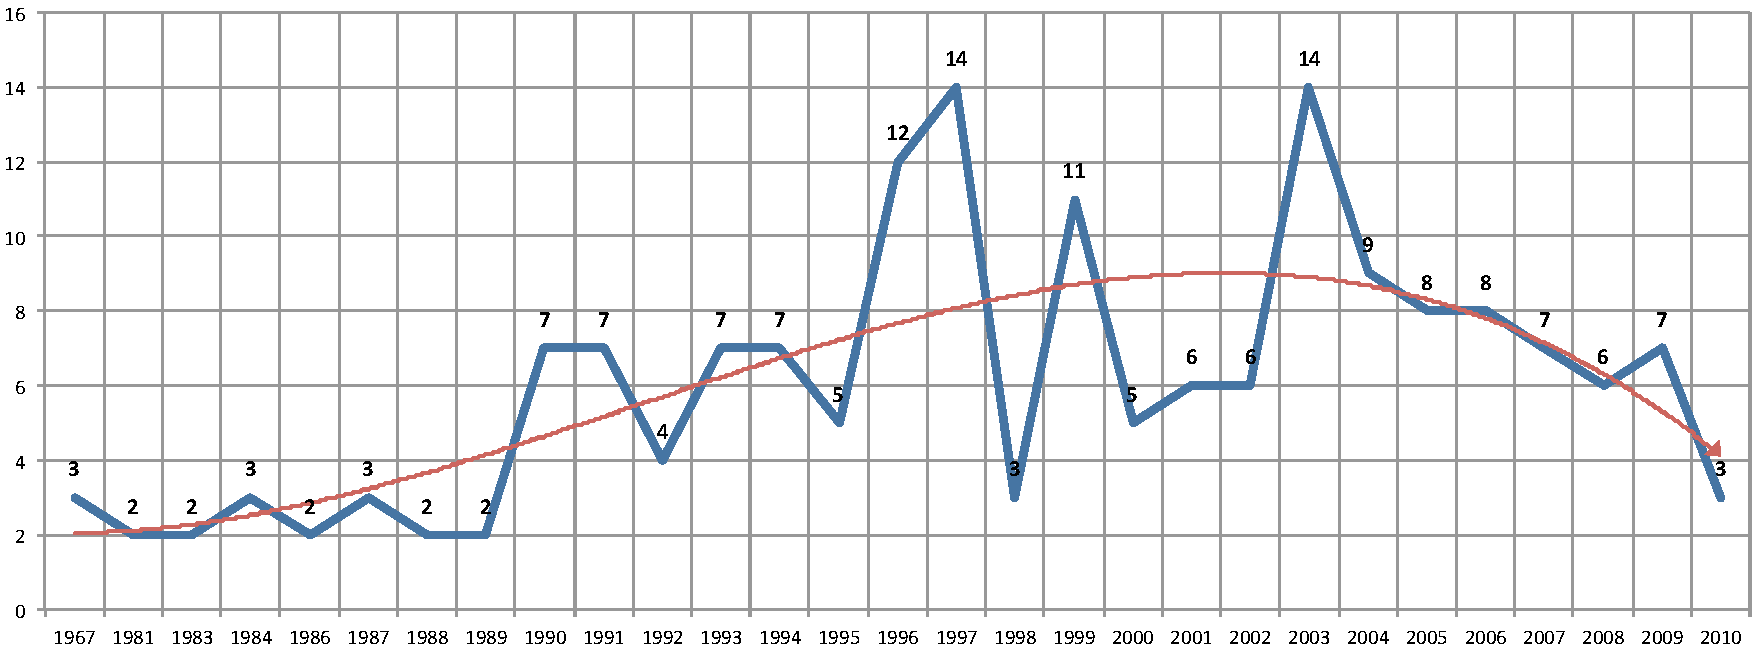
\includegraphics[scale=0.5]{abntex2-modelo-img-grafico.pdf}
	\end{center}
	\legend{Fonte: \citeonline[p. 24]{araujo2012}}
\end{figure}

% ---
\subsection{Figuras em \emph{minipages}}
% ---

\emph{Minipages} são usadas para inserir textos ou outros elementos em quadros
com tamanhos e posições controladas. Veja o exemplo da
\autoref{fig_minipage_imagem1} e da \autoref{fig_minipage_grafico2}.

\begin{figure}[htb]
 \label{teste}
 \centering
  \begin{minipage}{0.4\textwidth}
    \centering
    \caption{Imagem 1 da minipage} \label{fig_minipage_imagem1}
    
\includegraphics[scale=0.9]{abntex2-modelo-img-marca.pdf}
    \legend{Fonte: Produzido pelos autores}
  \end{minipage}
  \hfill
  \begin{minipage}{0.4\textwidth}
    \centering
    \caption{Grafico 2 da minipage} \label{fig_minipage_grafico2}
    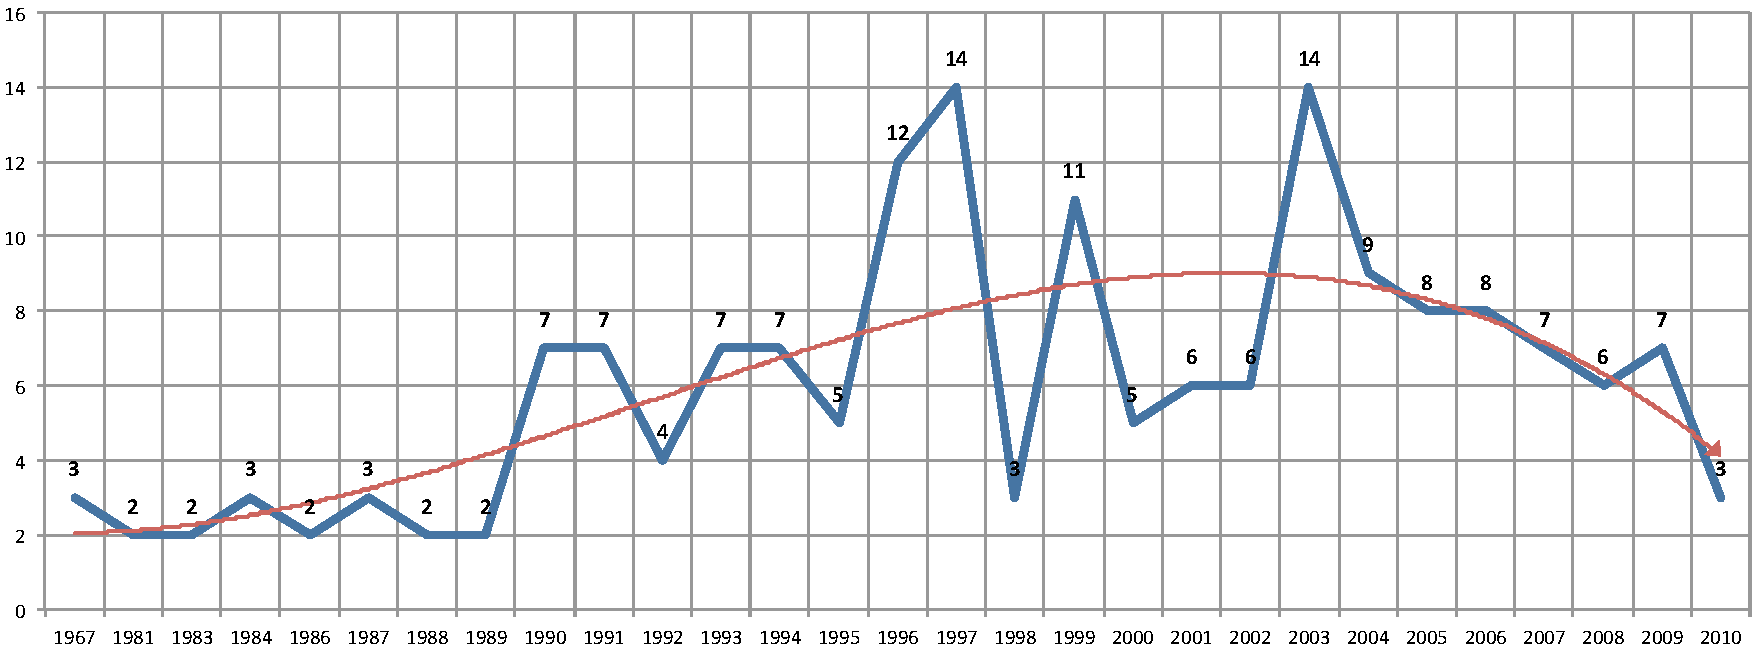
\includegraphics[scale=0.2]{abntex2-modelo-img-grafico.pdf}
    \legend{Fonte: \citeonline[p. 24]{araujo2012}}
  \end{minipage}
\end{figure}

Observe que, segundo a \citeonline[seções 4.2.1.10 e 5.8]{NBR14724:2011}, as
ilustrações devem sempre ter numeração contínua e única em todo o documento:

\begin{citacao}
Qualquer que seja o tipo de ilustração, sua identificação aparece na parte
superior, precedida da palavra designativa (desenho, esquema, fluxograma,
fotografia, gráfico, mapa, organograma, planta, quadro, retrato, figura,
imagem, entre outros), seguida de seu número de ordem de ocorrência no texto,
em algarismos arábicos, travessão e do respectivo título. Após a ilustração, na
parte inferior, indicar a fonte consultada (elemento obrigatório, mesmo que
seja produção do próprio autor), legenda, notas e outras informações
necessárias à sua compreensão (se houver). A ilustração deve ser citada no
texto e inserida o mais próximo possível do trecho a que se
refere. \cite[seções 5.8]{NBR14724:2011}
\end{citacao}

% ---
\section{Expressões matemáticas}
% ---

\index{expressões matemáticas}Use o ambiente \texttt{equation} para escrever
expressões matemáticas numeradas:

\begin{equation}
  \forall x \in X, \quad \exists \: y \leq \epsilon
\end{equation}

Escreva expressões matemáticas entre \$ e \$, como em $ \lim_{x \to \infty}
\exp(-x) = 0 $, para que fiquem na mesma linha.

Também é possível usar colchetes para indicar o início de uma expressão
matemática que não é numerada.

\[
\left|\sum_{i=1}^n a_ib_i\right|
\le
\left(\sum_{i=1}^n a_i^2\right)^{1/2}
\left(\sum_{i=1}^n b_i^2\right)^{1/2}
\]

Consulte mais informações sobre expressões matemáticas em
\url{https://github.com/abntex/abntex2/wiki/Referencias}.

% ---
\section{Enumerações: alíneas e subalíneas}
% ---

\index{alíneas}\index{subalíneas}\index{incisos}Quando for necessário enumerar
os diversos assuntos de uma seção que não possua título, esta deve ser
subdividida em alíneas \cite[4.2]{NBR6024:2012}:

\begin{alineas}

  \item os diversos assuntos que não possuam título próprio, dentro de uma mesma
  seção, devem ser subdivididos em alíneas; 
  
  \item o texto que antecede as alíneas termina em dois pontos;
  \item as alíneas devem ser indicadas alfabeticamente, em letra minúscula,
  seguida de parêntese. Utilizam-se letras dobradas, quando esgotadas as
  letras do alfabeto;

  \item as letras indicativas das alíneas devem apresentar recuo em relação à
  margem esquerda;

  \item o texto da alínea deve começar por letra minúscula e terminar em
  ponto-e-vírgula, exceto a última alínea que termina em ponto final;

  \item o texto da alínea deve terminar em dois pontos, se houver subalínea;

  \item a segunda e as seguintes linhas do texto da alínea começa sob a
  primeira letra do texto da própria alínea;
  
  \item subalíneas \cite[4.3]{NBR6024:2012} devem ser conforme as alíneas a
  seguir:

  \begin{alineas}
     \item as subalíneas devem começar por travessão seguido de espaço;

     \item as subalíneas devem apresentar recuo em relação à alínea;

     \item o texto da subalínea deve começar por letra minúscula e terminar em
     ponto-e-vírgula. A última subalínea deve terminar em ponto final, se não
     houver alínea subsequente;

     \item a segunda e as seguintes linhas do texto da subalínea começam sob a
     primeira letra do texto da própria subalínea.
  \end{alineas}
  
  \item no \abnTeX\ estão disponíveis os ambientes \texttt{incisos} e
  \texttt{subalineas}, que em suma são o mesmo que se criar outro nível de
  \texttt{alineas}, como nos exemplos à seguir:
  
  \begin{incisos}
    \item \textit{Um novo inciso em itálico};
  \end{incisos}
  
  \item Alínea em \textbf{negrito}:
  
  \begin{subalineas}
    \item \textit{Uma subalínea em itálico};
    \item \underline{\textit{Uma subalínea em itálico e sublinhado}}; 
  \end{subalineas}
  
  \item Última alínea com \emph{ênfase}.
  
\end{alineas}

% ---
\section{Espaçamento entre parágrafos e linhas}
% ---

\index{espaçamento!dos parágrafos}O tamanho do parágrafo, espaço entre a margem
e o início da frase do parágrafo, é definido por:

\begin{verbatim}
   \setlength{\parindent}{1.3cm}
\end{verbatim}

\index{espaçamento!do primeiro parágrafo}Por padrão, não há espaçamento no
primeiro parágrafo de cada início de divisão do documento
(\autoref{sec-divisoes}). Porém, você pode definir que o primeiro parágrafo
também seja indentado, como é o caso deste documento. Para isso, apenas inclua o
pacote \textsf{indentfirst} no preâmbulo do documento:

\begin{verbatim}
   \usepackage{indentfirst}      % Indenta o primeiro parágrafo de cada seção.
\end{verbatim}

\index{espaçamento!entre os parágrafos}O espaçamento entre um parágrafo e outro
pode ser controlado por meio do comando:

\begin{verbatim}
  \setlength{\parskip}{0.2cm}  % tente também \onelineskip
\end{verbatim}

\index{espaçamento!entre as linhas}O controle do espaçamento entre linhas é
definido por:

\begin{verbatim}
  \OnehalfSpacing       % espaçamento um e meio (padrão); 
  \DoubleSpacing        % espaçamento duplo
  \SingleSpacing        % espaçamento simples	
\end{verbatim}

Para isso, também estão disponíveis os ambientes:

\begin{verbatim}
  \begin{SingleSpace} ...\end{SingleSpace}
  \begin{Spacing}{hfactori} ... \end{Spacing}
  \begin{OnehalfSpace} ... \end{OnehalfSpace}
  \begin{OnehalfSpace*} ... \end{OnehalfSpace*}
  \begin{DoubleSpace} ... \end{DoubleSpace}
  \begin{DoubleSpace*} ... \end{DoubleSpace*} 
\end{verbatim}

Para mais informações, consulte \citeonline[p. 47-52 e 135]{memoir}.

% ---
\section{Inclusão de outros arquivos}\label{sec-include}
% ---

É uma boa prática dividir o seu documento em diversos arquivos, e não
apenas escrever tudo em um único. Esse recurso foi utilizado neste
documento. Para incluir diferentes arquivos em um arquivo principal,
de modo que cada arquivo incluído fique em uma página diferente, utilize o
comando:

\begin{verbatim}
   \include{documento-a-ser-incluido}      % sem a extensão .tex
\end{verbatim}

Para incluir documentos sem quebra de páginas, utilize:

\begin{verbatim}
   \input{documento-a-ser-incluido}      % sem a extensão .tex
\end{verbatim}

% ---
\section{Compilar o documento \LaTeX}
% ---

Geralmente os editores \LaTeX, como o
TeXlipse\footnote{\url{http://texlipse.sourceforge.net/}}, o
Texmaker\footnote{\url{http://www.xm1math.net/texmaker/}}, entre outros,
compilam os documentos automaticamente, de modo que você não precisa se
preocupar com isso.

No entanto, você pode compilar os documentos \LaTeX usando os seguintes
comandos, que devem ser digitados no \emph{Prompt de Comandos} do Windows ou no
\emph{Terminal} do Mac ou do Linux:

\begin{verbatim}
   pdflatex ARQUIVO_PRINCIPAL.tex
   bibtex ARQUIVO_PRINCIPAL.aux
   makeindex ARQUIVO_PRINCIPAL.idx 
   makeindex ARQUIVO_PRINCIPAL.nlo -s nomencl.ist -o ARQUIVO_PRINCIPAL.nls
   pdflatex ARQUIVO_PRINCIPAL.tex
   pdflatex ARQUIVO_PRINCIPAL.tex
\end{verbatim}

% ---
\section{Remissões internas}
% ---

Ao nomear a \autoref{tab-nivinv} e a \autoref{fig_circulo}, apresentamos um
exemplo de remissão interna, que também pode ser feita quando indicamos o
\autoref{cap_exemplos}, que tem o nome \emph{\nameref{cap_exemplos}}. O número
do capítulo indicado é \ref{cap_exemplos}, que se inicia à
\autopageref{cap_exemplos}\footnote{O número da página de uma remissão pode ser
obtida também assim:
\pageref{cap_exemplos}.}.
Veja a \autoref{sec-divisoes} para outros exemplos de remissões internas entre
seções, subseções e subsubseções.

O código usado para produzir o texto desta seção é:

\begin{verbatim}
Ao nomear a \autoref{tab-nivinv} e a \autoref{fig_circulo}, apresentamos um
exemplo de remissão interna, que também pode ser feita quando indicamos o
\autoref{cap_exemplos}, que tem o nome \emph{\nameref{cap_exemplos}}. O número
do capítulo indicado é \ref{cap_exemplos}, que se inicia à
\autopageref{cap_exemplos}\footnote{O número da página de uma remissão pode ser
obtida também assim:
\pageref{cap_exemplos}.}.
Veja a \autoref{sec-divisoes} para outros exemplos de remissões internas entre
seções, subseções e subsubseções.
\end{verbatim}

% ---
\section{Divisões do documento: seção}\label{sec-divisoes}
% ---

Esta seção testa o uso de divisões de documentos. Esta é a
\autoref{sec-divisoes}. Veja a \autoref{sec-divisoes-subsection}.

\subsection{Divisões do documento: subseção}\label{sec-divisoes-subsection}

Isto é uma subseção. Veja a \autoref{sec-divisoes-subsubsection}, que é uma
\texttt{subsubsection} do \LaTeX, mas é impressa chamada de ``subseção'' porque
no Português não temos a palavra ``subsubseção''.

\subsubsection{Divisões do documento: subsubseção}
\label{sec-divisoes-subsubsection}

Isto é uma subsubseção.

\subsubsection{Divisões do documento: subsubseção}

Isto é outra subsubseção.

\subsection{Divisões do documento: subseção}\label{sec-exemplo-subsec}

Isto é uma subseção.

\subsubsection{Divisões do documento: subsubseção}

Isto é mais uma subsubseção da \autoref{sec-exemplo-subsec}.


\subsubsubsection{Esta é uma subseção de quinto
nível}\label{sec-exemplo-subsubsubsection}

Esta é uma seção de quinto nível. Ela é produzida com o seguinte comando:

\begin{verbatim}
\subsubsubsection{Esta é uma subseção de quinto
nível}\label{sec-exemplo-subsubsubsection}
\end{verbatim}

\subsubsubsection{Esta é outra subseção de quinto nível}\label{sec-exemplo-subsubsubsection-outro}

Esta é outra seção de quinto nível.


\paragraph{Este é um parágrafo numerado}\label{sec-exemplo-paragrafo}

Este é um exemplo de parágrafo nomeado. Ele é produzida com o comando de
parágrafo:

\begin{verbatim}
\paragraph{Este é um parágrafo nomeado}\label{sec-exemplo-paragrafo}
\end{verbatim}

A numeração entre parágrafos numeradaos e subsubsubseções são contínuas.

\paragraph{Esta é outro parágrafo numerado}\label{sec-exemplo-paragrafo-outro}

Esta é outro parágrafo nomeado.

% ---
\section{Este é um exemplo de nome de seção longo. Ele deve estar
alinhado à esquerda e a segunda e demais linhas devem iniciar logo abaixo da
primeira palavra da primeira linha}
% ---

Isso atende à norma \citeonline[seções de 5.2.2 a 5.2.4]{NBR14724:2011} 
 e \citeonline[seções de 3.1 a 3.8]{NBR6024:2012}.

% ---
\section{Diferentes idiomas e hifenizações}
\label{sec-hifenizacao}
% ---

Para usar hifenizações de diferentes idiomas, inclua nas opções do documento o
nome dos idiomas que o seu texto contém. Por exemplo (para melhor
visualização, as opções foram quebras em diferentes linhas):

\begin{verbatim}
\documentclass[
	12pt,
	openright,
	twoside,
	a4paper,
	english,
	french,
	spanish,
	brazil
	]{abntex2}
\end{verbatim}

O idioma português-brasileiro (\texttt{brazil}) é incluído automaticamente pela
classe \textsf{abntex2}. Porém, mesmo assim a opção \texttt{brazil} deve ser
informada como a última opção da classe para que todos os pacotes reconheçam o
idioma. Vale ressaltar que a última opção de idioma é a utilizada por padrão no
documento. Desse modo, caso deseje escrever um texto em inglês que tenha
citações em português e em francês, você deveria usar o preâmbulo como abaixo:

\begin{verbatim}
\documentclass[
	12pt,
	openright,
	twoside,
	a4paper,
	french,
	brazil,
	english
	]{abntex2}
\end{verbatim}

A lista completa de idiomas suportados, bem como outras opções de hifenização,
estão disponíveis em \citeonline[p.~5-6]{babel}.

Exemplo de hifenização em inglês\footnote{Extraído de:
\url{http://en.wikibooks.org/wiki/LaTeX/Internationalization}}:

\begin{otherlanguage*}{english}
\textit{Text in English language. This environment switches all language-related
definitions, like the language specific names for figures, tables etc. to the other
language. The starred version of this environment typesets the main text
according to the rules of the other language, but keeps the language specific
string for ancillary things like figures, in the main language of the document.
The environment hyphenrules switches only the hyphenation patterns used; it can
also be used to disallow hyphenation by using the language name
`nohyphenation'.}
\end{otherlanguage*}

Exemplo de hifenização em francês\footnote{Extraído de:
\url{http://bigbrowser.blog.lemonde.fr/2013/02/17/tu-ne-tweeteras-point-le-vatican-interdit-aux-cardinaux-de-tweeter-pendant-le-conclave/}}:

\begin{otherlanguage*}{french}
\textit{Texte en français. Pas question que Twitter ne vienne faire une
concurrence déloyale à la traditionnelle fumée blanche qui marque l'élection
d'un nouveau pape. Pour éviter toute fuite précoce, le Vatican a donc pris un
peu d'avance, et a déjà interdit aux cardinaux qui prendront part au vote
d'utiliser le réseau social, selon Catholic News Service. Une mesure valable
surtout pour les neuf cardinaux – sur les 117 du conclave – pratiquants très
actifs de Twitter, qui auront interdiction pendant toute la période de se
connecter à leur compte.}
\end{otherlanguage*}

Pequeno texto em espanhol\footnote{Extraído de:
\url{http://internacional.elpais.com/internacional/2013/02/17/actualidad/1361102009_913423.html}}:

\foreignlanguage{spanish}{\textit{Decenas de miles de personas ovacionan al pontífice en su
penúltimo ángelus dominical, el primero desde que anunciase su renuncia. El Papa se
centra en la crítica al materialismo}}.

O idioma geral do texto por ser alterado como no exemplo seguinte:

\begin{verbatim}
  \selectlanguage{english}
\end{verbatim}

Isso altera automaticamente a hifenização e todos os nomes constantes de
referências do documento para o idioma inglês. Consulte o manual da classe
\cite{abntex2classe} para obter orientações adicionais sobre internacionalização de
documentos produzidos com \abnTeX.

A \autoref{sec-citacao} descreve o ambiente \texttt{citacao} que pode receber
como parâmetro um idioma a ser usado na citação.

% ---
\section{Consulte o manual da classe \textsf{abntex2}}
% ---

Consulte o manual da classe \textsf{abntex2} \cite{abntex2classe} para uma
referência completa das macros e ambientes disponíveis. 

Além disso, o manual possui informações adicionais sobre as normas ABNT
observadas pelo \abnTeX\ e considerações sobre eventuais requisitos específicos
não atendidos, como o caso da \citeonline[seção 5.2.2]{NBR14724:2011}, que
especifica o espaçamento entre os capítulos e o início do texto, regra
propositalmente não atendida pelo presente modelo.

% ---
\section{Referências bibliográficas}
% ---

A formatação das referências bibliográficas conforme as regras da ABNT são um
dos principais objetivos do \abnTeX. Consulte os manuais
\citeonline{abntex2cite} e \citeonline{abntex2cite-alf} para obter informações
sobre como utilizar as referências bibliográficas.

%-
\subsection{Acentuação de referências bibliográficas}
%-

Normalmente não há problemas em usar caracteres acentuados em arquivos
bibliográficos (\texttt{*.bib}). Porém, como as regras da ABNT fazem uso quase
abusivo da conversão para letras maiúsculas, é preciso observar o modo como se
escreve os nomes dos autores. Na ~\autoref{tabela-acentos} você encontra alguns
exemplos das conversões mais importantes. Preste atenção especial para `ç' e `í'
que devem estar envoltos em chaves. A regra geral é sempre usar a acentuação
neste modo quando houver conversão para letras maiúsculas.

\begin{table}[htbp]
\caption{Tabela de conversão de acentuação.}
\label{tabela-acentos}

\begin{center}
\begin{tabular}{ll}\hline\hline
acento & \textsf{bibtex}\\
à á ã & \verb+\`a+ \verb+\'a+ \verb+\~a+\\
í & \verb+{\'\i}+\\
ç & \verb+{\c c}+\\
\hline\hline
\end{tabular}
\end{center}
\end{table}


% ---
\section{Precisa de ajuda?}
% ---

Consulte a FAQ com perguntas frequentes e comuns no portal do \abnTeX:
\url{https://github.com/abntex/abntex2/wiki/FAQ}.

Inscreva-se no grupo de usuários \LaTeX:
\url{http://groups.google.com/group/latex-br}, tire suas dúvidas e ajude
outros usuários.

Participe também do grupo de desenvolvedores do \abnTeX:
\url{http://groups.google.com/group/abntex2} e faça sua contribuição à
ferramenta.

% ---
\section{Você pode ajudar?}
% ---

Sua contribuição é muito importante! Você pode ajudar na divulgação, no
desenvolvimento e de várias outras formas. Veja como contribuir com o \abnTeX\
em \url{https://github.com/abntex/abntex2/wiki/Como-Contribuir}.

% ---
\section{Quer customizar os modelos do \abnTeX\ para sua instituição ou
universidade?}
% ---

Veja como customizar o \abnTeX\ em:
\url{https://github.com/abntex/abntex2/wiki/ComoCustomizar}.


% ---

%\chapter{Conteúdos específicos do modelo de trabalho acadêmico}\label{cap_trabalho_academico}

%\section{Quadros}

%Este modelo vem com o ambiente \texttt{quadro} e impressão de Lista de quadros 
%configurados por padrão. Verifique um exemplo de utilização:

%\begin{quadro}[htb]
%\caption{\label{quadro_exemplo}Exemplo de quadro}
%\begin{tabular}{|c|c|c|c|}
%	\hline
%	\textbf{Pessoa} & \textbf{Idade} & \textbf{Peso} & \textbf{Altura} \\ \hline
%	Marcos & 26    & 68   & 178    \\ \hline
%	Ivone  & 22    & 57   & 162    \\ \hline
%	...    & ...   & ...  & ...    \\ \hline
%	Sueli  & 40    & 65   & 153    \\ \hline
%\end{tabular}
%\fonte{Autor.}
%\end{quadro}

%Este parágrafo apresenta como referenciar o quadro no texto, requisito
%obrigatório da ABNT. 
%Primeira opção, utilizando \texttt{autoref}: Ver o \autoref{quadro_exemplo}. 
%Segunda opção, utilizando  \texttt{ref}: Ver o Quadro \ref{quadro_exemplo}.

% ----------------------------------------------------------
% PARTE
% ----------------------------------------------------------
%\part{Referenciais teóricos}
% ----------------------------------------------------------

% ---
% Capitulo de revisão de literatura
% ---
\chapter{Revisão de Literatura}
% ---
Neste tópico é revisado o histórico do uso da tecnologia na gestão de negócios de hotelaria na literatura científica, com o objetivo de contextualizar e destacar a relevância do projeto.

\subsection{Histórico do Turismo e da Hospitalidade} 
A atividade de turismo é o ato de uma pessoa de se deslocar para um local diverso da sua residência por diferentes motivações, desde econômicas, que datam a antiguidade com as grandes viagens exploratórias dos povos antigos, até em entretenimento.  A partir do século XVII, os avanços tecnológicos em diferentes setores mudaram profundamente o modo de vida do homem e suas relações sociais, o que fortaleceu o turismo de entretenimento, que se tornou um forte pilar econômico para diferentes regiões do mundo~\cite{ignarra2013}.

No Brasil em 2024, segundo a Federação do Comércio de Bens, Serviços e Turismo do Estado de São Paulo~\cite{fecomercio2024}, o setor do turismo cresceu 4,3\% em relação a 2023, o que gerou um faturamento de 207 bilhões de reais. Sendo que, o estado de São Paulo representou 34\% do rendimento total. Fato que expõe a importância do turismo para a economia  do país, além da força das regiões turísticas do estado de São Paulo. 

Historicamente, como consequência do crescimento do turismo, houve o aumento de estruturas físicas e sociais para atender as necessidades dos viajantes, dentre elas, os meios de hospedagem. Dentro do serviço de hospedagem existem diferentes tipos de estrutura, entre elas a pousada. Segundo \citeonline{zanella2006}, a pousada é um ambiente pequeno e de arquitetura simples que presta serviços de hospedagem, alimentação e lazer, de forma criativa e personalizada. 

\subsection{A Gestão Hoteleira e o Impacto da Tecnologia}
Uma pousada, como outros negócios, precisa promover um processo de gestão de seus serviços com o objetivo de atender as expectativas dos clientes, melhorar a satisfação e retê-los~\cite{zanella2006}. A gestão de um empreendimento de hospedagem é geralmente departamentalizada em: Hospedagem, Marketing, Finanças e Contabilidade, Administração e Segurança, Alimentos e Bebidas; e Eventos e Serviços Diversos. Essa estrutura varia de acordo com a categoria da hotelaria, mas que é fundamental para a coordenação das atividades, atração de hóspedes e geração de lucro~\cite{martins2011}.

De acordo com \citeonline{sidonio2015}, com o aumento da concorrência e as mudanças nos hábitos dos clientes decorrentes da globalização, para atingir seus objetivos, uma empresa hoteleira deve sempre buscar informações para o embasamento das tomadas de decisões tanto de planejamento quanto de inovação dos seus serviços. Dessa forma,  a gestão hoteleira exige que o gestor esteja atento às constantes mudanças nas tendências do mercado contemporâneo, devendo ser ágil e prático nas suas tomadas de decisão~\cite{mauricio2011}. Nesse contexto, as tecnologias da informação surgem nesse setor como ferramentas capazes de auxiliar no aumento da competitividade da empresa hoteleira~\cite{buhalis1998}. 

A tecnologia afeta a competitividade das empresas através do fornecimento de benefícios estratégicos. Isso porque, essa ajuda o acesso a informações que auxiliam as empresas na customização dos seus produtos e serviços,  na garantia de preços competitivos, diminuição dos custos associado a um aumento de eficiência e na construção de relacionamentos mais próximos com fornecedores e clientes. Assim, o setor do turismo, sendo uma área que precisa estar sempre se adaptando às necessidades do mercado e do cliente, é altamente beneficiado pelo uso das novas tecnologias~\cite{buhalis1998}.

Dessa forma, o uso de sistema computacionais, conjunto de componentes que permitem a entrada, processamento e saída de dados é bastante útil no que tange a gestão de empresas hospitaleiras. Visto que, otimiza e facilita o acesso a dados que constituem informações precisas,  que são importantes para o sucesso do negócio~\cite{zeferino2012}.
% ----------------------------------------------------------
% TÓPICO: GESTÃO DO PROJETO
\chapter{Gestão do Projeto}
Esta seção detalha as principais estratégias de gestão aplicadas no desenvolvimento da aplicação web de gestão para a pousada Chalés Água de Coco. Dessa forma, nela são apresentadas as metodologias, ferramentas e práticas que foram adotadas para o planejamento, execução e monitoramento do projeto, com o objetivo de garantir uma entrega organizada, eficiente e alinhada aos objetivos estabelecidos pelas partes interessadas.
% 
\section{Organização da Equipe}
  Na gestão desse projeto, a organização da equipe representou um marco fundamental e teve como foco dividir as funções e atividades necessárias para o desenvolvimento da aplicação web de gestão da pousada entre os membros.%
\subsection{Funções e Responsabilidades}
A divisão das funções e responsabilidades foi realizada de maneira estratégica e levou em consideração as competências técnicas de cada membro da equipe, visando a entrega do produto final dentro do prazo e escopo estipulados. 	A função de cada membro e suas respectivas responsabilidades estão detalhadas no \autoref{quadro_funcao_responsabilidade}.
%	
\FloatBarrier
\begin{quadro}[H]
	\caption{Divisão das Funções e Responsabilidades da Equipe do Projeto}
	\label{quadro_funcao_responsabilidade}
	\renewcommand{\arraystretch}{1.3} % Aumenta o espaçamento entre linhas
	\begin{tabular}{|>{\raggedright\arraybackslash}m{3cm} 
			|>{\raggedright\arraybackslash}m{4.5cm} 
			|>{\raggedright\arraybackslash}m{6.7cm}|}
		\hline
		\textbf{Integrante} & \textbf{Função} & \textbf{Responsabilidades} \\ \hline
		Anna Julia & Analista de Cronograma & Criar, manter e monitorar o cronograma do projeto, além de oferecer suporte às práticas de gestão. \\ \hline
		Guilherme Akio & Engenheiro de Dados (DBA) & Implementar, administrar e otimizar o banco de dados da aplicação, garantindo integridade, segurança e performance dos dados. \\ \hline
		Guilherme Bittencourt & Documentador Técnico e Engenheiro de \textit{Software} & Criar e manter a documentação técnica com clareza e acessibilidade. Definir e organizar a estrutura da aplicação. \\ \hline
		Kelly Radchelle & Gerente de Projeto & Coordenar a equipe e gerenciar as atividades do projeto, facilitando a tomada de decisões e assegurando a comunicação entre as partes interessadas. \\ \hline
		Rafael Teixeira & Desenvolvedor \textit{Frontend} & Criar e implementar a interface da aplicação, garantindo boa experiência do usuário (UX) e design de interface (UI), além de desenvolver a lógica de apresentação. \\ \hline
		Ricardo Carriel & Desenvolvedor \textit{Backend} & Desenvolver a lógica de negócio, configurar e administrar o servidor, garantindo a integração e funcionamento da aplicação. \\ \hline
	\end{tabular}
	\fonte{Elaborado pelos autores.}
\end{quadro}
%
\section{Metodologias de Gestão e Desenvolvimento}
Para assegurar que a entrega do produto final ocorresse dentro do prazo estipulado e estivesse em pleno alinhamento com as expectativas da cliente, a equipe envolvida no projeto optou pela adoção da metodologia ágil \textit{Scrum} como ferramenta de gestão e desenvolvimento do projeto. Essa decisão fundamentou-se na familiaridade da equipe com a estrutura, na capacidade do \textit{Scrum} de otimizar a organização, divisão e planejamento de atividades do projeto, e em sua relevância como framework de gerenciamento– dado seu uso extensivo no contexto de desenvolvimento de softwares complexos.

Segundo Schwaber e Sutherland \cite{scrumguide}, o \textit{Scrum} é um \textit{framework} estruturado desenvolvido na década de 1990, com o objetivo de auxiliar equipes na criação e gerenciamento de produtos complexos. Por isso,  o \textit{Scrum} tem como pilares fundamentais a transparência, a inspeção e a adaptação. A transparência garante que todos os aspectos significativos do processo estejam visíveis e claros para as partes interessadas a todo momento. Enquanto a inspeção envolve o acompanhamento regular dos artefatos e progresso, auxiliando na identificação precoce de problemas e garantindo a transparência dos processos. Seguida pela adaptação que refere-se à capacidade de fazer ajustes no processo  em resposta aos problemas anteriormente identificados na inspeção, com o objetivo de otimizar os resultados da equipe.

Sabendo que para operacionalizar esses pilares e assegurar um ciclo de desenvolvimento iterativo e incremental, a metodologia \textit{Scrum} sugere a definição de papeis específicos dentro do time, estabelece a realização de uma sequência de eventos formais e o uso de artefatos específicos, os integrantes da equipe desenvolveram as tarefas e eventos sugeridos pelo \textit{Scrum} para a gestão e desenvolvimento do projeto.
%
\subsection{Time Scrum}
Como estabelecido no Guia do Scrum \cite{scrumguide}, os membros da equipe do projeto assumem papeis específicos que compõem um \textit{time Scrum}: \textit{Product Owner}, \textit{Scrum Master} e Time de Desenvolvimento. 
%
\begin{enumerate}[label=\roman*)]
	\item O \textit{Product Owner} é o representante das partes interessadas (\textit{Stakeholders}) e tem como responsabilidade principal gerenciar o \textit{backlog} do produto. Seu objetivo é maximizar o valor do produto para o usuário final e otimizar o trabalho do Time de Desenvolvimento. 
	\item O \textit{Scrum Master}  é o responsável por promover e facilitar a aplicação da teoria e das práticas do \textit{framework}, a fim de ajudar a equipe a superar problemas que possam afetar seu progresso. 
	\item O Time de Desenvolvimento é responsável por entregar um incremento (versão potencialmente usável do produto) ao final de cada \textit{sprint}, atuando de maneira auto-organizada e multifuncional.
\end{enumerate}
%

Diante disso, houve a distribuição dos papeis de um \textit{time Scrum} entre os integrantes da equipe registrada na \autoref{quadro:time_scrum}.
%
\begin{quadro}[H]
	\centering
	\caption{Função dos Integrantes da Equipe}
	\label{quadro:time_scrum}
	\begin{tabular}{|>{\centering\arraybackslash}m{3.2cm}|>{\centering\arraybackslash}m{3.5cm}|>{\centering\arraybackslash}m{3.5cm}|>{\centering\arraybackslash}m{4cm}|}
		\hline
		\multirow{2}{*}{\textbf{Integrante}} & \multicolumn{3}{c|}{\textbf{Função}} \\ \cline{2-4}
		&\textit{Product Owner} & \textit{Scrum Master} & Time de Desenvolvimento \\ \hline 
		Anna Julia &  & X & \\ \hline Guilherme Akio & & & X \\ \hline Guilherme Bittencourt & & & X \\ \hline Kelly Radchelle & X & & \\ \hline Rafael Teixeira & & & X \\ \hline Ricardo Carriel & & & X \\ \hline
	\end{tabular}
	\fonte{Elaborado pelos autores.}
\end{quadro}
%---

%---
\section{Artefatos}
No Scrum,  os artefatos são elementos que ajudam a equipe a consolidar a transparência no processo de desenvolvimento. Cientes das suas importâncias, o \textit {time scrum} realizou o planejamento inicial dos artefatos:  \textit {Product Backlog} e \textit {Sprints Backlog}.
%
\subsection{Product Backlog}
No Guia do Scrum \cite{scrumguide}, o \textit{product Backlog} é definido como uma lista ordenada de todos os itens de trabalho, incluindo funcionalidades e requisitos necessários para a produção do produto, que oferecem o máximo valor e utilidade para o cliente.

Ciente disso, o \textit{product owner} do projeto elaborou o \textit{product backlog} inicial da aplicação \textit{web} de gestão da pousada Chalés Água de Coco (\autoref{product_backlog}), com base nas histórias de usuário levantadas pela equipe. Isso porque, elas refletem fielmente as necessidades e expectativas da usuária e principal \textit {stakeholder} garantindo que o desenvolvimento em total alinhamento.
%
\begin{quadro}[H]
	\caption{Product Backlog - Parte 1}
	\label{product_backlog}
	\begin{tabular}{|>{\centering\arraybackslash}m{1.4cm}|>{\raggedright\arraybackslash}m{6.5cm}|>{\raggedright\arraybackslash}m{3.8cm}|>{\raggedright\arraybackslash}m{2.5cm}|}
		\hline
		\textbf{Código} & \textbf{Item} & \textbf{Categoria} & \textbf{Prioridade} \\ \hline
		1 & Definir e configurar ambiente de desenvolvimento & Requisito Técnico   & ALTA    \\ \hline
		2 & Definir ambiente de hospedagem/publicação & Requisito Técnico & ALTA  \\ \hline
		3 & Organizar repositório e fluxo Git  & Requisito Técnico & ALTA\\ \hline
		4 & Levantar requisitos funcionais e não funcionais    & Modelagem de dados & ALTA    \\ \hline
		5 & Mapear casos de uso & Modelagem de dados   & ALTA  \\ \hline
		6 & Documentar o levantamento e registrar os requisitos    & Documentação   & ALTA    \\ \hline
		7 & Criar Modelo Entidade-Relacionamento (MER)    & Modelagem de dados   & ALTA    \\ \hline
		8 & Criar Diagrama de Entidade-Relacionamento (DER)    & Modelagem de dados   & ALTA    \\ \hline
		9 & Criar Diagrama de Componentes    & Arquitetura   & ALTA    \\ \hline
		10 & Criar Diagrama de Implantação    & Arquitetura   & ALTA    \\ \hline
		11 & Documentar os diagramas produzidos & Documentação &
		ALTA \\ \hline
		12 & Configurar ambiente do servidor & Requisito Técnico &
		ALTA \\ \hline
		13 & Configurar banco de dados PostgreSQL & Requisito Técnico &
		ALTA \\ \hline
		14 & Implementar login e logout de usuário & Autenticação e Segurança & ALTA \\ \hline
		15 & Criar funcionalidade de cadastro de quartos & Gestão de Quartos & ALTA \\ \hline
		16 & Criar funcionalidade de exclusão de cadastro de quartos &
		Gestão de Quartos & MÉDIA \\ \hline
		17 & Criar funcionalidade de listagem de quartos & Gestão de Quartos & MÉDIA \\ \hline
		18 & Criar funcionalidade de edição do cadastro de quartos &
		Gestão de Quartos &	MÉDIA \\ \hline
	\end{tabular}
		\fonte{Elaborado pelos autores.}
\end{quadro}
%
\begin{quadro}[H]
	\caption{Product Backlog - Parte 2}
	\label{product_backlog_2}
	\begin{tabular}{|c|p{6.5cm}|p{3.8cm}|c|}
		\hline
		\textbf{Código} & \textbf{Item} & \textbf{Categoria} & \textbf{Prioridade} \\	\hline	
		19 & Criar interfaces para gestão de quartos & Gestão de Quartos & MÉDIA \\ \hline
		20 & Implementar funcionalidade de alteração manual do status (disponível, indisponível, em manutenção) do quarto & Gestão de Quartos & MÉDIA \\ \hline
		21 & Criar funcionalidade de cadastro de hóspedes &	Gestão de Hóspedes & ALTA \\ \hline
		22 & Criar funcionalidade de exclusão do cadastro de hóspedes &
		Gestão de Hóspedes & MÉDIA \\
		23 & Criar funcionalidade de edição do cadastro de hóspedes &
		Gestão de Hóspedes & MÉDIA \\ \hline
		24 & Criar interfaces para gestão de hóspedes &	Gestão de Hóspedes & MÉDIA \\ \hline
		25 & Criar funcionalidade de cadastro de reservas &	Gestão de Reservas & ALTA \\ \hline
		26 & Criar funcionalidade de exclusão do cadastro de reservas &
		Gestão de Reservas & ALTA \\ \hline
		27 & Criar funcionalidade de edição do cadastro de reservas &
		Gestão de Reservas & ALTA \\ \hline
		28 & Criar interfaces para gestão de Reservas &	Gestão de Reservas & ALTA \\ \hline
		29 & Criar funcionalidade para visualização do histórico de reservas por hóspede & Gestão de Reservas &	MÉDIA \\ \hline
		30 & Criar lógica de validação de disponibilidade de quartos para reservas & Gestão de Reservas & ALTA \\ \hline
		31 & Implementar atualização automática do status do quarto para “ocupado” após o \textit {check-in} & \textit {Check-in} e \textit {Check-out} & ALTA 
		\\ \hline
		32 & Criar funcionalidade de atualização do \textit {check-out} &
		\textit {Check-in} e \textit {Check-out} &	ALTA \\ \hline
		33 & Integrar ambientes, \textit{back-end} e \textit {front-end} &	Requisito técnico & ALTA \\ \hline
		34 & Documentar a configuração e o código desenvolvido &
		Documentação & ALTA \\ \hline
		35 & Criar funcionalidade de cadastro de receitas &	Gestão Financeira & BAIXA \\ \hline
	\end{tabular}
     \fonte{Elaborado pelos autores.}
     \end{quadro}
 % 
 \begin{quadro}[H]
     \caption{Product Backlog - Parte 3}
     	\label{product_backlog_3}
     	\begin{tabular}{|>{\centering\arraybackslash}m{1.4cm}|>{\raggedright\arraybackslash}m{6.5cm}|>{\raggedright\arraybackslash}m{3.8cm}|>{\raggedright\arraybackslash}m{2.5cm}|}
     		\hline
     		\textbf{Código} & \textbf{Item} & \textbf{Categoria} & \textbf{Prioridade} \\	\hline
     		36 & Criar funcionalidade para registrar comprovação de pagamento de reservas &	Gestão Financeira/Gestão de Reservas &
     		BAIXA \\ \hline
     		37 & Criar funcionalidade de exclusão do cadastro de receitas &
     		Gestão Financeira &	BAIXA \\ \hline
     		38 & Criar funcionalidade de edição do cadastro de receitas &
     		Gestão Financeira &	BAIXA \\ \hline
     		39 & Criar interface para gestão de receitas & Gestão Financeira & BAIXA \\ \hline
     		40 & Criar funcionalidade de cadastro de despesas &
     		Gestão Financeira & BAIXA \\ \hline
     		41 & Criar funcionalidade de exclusão do cadastro de despesas &
     		Gestão Financeira &	BAIXA \\ \hline
     		42 & Criar funcionalidade de edição do cadastro de despesas &
     		Gestão Financeira &	BAIXA \\ \hline   
     		43 & Criar interface para gestão de despesas & Gestão Financeira & BAIXA \\ \hline
     		44 & Criar funcionalidade para criar relatórios de quartos &
     		Gestão Financeira &	BAIXA \\ \hline
    		45 & Criar funcionalidade para criar relatórios de hóspedes &
    		Gestão Financeira &	BAIXA \\ \hline
     		46 & Criar funcionalidade para criar relatórios de reservas &
     		Gestão Financeira &	BAIXA \\ \hline
     		47 & Criar balanço financeiro simples (receitas, despesas, saldo) por período & Gestão Financeira & BAIXA \\ \hline
     		48 & Criar funcionalidade de filtragem de receita/despesa (data, categoria) &	Gestão Financeira & BAIXA \\ \hline
     		49 & implementar envio de notificação (\textit {e-mail}) para hóspede após confirmação da reserva & Notificações &
     		BAIXA \\ \hline
     		50 & Implementar criptografia &	Autenticação e Segurança &
     		BAIXA \\ \hline
     		51 & Definir escopo dos testes & Testes & MÉDIA \\ \hline
     		52 & Identificar cenários de teste & Testes & MÉDIA \\ \hline
     		53 & Elaborar casos de teste & Testes & MÉDIA \\ \hline
	     	54 & Definir as ferramentas de teste & Testes &	MÉDIA \\ \hline
	     	55 & Estabelecer ambiente de teste & Testes & MÉDIA \\ \hline
     	\end{tabular}
     		\fonte{Elaborado pelos autores.}
     		\end{quadro}

 \begin{quadro}[H]
	\caption{Product Backlog - Parte 4}
	\label{product_backlog_4}
	\begin{tabular}{|>{\centering\arraybackslash}m{1.4cm}|>{\raggedright\arraybackslash}m{6.5cm}|>{\raggedright\arraybackslash}m{3.8cm}|>{\raggedright\arraybackslash}m{2.5cm}|}
		\hline
		\textbf{Código} & \textbf{Item} & \textbf{Categoria} & \textbf{Prioridade} \\	\hline
			56 & Definir critérios de aceitação & Testes & MÉDIA \\ \hline
			57 & Preparar dados de teste & Testes &	MÉDIA \\ \hline
			58 & Executar testes gerais & Testes & MÉDIA \\ \hline
			59 & Executar testes SSL & Testes &	MÉDIA \\ \hline
			60 & Analisar e otimizar \textit {headers} de segurança &
			Autenticação e Segurança &	MÉDIA \\ \hline	
			61 & Realizar ajustes de segurança & Autenticação e Segurança
			& MÉDIA \\ \hline
			62 & Documentar resultados dos testes &	Testes & MÉDIA \\ \hline
			63 & Documentar componentes e estilos & Documentação &
			ALTA \\ \hline
			64 & Documentar o plano e a execução de testes & Documentação &
			MÉDIA \\ \hline
			65 & Registrar escolhas e mudanças de rumo & Documentação &
			ALTA \\ \hline
			66 & Documentar problemas ocorridos e lições aprendidas &
			Documentação & ALTA \\ \hline
			67 & Elaborar o plano de implantação & Implantação & 
			MÉDIA \\ \hline
			68 & Realizar implantação do sistema & Implantação & MÉDIA \\ \hline
			69 & Revisão final da documentação técnica & Documentação &
			ALTA \\ \hline
			70 & Treinamento da proprietária da pousada para uso da aplicação &	Implantação & MÉDIA \\ \hline
   \end{tabular}
   \fonte{Elaborado pelos autores.}
\end{quadro}
% ---
\subsection{Sprint Backlog}
O \textit{Sprint Backlog} é um plano elaborado pelo time de desenvolvimento, formado por um conjunto de itens selecionados da \textit {product backlog}. Esse plano possui um período de tempo determinado para sua realização, chamado de \textit {sprint}. 

Esse artefato promove a transparência das atividades do projeto, tornando visíveis e acessíveis para todos os membros da equipe as atividades que devem ser realizadas na \textit {Sprint}, garantindo que todos estejam cientes do que está sendo desenvolvido. Por isso, o time implementou o \autoref{sprints_backlog} que registra todas as \textit {Sprints Backlog} planejadas para o decorrer do projeto.

Para isso, considerando a flexibilidade oferecida por essa metodologia dividiu-se as \textit {sprints} do projeto em períodos de quinze dias (duas semanas), período dentro do estipulado pelo Guia do Scrum \cite{scrumguide}. Essa escolha de duração para as \textit {Sprints} levou em consideração que a equipe atuaria majoritariamente de forma remota, com tempo diário individual limitado para o trabalho. Este contexto demandava prazos mais longos para a execução das tarefas.

As atividades incluídas nas \textit{sprints backlog} foram baseadas nos itens da \textit{product Backlog}, no prazo de entrega do MVP e nas demais tarefas essenciais do projeto, como realização de testes e a elaboração da documentação técnica.
\\
\begin{quadro}[H]
	\caption{Sprints Backlog - Parte 1} 
	\label{sprints_backlog_1} 
	\begin{tabular}{|>{\centering\arraybackslash}m{1.5cm}|>{\raggedright\arraybackslash}m{2.5cm}|>{\raggedright\arraybackslash}m{3.2cm}|>{\raggedright\arraybackslash}m{7cm}|}
	\hline
	\textbf{Sprint} & \textbf{Período} & \textbf{Objetivo} & \textbf{Atividades} \\
		\hline
		1 & 08/04/2025 a 22/04/2025 & Realizar o planejamento do projeto  &
		- Definir e configurar ambiente de desenvolvimento. \newline
		- Definir ambiente de hospedagem/publicação. \newline
		- Organizar repositório e fluxo Git. \\
		\hline
		2 & 22/04/2025 a 06/05/2025 & Iniciar a fase de modelagem e documentação dos requisitos &
		- Levantar requisitos funcionais e não funcionais. \newline
		- Mapear casos de uso. \newline
		- Documentar o levantamento e registrar os requisitos. \\
		\hline
		3 & 06/05/2025 a 20/05/2025 & Finalizar a modelagem de dados e definir a arquitetura do sistema &
		- Criar do Diagrama de Componentes. \newline
		- Criar do Diagrama de Implantação. \newline
		- Criar do modelo relacional (MER). \newline
		- Criar do Diagrama de Entidade e Relacionamento (DER). \newline
		- Documentar os diagramas produzidos. \\
		\hline	
		4 & 20/05/2025 a 03/06/2025 & Configurar o ambiente do servidor, banco de dados e iniciar o desenvolvimento das funcionalidades para o MVP &
		- Configurar ambiente do servidor. \newline
		- Configurar banco de dados PostgreSQL. \newline
		- Implementar login e logout de usuários. \newline
		- Criar funcionalidade de cadastro de quartos. \newline
		- Criar funcionalidade de exclusão de cadastro de quartos. \newline
		- Criar funcionalidade de listagem de quartos. \\
		\hline
		\end{tabular}
			\fonte{Elaborado pelos autores.}
			\end{quadro}
\begin{quadro}[H]
	\caption{Sprints Backlog - Parte 2}
	 \label{sprints_backlog_2} 
	\begin{tabular}{|>{\centering\arraybackslash}m{1.5cm}|>{\raggedright\arraybackslash}m{2.5cm}|>{\raggedright\arraybackslash}m{3.2cm}|>{\raggedright\arraybackslash}m{7cm}|}
		\hline
		\textbf{Sprint} & \textbf{Período} & \textbf{Objetivo} & \textbf{Atividades} \\
		\hline	
		5 & 03/06/2025 a 17/06/2025 & Desenvolver as funcionalidades de edição de quartos, interfaces e a gestão básica de hóspedes &
		- Criar funcionalidade de edição do cadastro de quartos. \newline
		- Criar interfaces para gestão de quartos. \newline
		- Implementar funcionalidade de alteração manual do status (disponível, indisponível, em manutenção) do quarto. \newline
		- Criar funcionalidade de cadastro de hóspedes. \newline
		- Criar funcionalidade de exclusão do cadastro de hóspedes. \newline
		- Criar funcionalidade de edição do cadastro de hóspedes. \newline
		- Criar interfaces para gestão de hóspedes. \newline
		- Consolidar a documentação técnica do MVP. \\
		\hline	
		6 & 17/06/2025 a 24/06/2025 & Concluir as funcionalidades principais de reservas, check-in/check-out e integração para a entrega do MVP &
		- Criar funcionalidade de cadastro de reservas. \newline
		- Criar funcionalidade de exclusão do cadastro de reservas. \newline
		- Criar funcionalidade de edição do cadastro de reservas. \newline
		- Criar interfaces para gestão de reservas. \newline
		- Criar lógica de validação de disponibilidade de quartos para reservas. \newline
		- Implementar atualização automática do status do quarto para “ocupado” após o check-in. \newline
		- Criar funcionalidade de atualização do check-out. \newline
		- Integrar ambientes, back-end e front-end. \newline
		- Documentar a configuração e o código desenvolvido (Focado no MVP).\\ \hline
\end{tabular}
\fonte{Elaborado pelos autores.}
\end{quadro}

\begin{quadro}[H]
	\caption{Sprints Backlog - Parte 3} 
	\label{sprints_backlog_3} 
		\begin{tabular}{|>{\centering\arraybackslash}m{1.5cm}|>{\raggedright\arraybackslash}m{2.5cm}|>{\raggedright\arraybackslash}m{3.2cm}|>{\raggedright\arraybackslash}m{7cm}|}
		\hline
		\textbf{Sprint} & \textbf{Período} & \textbf{Objetivo} & \textbf{Atividades} \\
		\hline	
		7 & 12/08/2025 a 26/08/2025 & Começar o desenvolvimento das funcionalidades de gestão financeira &
		- Criar funcionalidade de cadastro de receitas. \newline
		- Criar funcionalidade de exclusão do cadastro de receitas. \newline
		- Criar funcionalidade de edição do cadastro de receitas. \newline
		- Criar interface para gestão de receitas. \newline
		- Criar funcionalidade de cadastro de despesas. \newline
		- Criar funcionalidade de exclusão do cadastro de despesas. \\
		\hline
		8 & 26/08/2025 a 10/09/2025 & Finalizar o CRUD de despesas e adicionar funcionalidades importantes para a gestão financeira &
		- Criar funcionalidade de edição do cadastro de despesas. \newline
		- Criar interface para gestão de despesas. \newline
		- Aprimorar cadastro de despesas para incluir tipo (fixo/variável). \newline
		- Criar funcionalidade para registrar comprovação de pagamento de reservas. \newline
		- Implementar criptografia. \newline
		- Documentar a configuração e o código desenvolvido (Integrar ao do MVP). 	 \\
		\hline		
			9 & 10/09/2025 a 25/09/2025 & Implementar as funcionalidades associadas aos relatórios financeiros e a funcionalidade de filtragem &
		- Criar funcionalidade para criar relatórios de quartos. \newline
		- Criar funcionalidade para criar relatórios de hóspedes. \newline
		- Criar funcionalidade para criar relatórios de reservas. \newline
		- Criar balanço financeiro simples (receitas, despesas, saldo) por período. \newline
		- Criar funcionalidade de filtragem de receita/despesa (data, categoria). \\
		\hline
		10 & 25/09/2025 a 10/10/2025 & Implementar criptografia e preparar o ambiente para os testes de segurança &
		- Implementar criptografia. \newline
		- Definir escopo dos testes. \newline
		- Identificar cenários de teste. \newline
		- Elaborar casos de teste. \newline
		- Definir as ferramentas de teste. \newline
		- Estabelecer ambiente de teste. \newline
		- Definir critérios de aceitação. \newline
		- Preparar dados de testes. \\
		\hline	
\end{tabular}
\fonte{Elaborado pelos autores.}
\end{quadro}	
\begin{quadro}[H]
	\caption{Sprints Backlog - Parte 4} 
	\label{sprints_backlog_4} 
	\begin{tabular}{|>{\centering\arraybackslash}m{1.5cm}|>{\raggedright\arraybackslash}m{2.5cm}|>{\raggedright\arraybackslash}m{3.2cm}|>{\raggedright\arraybackslash}m{7cm}|}
		\hline
		\textbf{Sprint} & \textbf{Período} & \textbf{Objetivo} & \textbf{Atividades} \\
		\hline	
		11 & 11/10/2025 a 25/10/2025 & Executar testes gerais e de segurança, e documentar os resultados &
		- Executar testes gerais. \newline
		- Documentar resultados dos testes. \newline
		- Executar testes SSL. \newline
		- Analisar e otimizar Headers de segurança. \newline
		- Realizar ajustes de segurança. \\
		\hline
		12 & 26/10/2025 a 09/11/2025 & Finalizar a documentação do projeto e planejar a implantação &
		- Executar testes gerais. \newline
		- Documentar componentes e estilos \newline
		- Documentar o plano e a execução de testes. \newline
		- Registrar escolhas e mudanças de rumo. \newline
		- Documentar problemas ocorridos e lições aprendidas. \newline
		- Elaborar o plano de implantação.	\\
		\hline
		13 & 10/11/2025 a 24/11/2025 & Realizar a implantação do sistema e o treinamento da proprietária &
		- Realizar a implantação da aplicação. \newline
		- Revisão final da documentação técnica. \newline
		- Treinamento da proprietária da pousada para uso da aplicação. \newline
		- Entrega do produto final \\
\hline
\end{tabular}
\fonte{Elaborado pelos autores.}
\end{quadro}
% ---
% ---
% Tópico de Gestão de Riscos
\section{Gestão de Riscos}
Diante da flexibilidade e do incentivo à melhoria contínua proporcionados pela metodologia Scrum, a equipe do projeto considerou pertinente a implementação de mecanismos de apoio à gestão de riscos, com o objetivo de fortalecer as práticas de inspeção e adaptação realizadas ao longo das \textit{sprints}.

Segundo \cite[p. 416]{sommerville2011}, o gerenciamento de riscos é um processo iterativo fundamental para prever os riscos associados ao desenvolvimento de um projeto, pois promove a compreensão dos riscos com vistas à sua previsão, detecção e tratamento, de modo a não comprometer a entrega do produto final.

Ainda segundo Sommerville \cite[p. 416]{sommerville2011},  os riscos podem ser definidos como elementos ou eventos de origem multifatorial que, caso ocorram, impactam negativamente  o cronograma, os custos, a qualidade ou o escopo do projeto.

Nesse sentido, a gestão de riscos foi uma atividade de suma importância para o desenvolvimento do sistema web, pois forneceu mecanismos que auxiliaram a equipe a identificar precocemente possíveis problemas, compreendê-los e tratá-los de maneira eficaz durante todo o desenvolvimento. 

Dessa forma, a equipe do projeto do desenvolvimento do sistema de gestão da Pousada Chalés Água de Coco elaborou um processo de identificação dos riscos iniciais do projeto e, a partir disso, definiu estratégias de mitigação para cada um deles, com o objetivo de garantir o cumprimento dos prazos estabelecidos e evitar retrabalho.

\subsection{Identificação dos Riscos do Projeto}
O primeiro passo para o desenvolvimento das ações voltadas à gestão de riscos foi a identificação dos principais riscos associados ao projeto do sistema web de gestão da Pousada Chalés Água de Coco. Esses riscos foram levantados a partir do das características inerentes ao desenvolvimento de uma aplicação web, da equipe Scrum e do próprio negócio (\autoref{identificacao_riscos_1}).
\\
% 
\begin{quadro}[H]
	\caption{Identificação dos Riscos do Projeto - Parte 1} \label{identificacao_riscos_1} 
	\begin{tabular}{|>{\centering\arraybackslash}p{2cm}|>{\centering\arraybackslash}p{5cm}|>{\centering\arraybackslash}p{3cm}|p{4.2cm}|}
		\hline
		\textbf{Código} & \textbf{Risco} & \textbf{Afeta} & \textbf{Descrição}  \\
		\hline
		R01 & Requisitos mal definidos ou incompletos &
		Projeto  & Os requisitos levantados são inconsistentes, exigindo retrabalho e falhas na produção \\
		\hline
		R02 & Atraso no cronograma &
		Projeto  & Comunicação deficiente ou dificuldades nas entregas geram atrasos no cronograma produção \\
		\hline
		R03 & Perda de dados ou inconsistência &
		Projeto e \newline Produto  & Há falhas na modelagem ou na lógica do negócio que resultam em falhas de produção \\ \hline
		R04 & Tamanho do Projeto Subestimado &
		Projeto e Produto  & A equipe não conseguiu dimensionar o trabalho exigido pelo projeto o que exige um retrabalho de planejamento das tarefas \\
		\hline
	\end{tabular}
	\fonte{Elaborado pelos autores.}
\end{quadro}		
%
\begin{quadro} [H]
	\caption{Identificação dos Riscos do Projeto - Parte 2} \label{identificacao_riscos_2} 
	\begin{tabular}{|>{\centering\arraybackslash}p{2cm}|>{\centering\arraybackslash}p{5cm}|>{\centering\arraybackslash}p{3cm}|p{4.2cm}|}
		\hline
		\textbf{Código} & \textbf{Risco} & \textbf{Afeta} & \textbf{Descrição}  \\
		\hline			
		R05 & Prazo de Desenvolvimento Subestimado &
		Projeto & A equipe encontrou obstáculos maiores que o previsto durante o desenvolvimento do projeto que exigem maior tempo para o desenvolvimento \\
		\hline
		R06 & 	Integrantes chaves estão doentes em momentos críticos do projeto & Projeto & A ausência de um integrante importante para a realização de uma tarefa exige que os outros integrantes tenham que assumir sem dominação do assunto \\
		\hline
		R07 & Vazamento de dados de hóspedes & Negócio & O sistema  armazena dados pessoais e sensíveis e não possui uma estrutura de segurança fortificada \\
		\hline
		R08 & Custos do projeto subestimados & Projeto e Produto & Há custos adicionais não previstos no planejamento \\
		\hline
		R09 & Risco de integração de módulos (Django) & Projeto e Produto & A equipe enfrenta dificuldades em integrar as entidades do sistema decorrente de um mau planejamento de comunicação entre elas, segundo a arquitetura Django (MVT) \\
		\hline
		R10 & Problemas de segurança no ambiente de produção & Produto & A implantação do sistema expõe falhas de segurança não identificados durante o desenvolvimento \\
		\hline
	\end{tabular}
	\fonte{Elaborado pelos autores.}
\end{quadro}				
% ---

\subsection{Análise e Planejamento dos Riscos}
Identificados os riscos associados ao projeto, a equipe analisou e definiu a probabilidade de impacto e de ocorrência, além das estratégias de prevenção e contingência para cada um. Essas informações estão registradas no \autoref{analise_riscos_1}. \\
%
\begin{quadro}[H]
	\caption{Análise e Planejamento dos Riscos - Parte 1}
	\label{analise_riscos_1} 
	\begin{tabular}{|>{\centering\arraybackslash}m{1cm}|>{\centering\arraybackslash}m{1.8cm}|>{\centering\arraybackslash}m{3cm}|>{\raggedright\arraybackslash}m{4.2cm}|>{\raggedright\arraybackslash}m{4.2cm}|}
		\hline
		\textbf{Risco} & \textbf{Impacto} & \textbf{Probabilidade de \newline Ocorrência} & \textbf{Estratégias de \newline Prevenção} & \textbf{Estratégias de \newline Contingência}\\
		\hline
		R01 & Alto & Alta &
		Fazer revisões e validações periódicas dos requisitos, conforme o andamento do projeto  & Interromper as atividades de desenvolvimento para revisão dos requisitos com o time de desenvolvimento e o \textit{product owner}
		\\ 
		\hline
		R02 & Médio & Alta &
		Monitorar o andamento das tarefas do projeto e solucionar problemas que possam vir a impactar o andamento do cronograma  & Reavaliar o \textit {backlog} das \textit{sprints} restantes e reorganizar as tarefas, priorizando a execução daquelas que são essenciais para a entrega final \\
		\hline
		R03 & Alto & Alta &
		Revisar e validar os elementos da modelagem de dados antes de iniciar o desenvolvimento; Definir lógicas de salvamento e atualização de dados  & Revisar os documentos da modelagem de dados;  identificar e corrigir as falhas na lógica do negócio \\
		\hline
		R04 & Alto & Baixa &
		Definir claramente as funcionalidades do sistema, evitando a adição de requisitos que ampliem o sistema para além do planejado  & Priorizar a entrega das funcionalidades definidas nos requisitos iniciais do projeto \\
		\hline
	\end{tabular}
	\fonte{Elaborado pelos autores.}
\end{quadro}
% 
\begin{quadro}[H]
	\caption{Análise e Planejamento dos Riscos - Parte 2}
	\label{analise_riscos_2} 
	\begin{tabular}{|>{\centering\arraybackslash}m{1cm}|>{\centering\arraybackslash}m{1.8cm}|>{\centering\arraybackslash}m{3cm}|>{\raggedright\arraybackslash}m{4.2cm}|>{\raggedright\arraybackslash}m{4.2cm}|}
		\hline
		\textbf{Risco} & \textbf{Impacto} & \textbf{Probabilidade de \newline Ocorrência} & \textbf{Estratégias de \newline Prevenção} & \textbf{Estratégias de \newline Contingência}\\
		\hline	
		R05 & Médio & 	Alta &
		Definir junto a com o time de desenvolvimento o número de \textit{sprints} viáveis para o desenvolvimento; Monitorar as atividades e obstáculos nas \textit{sprints} de desenvolvimento para prever possíveis atrasos no cronograma & Reorganizar tarefas das \textit{sprints} de desenvolvimento, priorizando a realização de tarefas associadas as funcionalidades essenciais do sistema \\
		\hline
		R06 & Médio & Baixa & Distribuir as tarefas do projeto de forma estratégica  para que em nenhum momento o projeto fique altamente dependente de um integrante, além de desenvolver uma documentação robusta para que outro integrante consiga dar continuidade a tarefa & Remanejar as tarefas entre os integrantes disponíveis \\
		\hline
		R07 & Crítico & Baixa & Estabelecer medidas de segurança e criptografia no banco de dados do projeto & Desconectar o sistema; identificar a origem do vazamento; realizar medidas de contenção de danos propostas pela LGPD; aplicar e documentar as correções de segurança \\
		\hline
		R08 & Médio & Média & Desenvolver um bom levantamento de custos antes de iniciar o projeto & Revisar funcionalidades e priorizar as funcionalidades que caibam no orçamento disponível \\
		\hline
	\end{tabular}
	\fonte{Elaborado pelos autores.}
\end{quadro}
%
\begin{quadro}[H]
	\caption{Análise e Planejamento dos Riscos - Parte 3}
	\label{analise_riscos_3} 
	\begin{tabular}{|>{\centering\arraybackslash}m{1cm}|>{\centering\arraybackslash}m{1.8cm}|>{\centering\arraybackslash}m{3cm}|>{\raggedright\arraybackslash}m{4.2cm}|>{\raggedright\arraybackslash}m{4.2cm}|}
		\hline
		R09 & Alto & Média & Realizar validações dos diagramas e o MER do sistema antes e durante a fase de desenvolvimento do sistema & Revisar os diagramas e o MER; Identificar falhas de integração entre os módulos; Corrigir as falhas \\
		\hline
		R10 & Alto & Média & Definir um plano de testes que abranja os diferentes aspectos e funcionalidades do sistema & Desconectar o sistema; identificar a origem do problema de segurança; corrigir e documentar o erro \\ \hline
	\end{tabular}
	\fonte{Elaborado pelos autores.}
\end{quadro}
%
\subsection{Monitoramento dos Riscos}
Levantados os riscos do projeto do sistema web e definidas as estratégias de prevenção e resposta a cada um, foi elaborado um conjunto de elementos para auxiliarem no monitoramento contínuo dos riscos. Esse conjunto está registrado na \autoref{monitoramento_riscos_1}, no qual estão os indicadores de risco, os mecanismos que devem ser utilizados na identificação de alterações, sendo que  esses elementos devem ser monitorados a cada \textit{sprint} realizada, durante as reuniões pós \textit{sprint}.
%
 \begin{quadro}[H]
	\caption{Mecanismos de Monitoramento dos Riscos - Parte 1}
	 \label{monitoramento_riscos_1} 
	  \begin{tabular} {|p{3cm}|p{6cm}|p{6cm}|}
		\hline
		\textbf{Risco} & \textbf{Indicadores} & \textbf{Métricas} \\
		\hline
		R01 & - Time \textit{scrum} frequentemente tem dúvidas sobre o que deve ser feito. \newline
		- Solicitações frequentes de adição de novas funcionalidades
		& - Número de dúvidas abertas durante as reuniões de desenvolvimento.
		\\	\hline
		R02 & - Constante adiamento de entregas. \newline
		- Tempo de desenvolvimento de tarefas maior do que o previsto.
		& - Porcentagem de tarefas entregues por \textit{sprint}.
		\\	\hline
		R03 & - Carência de backups. \newline
		- Carência de testes de restauração.
		& - Frequência (tempo médio) de realização de \textit{backups}. \newline
		  - Frequência (tempo médio) de falhas registradas nos testes de banco de dados.
		\\	\hline
		R04 & 	- Desenvolvimento das funcionalidades está mais complexo que o esperado. \newline
		- Aumento de tarefas não previstas nas \textit{sprints backlogs}.
		& - Número de novas tarefas adicionadas nas \textit{sprints backlogs}. 
		\\	\hline
		R05 & - Tarefas sendo remanejadas constantemente para futuras \textit{sprints}. & - Número de remanejamento de tarefas por \textit{sprints}. 
		\\ \hline
		R06 & - Carência de comunicação entre os membros do time. \newline
		- Carência de documentação e \textit{code review} para facilitar substituições em tarefas. & - Número da concentração de tarefas por integrante. 
		\\	\hline
		R07 & - Dados sensíveis armazenados sem criptografia. \newline
		- Carência de testes de segurança. \newline
		- Códigos com permissões e bibliotecas mal configurados.
		& - Número do uso de dados sensíveis sem criptografia. \newline
		  - Número de inconformidades com a LGPD (\textit{checklist}). 
		\\	\hline
		R08 & 	- Gastos com ferramentas para funcionalidades não previstas
		& -Número de recursos contratados fora do planejamento inicial.
		\\	\hline
		R09 & 	- Módulos desenvolvidos em paralelo sem o uso de práticas de integração contínua. \newline
		- Carência de testes de integração. \newline
		- Modelos mal padronizados.
		& - Número de \textit{bugs} relacionados à comunicação entre módulos.
		\\	\hline
		R10 & 	- Carência de mecanismos como HTTPS e \textit{headers} de segurança. \newline
		- Dados sensíveis expostos em variáveis de ambiente.
		& Número de falhas identificadas durante testes de segurança.
		\\ \hline
	\end{tabular}
\fonte{Elaborado pelos autores.}
\end{quadro}
% ---
Portanto, dado seu caráter fiscalizatório, a aplicação dos mecanismos de  gestão de riscos no desenvolvimento do sistema \textit{web} da Pousada Chalés Água de Coco assegura a capacidade de inspeção e adaptação contínua do projeto. De forma tal, a contribuir significativamente para a entrega de um produto final seguro e alinhado com os requisitos e regras do negócio. 
% ---
\section{Repositório da Aplicação}Nesta seção é apresentada a estrutura do ambiente de desenvolvimento do sistema \textit{web} de gestão da Pousada Chalés Água de Coco. O código-fonte do sistema foi estruturado em aplicações modulares, arquivos de configuração geral do ambiente \textit{Django} e arquivos auxiliares. Essa configuração segue as boas práticas do \textit{framework}, promovendo baixo acoplamento e alta coesão, o que garante um bom encapsulamento entre os módulos. Os códigos foram mantidos simples e otimizados para aproveitar as características dinâmicas do \textit{Python} e as boas práticas do \textit{framework}. Além disso, foram aplicadas boas práticas de organização e arquitetura para garantir facilidade de manutenção e evolução do sistema.
\subsection{Definição do repositório da aplicação}A estrutura dos diretórios e arquivos do sistema foi definida  seguindo o padrão recomendado pelo \textit{Django}. Essa organização visa facilitar o desenvolvimento, manutenção e segurança do sistema.
%
\begin{enumerate}
	\item \textbf{/code/core/setup:} Armazena os scripts de configuração do \textit{framework} do sistema \textit{Django}.
	\begin{enumerate}
		\item \textbf{\textit{settings.py}:} Define o diretório base do projeto (BASE\_DIR), configura variáveis sensíveis como SECRET\_KEY, modo de \textit{debug}, domínios autorizados (ALLOWED\_HOSTS), lista de aplicativos instalados (INSTALLED\_APPS), \textit{middlewares}, arquivos de URLs, sistema de templates e banco de dados (\textit{PostgreSQL}).
		\item \textbf{\textit{urls.py}:} Define as rotas \textit{URLs} do projeto.
		\item \textbf{\textit{wsgi.py}:} Arquivo padrão para \textit{deploy} da aplicação via servidor WSGI (\textit{Web Server Gateway Interface}). Define a \textit{callable application} para a comunicação entre o servidor WSGI e o servidor \textit{Django}.
		\item \textbf{\textit{manage.py}:} Arquivo de execução dos comandos administrativos do \textit{Django} via terminal. Define a configuração padrão, importa e executa o \textit{Django}.
	\end{enumerate}
	
	\item \textbf{/code/core/apps:} Armazena as aplicações internas do sistema, sendo que cada aplicação representa um módulo do sistema.
	\begin{enumerate}
		\item \textbf{\textit{/code/core/hóspede:}} Armazena os arquivos relativos às funcionalidades do módulo de gestão de hóspedes, são eles:
		\begin{enumerate}
			\item \textbf{\textit{models.py}:} Define a estrutura da tabela “Hóspede” no banco de dados.
			\item \textbf{\textit{forms.py}:} Define os formulários baseados no modelo “Hóspede”. É usado para criar e editar objetos do tipo “Hóspede” na \textit{interface web}.
			\item \textbf{\textit{urls.py}:} Faz o mapeamento das URLs da aplicação “Hóspedes”.
			\item \textbf{\textit{views.py}:} Possui as funções do \textit{app} “Hóspede”, como: hospede\_list, hospede\_create e hospede\_update.
		\end{enumerate}
		
		\item \textbf{\textit{/code/core/quarto:}} Armazena os arquivos relativos às funcionalidades do módulo de gestão de quartos, são eles:
		\begin{enumerate}
			\item \textbf{\textit{models.py}:} Define a estrutura da tabela “Quarto” no banco de dados.
			\item \textbf{\textit{forms.py}:} Define os formulários baseados no modelo “Quarto”, usados para atividades como criar e editar quartos na \textit{interface web}. Utiliza \textit{widgets} para estilizar \textit{inputs} e \textit{labels}.
			\item \textbf{\textit{urls.py}:} Faz o mapeamento das URLs da aplicação “Quartos”, como: listar os quartos e abrir o formulário de criação de um objeto do tipo "Quarto".
			\item \textbf{\textit{views.py}:} Possui as funções do \textit{app} “Quarto”, como: excluir\_quarto e tipos\_quarto.
		\end{enumerate}
	\end{enumerate}
	
	\item \textbf{/code/core/templates:} Armazena os arquivos \textit{HTML} do sistema.
	\begin{enumerate}
		\item \textbf{\textit{/code/setup/templates/shared/base.html}:} \textit{Template} utilizado como estrutura principal de todas as páginas do sistema, definindo um \textit{layout} comum. Utiliza ícones do \textit{FontAwesome} e é estilizado pelo arquivo \textit{output.css}, criado com o \textit{Tailwind CSS} e \textit{DaisyUI}.
	\end{enumerate}
	
	\item \textbf{/code/setup/static/css/output.css:} \textit{CSS} gerado pela biblioteca \textit{Tailwind CSS} com base nas configurações do sistema. Contém variáveis, estilos base e camadas para definir cores, espaçamentos, tamanhos de fonte, \textit{paddings}, bordas e define comportamentos padrão.
\end{enumerate}

Essa estrutura foi armazenada em um repositório remoto no \textit{Git Hub} \cite{repositorio}, para facilitar o gerenciamento, a colaboração entre os desenvolvedores e o controle do versionamento do código-fonte do sistema de gestão. 
% segundo capitulo de Resultados
% ---
\chapter{Desenvolvimento do Projeto}Nesta seção são detalhadas as tecnologias, ferramentas e práticas adotadas para o desenvolvimento da aplicação \textit{web} de gestão dos processos da pousada Chalés Água de Coco.
\section{Escopo do Projeto}
Esse projeto visa automatizar os processos de gestão de reservas, quartos, hóspedes, finanças e produção de relatórios da pousada, com o objetivo de proporcionar à proprietária uma ferramenta eficiente e organizada para a realização de todas as operações essenciais do seu negócio. Além disso, busca mitigar os riscos associados ao modelo atual de administração, caracterizado por uma alta vulnerabilidade a erros humanos, dificuldade de atualização em tempo real e ausência de acessibilidade remota, decorrentes do seu caráter predominantemente manual.

O escopo deste projeto prevê que o produto final seja constituído por funcionalidades organizadas em cinco módulos principais: módulo de gestão de reservas, módulo de gestão de hóspedes, módulo de gestão de quartos, módulo de gestão financeira e painel administrativo. Com uma interface intuitiva e integrada e desenvolvido exclusivamente para o uso de uma única usuária: a proprietária da pousada.

No entanto, o escopo do projeto não abrange funcionalidades como a integração da aplicação com sistemas de pagamento ou serviços de hospedagem. Ainda que não exclua a possibilidade de que, em etapas futuras, o sistema seja atualizado para a implementação de integrações com serviços de mensageria, com o objetivo de ampliar a automação dos serviços da pousada.

Por fim, Para a definição do escopo, a equipe responsável aplicou um conjunto de perguntas (\autoref{questionario_1}) à proprietária com o objetivo de compreender as regras de negócio e realizar o levantamento dos requisitos, funcionais e não funcionais, do sistema. 
% ---
\begin{quadro}[H]
	\caption{Questionário Aplicado à Proprietária - Parte 1}
	 \label{questionario_1}
	  \begin{tabular}{|p{7.5cm}|p{7.5cm}|}
		\hline
		\textbf{Pergunta} & \textbf{Resposta}  \\ \hline
		Há um prazo mínimo ou máximo para fazer uma reserva? & Preferencialmente, antecipadamente. Nas plataformas coloco 2 dias de antecedência. 
		\\ \hline
		A reserva é confirmada apenas com pagamento ou pode ser feita sem pagamento antecipado? &
		Confirmada pelo pagamento de pelo menos metade do valor da reserva.
		\\ \hline
		É permitido cancelar uma reserva? Até quantas horas antes do check-in? Há cobrança de taxa? &
		Sim!  Temos políticas de cancelamentos e remarcações.
		\\ \hline
		Um hóspede pode fazer mais de uma reserva ativa ao mesmo tempo? &	Sim.
		\\ \hline
		Quais dados do hóspede são obrigatórios para fazer uma reserva? &
		Nome completo, endereço completo,  CPF, telefone, e-mail.
		\\ \hline
		É comum haver reservas feitas por um responsável em nome de outros hóspedes? &
		Sim.
		\\ \hline
		Há um limite de pessoas por quarto? Como isso é controlado? & No check in.
		\\ \hline
		Qual é o horário padrão de check-in e check-out? Há tolerância? &
		Check in a partir das 16h até às 22h e checkout a partir das 8h até às 14h.  Depende de se tem entrada de outro hóspede em seguida.
		\\ \hline
		O check-in pode ser feito antes do horário? E o check-out após o horário? &
		Depende, se tiver saída de hóspede anterior.  Depende se tiver entrada em seguida.
		\\ \hline
		Quem realiza o check-in e check-out? Você ou os funcionários? &
		Eu ou sozinhos, com orientações minhas. 
		\\ \hline
		Há necessidade de gerar comprovante ou recibo após check-in ou check-out? &
		Não.
		\\ \hline
		A pousada possui quantos quartos? Como eles são classificados (ex: simples, casal, com ar)? &
		16. Quartos simples simples para casal (com e sem ar), chalés com cozinha para até 4 pessoas, com e sem ar e flats, com e sem ar. 
		\\ \hline
		Há períodos em que quartos são bloqueados para manutenção? &
		Sim.
		\\ \hline
		Um mesmo quarto pode ser reservado para diferentes hóspedes em dias seguidos? &
		Sim.
		\\ \hline
		A pousada oferece serviços extras? &
		Não. 
		\\ \hline
		Quais formas de pagamento são aceitas (Pix, cartão, dinheiro)? &
		As três formas, porém no cartão tem taxa da operadora. 
		\\ \hline
\end{tabular}
\fonte{Elaborado pelos Autores.}
\end{quadro}
%		
\begin{quadro}[H]
	\caption{Questionário Aplicado à Proprietária - Parte 3}
	\label{questionario_3}
	\begin{tabular}{|p{7.5cm}|p{7.5cm}|}
		\hline
		\textbf{Pergunta} & \textbf{Resposta}  \\ \hline
		Os pagamentos são feitos no check-in, no check-out ou antecipadamente? &
		Metade na reserva e o restante na chegada
		\\ \hline
		É necessário gerar comprovante ou recibo no sistema? &
		Eu envio uma confirmação de reserva com todas as informações.
		\\ \hline
		Você gostaria que o sistema enviasse confirmação automática de reserva por WhatsApp ou e-mail? &
		Sim.
		\\ \hline		
		Há interesse em receber alertas automáticos de check-in, check-out ou cancelamento? &
		Sim.
		\\ \hline
		Somente você vai usar o sistema ou os funcionários também? &
		Somente eu.
		\\ \hline
		O sistema será usado no computador, celular ou ambos? &
		Em ambos.
		\\ \hline
		Quais relatórios são mais importantes no dia a dia? (ex: ocupação diária, reservas da semana, totais de pagamento) &
		Ocupação diária, reservas da semana, totais de pagamento, período…
		\\ \hline
		É importante ter um histórico de cada hóspede e das reservas anteriores?
		& Sim.
		\\ \hline
\end{tabular}
	\fonte{Elaborado pelos Autores.}
	\end{quadro}
% ---
% REGRAS DE NEGÓCIO
\subsection{Regras de Negócio}
As regras de negócio são diretrizes que delimitam as relações entre os objetos do negócio, estabelecendo condições e restrições que orientam as empresas nas suas operações e processos internos \cite{ibmBusinessRules}. 

Por isso, o levantamento das regras de negócio da Pousada Chalés Água de Coco, resultado da análise das respostas fornecidas pela proprietária ao questionário aplicado e da analise do site institucional da pousada \cite{pousada_chales_agua_de_coco} pela equipe, foi fundamental para orientar a modelagem e o desenvolvimento das funcionalidades do sistema. Além de assegurar que a aplicação atenda as necessidades da pousada de forma coerente, segura  e eficiente, e apoiar, no contexto de sua gestão, os processos de tomada de decisão. 
%
\begin{quadro}[H]
	\caption{\label{quadro_rn}Regras de Negócio}
	\begin{tabular}{|c|p{8cm}|}
		\hline
		\textbf{Regra} & \textbf{Descrição}  \\ \hline	
		RN01 & A confirmação de uma reserva deve ocorrer mediante o pagamento de 50 por cento do valor total.   \\ \hline
		RN02 & Cancelamentos e remarcações são permitidos, sujeitos a regras e taxas específicas.   \\ \hline
		RN03 & As reservas devem ser registradas com, no mínimo, 2 dias de antecedência da data de entrada.  \\ \hline
		RN04 & Um mesmo hóspede pode ter mais de uma reserva ativa.   \\ \hline
		RN05 & Para efetuar uma reserva, os seguintes dados do hóspede são obrigatórios: nome completo, endereço completo, CPF, telefone e e-mail   \\ \hline
		RN06 & Um responsável pode realizar reservas em nome de outros hóspedes.   \\ \hline
		RN07 & Cada quarto deve ter um número máximo de hóspedes.   \\ \hline
		RN08 & Os horários padrão de check-in e check-out são: check-in das 16h às 22h; check-out das 8h às 14h. Em períodos de temporada os horários mudam para:  check-in das 15h às 22h; check-out das 8h às 11h.\\ \hline
		RN09 & A emissão de recibos ou comprovantes após check-in/out não é obrigatória.   \\ \hline
		RN10 & Um quarto pode ficar indisponível para manutenção.   \\ \hline
		RN11 & É permitido reservar um mesmo quarto para hóspedes diferentes em datas seguidas.   \\ \hline
		RN12 & Não há oferta de serviços adicionais vinculados à reserva.   \\ \hline
		RN13 & São aceitas as formas de pagamento: Pix, dinheiro e cartão (com taxa da operadora).   \\ \hline
		RN14 & Deve ser enviada a confirmação da reserva para o cliente com todos os dados necessários.   \\ \hline
		RN15 & Apenas a proprietária deve acessar as informações dos hóspedes e reservas.   \\ \hline
		RN16 & As tarifas das reservas podem sofrer alterações conforme: demanda, datas especiais, período de antecedência da reserva, quantidade de diárias, tipo de acomodação e quantidade de pessoas.   \\ \hline
		RN17 & São permitidos early check-in e late check-out com cobrança de tarifas adicionais.   \\ \hline
		RN18 & Toda a gestão financeira da pousada deve ser realizada dentro do sistema web de gestão.   \\ \hline
	\end{tabular}
	\fonte{Elaborado pelos autores.}
\end{quadro}
% REQUISITOS 
% ---
\subsection{Requisitos do Sistema}
Segundo Sommerville \cite[p.57]{sommerville2011}, os requisitos de um sistema são descrições do que o sistema deve fazer, os serviços que oferece e as restrições a seu funcionamento. Assim, considerando a importância desses elementos para a modelagem da aplicação web de gestão para a Pousada Chalés Água de Coco, foi realizado o levantamento dos requisitos funcionais e não funcionais. Esse processo é resultante da análise das respostas obtidas por meio do questionário aplicado à proprietária (\autoref{questionario_1}) e das informações disponibilizadas no site institucional da empresa \cite{pousada_chales_agua_de_coco}.
% ---
\subsubsection{Requisitos Funcionais}
Os requisitos funcionais são aqueles que descrevem as funcionalidades e serviços do sistema \textit{web} de gestão da pousada. Tais requisitos estão listados no \autoref{quadro_rf1}.
%
\begin{quadro}[H]
	\caption{Requisitos Funcionais - Parte 1}
	\label{quadro_rf1}
	\begin{tabular}{|c|p{5cm}|c|p{4cm}|}
		\hline
		\textbf{Código} & \textbf{Descrição} & \textbf{Prioridade} & \textbf{Regra de Negócio Relacionada} \\ \hline
		RF01 & A aplicação deve possuir um sistema de login para a proprietária acessar a aplicação de forma segura & Alta & RN15 \\ \hline
		RF02 & O sistema deve permitir que a proprietária altere sua senha de acesso  & Alta & RN15 \\ \hline
		RF03 & O sistema deve permitir que a proprietária recupere sua senha via \textit{e-mail} & Alta & RN15 \\ \hline
		RF04 & O sistema deve permitir o cadastro de novas reservas, associando um quarto a um período (data de check-in e check-out) & Alta & RN04; RN11 \\ \hline
		RF05 & O sistema deve permitir a edição de reservas já cadastradas & Alta & RN02 \\ \hline
		RF06 & O sistema deve impedir o cadastro de reservas que não estejam associadas a quartos disponíveis & Alta & RN07; RN10 \\ \hline
	\end{tabular}
	\fonte{Elaborado pelos autores.}
\end{quadro}

\begin{quadro}[H]
	\caption{Requisitos Funcionais - Parte 2}
	\label{quadro_rf2}
	\begin{tabular}{|c|p{5cm}|c|p{4cm}|}
		\hline
		\textbf{Código} & \textbf{Descrição} & \textbf{Prioridade} & \textbf{Regra de Negócio Relacionada} \\ \hline
		RF07 & O sistema deve exigir os dados pessoais do hóspede para que a reserva seja cadastrada: nome completo, endereço completo, CPF/Passaporte, telefone e e-mail & Alta & RN05 \\ \hline
		RF08 & O sistema deve permitir que a proprietária reserve quartos para um hóspede em nome de outra pessoa responsável, registrando os dados do hóspede e do responsável & Média & RN06 \\ \hline
		RF09 & O sistema deve exigir o pagamento de 50\% do valor da estadia para confirmar o cadastro da reserva (a ser pago no momento da reserva ou em um prazo definido) & Média & RN01;RN13 \\ \hline
		RF10 & O sistema deve permitir o registro de pagamento da reserva (forma, valor, data) & Média & RN01;RN13 \\ \hline
		RF11 & A proprietária deve conseguir cancelar ou alterar uma reserva, com possível registro do motivo & Média & RN02 \\ \hline
		RF12 & A proprietária deve conseguir cadastrar mais de uma reserva no nome de um mesmo hóspede & Média & RN04 \\ \hline
		RF13 & A proprietária deve conseguir reservar um mesmo quarto para diferentes clientes em datas seguidas, respeitando os horários de \textit{check-in} e \textit{check-out} configurados para o quarto & Alta & RN08; RN11\\ \hline
		RF14 & A proprietária deve conseguir acessar o histórico de reservas de um hóspede & Média & RN04 \\ \hline
	\end{tabular}
	\fonte{Elaborado pelos autores.}
\end{quadro}
\begin{quadro}[H]
	\caption{Requisitos Funcionais - Parte 3}
	\label{quadro_rf3}
	\begin{tabular}{|c|p{5cm}|c|p{4cm}|}
		\hline
		\textbf{Código} & \textbf{Descrição} & \textbf{Prioridade} & \textbf{Regra de Negócio Relacionada} \\ \hline
		RF15 & O sistema deve permitir configurar tarifas de reserva com base nas regras de negócio da pousada & Média & RN16 \\ \hline
		RF16 & O sistema deve enviar uma notificação para o hóspede via \textit{e-mail} após a confirmação da reserva & Baixa & RN14 \\ \hline
		RF17 & O sistema deve impedir o registro de reservas com menos de 2 dias de antecedência da data do \textit{check-in} & Média & RN03 \\ \hline
		RF18 & O sistema deve permitir  a edição dos dados de hóspedes já cadastrados & Média & RN05 \\ \hline
		RF19 & A proprietária deve poder fazer o cadastro de quartos, incluindo informações como número/nome do quarto, capacidade (número de hóspedes), tipo (ex: chalé, simples solteiro, simples casal, etc.), e preço por noite & Alta & RN07; RN10
		 \\ \hline
		 RF20 & AA proprietária deve conseguir editar as informações dos quartos já cadastrados & Alta & RN07; RN10\\ \hline
		 RF21 & O sistema deve permitir a visualização dos quartos disponíveis no período de tempo selecionado para a reserva & Média & RN07; RN11 \\ \hline
		 RF22 & A proprietária deve conseguir mudar o status de um quarto (ex: disponível, ocupado, em manutenção) manualmente, se necessário & Alta & RN10 \\ \hline
	\end{tabular}
	\fonte{Elaborado pelos autores.}
\end{quadro}

\begin{quadro}[H]
	\caption{Requisitos Funcionais - Parte 4}
	\label{quadro_rf4}
	\begin{tabular}{|c|p{5cm}|c|p{4cm}|}
		\hline
		\textbf{Código} & \textbf{Descrição} & \textbf{Prioridade} & \textbf{Regra de Negócio Relacionada} \\ \hline
		RF23 & O sistema deve gerar relatórios de ocupação de quartos em períodos definidos & Média & RN04; RN07; RN08; RN10; RN11 \\ \hline
		RF24 & O sistema deve mudar o status do quarto quando for realizado o registro do \textit{check-out} & Alta & RN08; RN10 \\ \hline
		RF25 & O sistema deve mudar o status do quarto de reservado para ocupado no registro do \textit{check-in} & Alta & RN08; RN10 \\ \hline
			RF26 & O sistema deve permitir à proprietária configurar os horários padrão de \textit{check-in} e \textit{check-out} & Alta & RN08 \\ \hline
		RF27 & O sistema deve permitir a geração de recibos ou comprovantes de pagamento e estadia, sob demanda & Média & RN09 \\ \hline
		RF28 & O sistema deve permitir o registro de \textit{early check-in} e \textit{late check-out} para uma reserva & Média & RN17 \\ \hline
		RF29 & O sistema deve permitir a configuração de tarifas adicionais para textit{early check-in} e \textit{late check-out} & Média & RN17 \\ \hline
		RF30 & A proprietária deve poder registrar as despesas da pousada, categorizando-as (ex: manutenção, limpeza, contas de consumo), especificando a data, o valor, a categoria e uma descrição da despesa & Média & RN18 \\ \hline
		RF31 & A proprietária deve poder registrar receitas, associando-as a uma reserva ou a outras fontes de receita, especificando a data, o valor e uma descrição da receita & Média & RN18 \\ \hline
	\end{tabular}
	\fonte{Elaborado pelos autores.}
\end{quadro}
%
\begin{quadro}[H]
	\caption{Requisitos Funcionais - Parte 5}
	\label{quadro_rf5}
	\begin{tabular}{|c|p{5cm}|c|p{4cm}|}
		\hline
		\textbf{Código} & \textbf{Descrição} & \textbf{Prioridade} & \textbf{Regra de Negócio Relacionada} \\ \hline
		RF32 & O sistema deve permitir a edição das transações financeiras registradas (receitas e despesas) & Média & RN18 \\ \hline
		RF33 & O sistema deve permitir a exclusão das transações financeiras registradas & Média & RN18 \\ \hline
		RF34 & O sistema deve permitir que a proprietária visualize todas as transações financeiras (receitas e despesas) em um determinado período & Média & RN18 \\ \hline
		RF35 & O sistema deve permitir a filtragem das transações por tipo (receita/despesa), data e categoria & Média & RN18 \\ \hline
		RF36 & O sistema deve gerar relatórios financeiros detalhados automaticamente por período e por categoria & Média & RN18 \\ \hline
		RF37 & O sistema deve ser capaz de gerar um balanço financeiro simples para um período selecionado, mostrando o total de receitas, o total de despesas e o saldo & Média & RN18 \\ \hline
		RF38 & O sistema deve gerar relatórios de faturamento por período & Média & RN18 \\ \hline
		RF39 & O sistema deve apresentar um painel (dashboard) com métricas-chave da pousada & Média & Requisito essencial para a gestão e visualização do negócio \\ \hline
		RF40 & O sistema deve permitir o envio de notificações automáticas à proprietária sobre eventos importantes (ex: \textit{check-ins} iminentes)
		& Baixa & Requisito de suporte à gestão operacional \\ \hline
	\end{tabular}
	\fonte{Elaborado pelos autores.}	
\end{quadro}


	
% REQUISITOS NÃO FUNCIONAIS
\subsubsection{Requisitos Não Funcionais}
Os requisitos não funcionais descrevem, por sua vez, as restrições e características de qualidade que devem ser aplicadas às funções e serviços prestados pelo sistema web. Estes requisitos estão listados no \autoref{quadro_rnf1}
% Quadro RFN
\begin{quadro}[H]
	\caption{\label{quadro_rnf1}Requisitos Não Funcionais - Parte 1}
	\begin{tabular}{|c|p{4cm}|p{8cm}|}
		\hline
		\textbf{Código} & \textbf{Módulo} & \textbf{Descrição} \\ \hline
		RNF01 & Usabilidade & A interface do sistema deve ser intuitiva, responsiva (compatível e adaptada tanto para dispositivos desktop quanto mobile)  e de fácil utilização, de modo que as tarefas essenciais da gestão da pousada sejam realizadas de forma eficiente e com mínimo esforço de aprendizado pela proprietária.  Para isso, deve-se adotar os princípios de interface amigável como a priorização da simplicidade e da clareza, padrões de interface consistentes e acessíveis
		 \\ \hline
		RNF02 & Usabilidade & O sistema deve fornecer mensagens de feedback claras, objetivas e contextualizadas para  todas as ações  realizadas pela usuária, como confirmação de reserva (exemplo: reserva efetuada com sucesso) ou notificações de erros (exemplo: falha ao cadastrar um quarto), garantindo uma interação segura e  satisfatória \\ \hline
		RNF03 & Performance & O sistema deve apresentar um tempo de resposta baixo, com carregamento das páginas e execução de ações da proprietária entre 2 e 3 segundos, para garantir uma navegação fluida. \\ \hline
		RNF04 & Performance & O sistema deve ser capaz de lidar com a carga de trabalho estimada desde o registro e a consulta simultânea de dados à gestão de múltiplas reservas, sem degradação significativa no desempenho, este que deverá se manter estável mesmo em períodos de maior demanda, considerando o perfil sazonal do negócio. \\ \hline
		RNF05 & Segurança & O sistema deve garantir a segurança das informações da pousada e dos hóspedes através da implementação de mecanismos robustos de autenticação e autorização, de forma a assegurar que apenas a usuária autorizada consiga acessar ou alterar dados na aplicação. \\ \hline
	
	\end{tabular}
	\fonte{Elaborado pelos autores.}
\end{quadro}
\begin{quadro}[H]
	\caption{\label{quadro_rnf2}Requisitos Não Funcionais - Parte 2}
	\begin{tabular}{|c|p{4cm}|p{8cm}|}
		\hline
		\textbf{Código} & \textbf{Módulo} & \textbf{Descrição} \\ \hline
		RNF06 & Segurança & Os dados sensíveis devem ser protegidos conforme as melhores práticas propostas pela LGPD (Lei Geral de Proteção de Dados Pessoais), incluindo: utilização de criptografia para proteger dados em trânsito (HTTPS) e em repouso, implementação de políticas de autenticação robusta e minimização da coleta de dados. \\ \hline
		RNF07 & Confiabilidade & O sistema deve estar disponível e funcionando corretamente por pelo menos 99 por cento do tempo, a fim de garantir que a proprietária tenha acesso ao sistema sempre que necessário, inclusive nos períodos com maior movimento de hóspedes na pousada. \\ \hline
		RNF08 & Confiabilidade & O sistema deve implementar mecanismos de tratamento de erros para que falhas e perdas de dados sejam prevenidas. \\ \hline
		RNF09 & Confiabilidade & O deploy da aplicação deve ser realizado em uma infraestrutura de nuvem (Amazon EC2), a fim de proporcionar maior estabilidade, flexibilidade à aplicação e permitir que possíveis atualizações e manutenções tenham impacto mínimo para a usuária. \\ \hline
		RNF10 & Escalabilidade & Embora o sistema, inicialmente, seja voltado para uma única usuária, a arquitetura deve ser projetada de forma a permitir futuras expansões no número de usuários e funcionalidades sem grandes refatorações. \\ \hline
		RNF11 & Documentação & O sistema deve possuir uma documentação completa, objetiva e atualizada, incluindo código-fonte, a arquitetura da aplicação, os fluxos de uso e as especificações de APIs possivelmente integradas. \\ \hline
		RNF12 & Documentação & A documentação deve estar versionada e organizada em no repositório Git — o GitHub —, este que deve ser utilizado no controle de versão da aplicação e colaboração entre os membros da equipe. \\ \hline
		RNF13 & Documentação & O desenvolvimento deve seguir as boas práticas de codificação e padrões recomendados para aplicações Django, a fim de assegurar a manutenibilidade, extensibilidade e integridade do sistema ao longo do seu ciclo de vida. \\ \hline
	\end{tabular}
	\fonte{Elaborado pelos autores.}
\end{quadro}

% HISTÓRIAS DE USUÁRIO
\section{História de Usuário}
As histórias de usuário são descrições curtas e informais das funcionalidades esperadas do sistema, sob a perspectiva do usuário final. Dessa forma, elas possuem alto valor para o desenvolvimento do escopo, visto que, auxiliam a equipe a compreender e priorizar as necessidades reais dos usuários. Por isso, foram levantadas e listadas as histórias de usuário para a aplicação web de gestão da Pousada Chalés Água de Coco neste tópico, como parte da definição e organização das funcionalidades do sistema.
\subsection{Descrição das Histórias de Usuário}
A seguir, apresentam-se a as descrições das histórias de usuário levantadas para o desenvolvimento do sistema.

% --- Enumeração das histórias
\begin{enumerate}[label=\textbf{\arabic*.}]
	%1
	\item \textbf{Acesso ao Sistema:}
	\begin{itemize}
	 \item \textbf{Descrição:} Como proprietária, quero fazer login com e\textit{e-mail} e senha para acessar o sistema de forma segura. 
	  \item	\textbf{Critérios de Aceitação:}	
	\begin{itemize} 
		\item A proprietária não consegue acessar o sistema caso apresente credenciais inválidas.
		\item O acesso é protegido por criptografia e sessão segura (HTTPS).
	\end{itemize}
	 \item \textbf{Requisito Funcional Relacionado:} RF01.
	 	\end{itemize} 
	 	%2
	 	\item \textbf{Alteração de Senha:}
	 	\begin{itemize}
	 		\item \textbf{Descrição:} Como proprietária, quero alterar minha senha para manter minha conta segura.
	 		\item \textbf{Critérios de Aceitação:}
	 		\begin{itemize} 
	 			\item A proprietária só consegue alterar a senha após \textit{login} bem sucedido.
	 			\item O sistema força a proprietária a criar uma nova senha forte.
	 			\item O sistema exibe mensagem de sucesso após o cadastro da nova senha.
	 		\end{itemize}
	 		\item \textbf{Requisito Funcional Relacionado:} RF02.
	 	\end{itemize} 
	 	%3
	 	\item \textbf{Recuperação de Senha:}
	 	\begin{itemize}
	 		\item \textbf{Descrição:} Como proprietária, quero recuperar minha senha caso eu a esqueça, para conseguir acesso ao sistema novamente.
	 		\item \textbf{Critérios de Aceitação:}
	 		\begin{itemize} 
	 			\item A proprietária consegue solicitar recuperação de senha via \textit{e-mail}.
	 			\item A proprietária recebe \textit{e-mail} com um link de recuperação temporário.
	 		\end{itemize}
	 		\item \textbf{Requisito Funcional Relacionado:} RF03.
	 	\end{itemize} 
	 %4
	 \item \textbf{Cadastro de Reservas:}
	 \begin{itemize}
	 	\item \textbf{Descrição:} Como proprietária, quero cadastrar novas reservas no sistema para ter maior controle das hospedagens.
	 	\item \textbf{Critérios de Aceitação:}
	 	\begin{itemize}
	 		\item O sistema fornece um formulário para cadastrar a reserva.
	 		\item A reserva é cadastrada após o envio do formulário.
	 		\item O sistema exibe uma mensagem de confirmação do cadastro
	 		\item Os dados da reserva são salvos no banco de dados. 
	 	\end{itemize}
	 	\item \textbf{Requisito Funcional Relacionado:} RF04.
	 \end{itemize} 
	 %5
	  \item \textbf{Edição de Reservas:}
	 \begin{itemize}
	 	\item \textbf{Descrição:} Como proprietária,  quero editar reservas já cadastradas,  para que eu possa alterar ou corrigir informações importantes.
	 	\item \textbf{Critérios de Aceitação:}
	 	\begin{itemize}
	 		\item O sistema permite que a proprietária altere os campos do formulário de reserva.
	 		\item A proprietária consegue salvar a reserva com os novos dados.
	 		\item Os dados são atualizados no banco de dados.
	 	\end{itemize}
	 	\item \textbf{Requisito Funcional Relacionado:} RF05.
	 \end{itemize} 
	 %6
	  \item \textbf{Bloqueio do Cadastro de Reservas:}
	 \begin{itemize}
	 	\item \textbf{Descrição:} Como proprietária, quero que eu seja impedida de cadastrar reservas de quartos já ocupados para evitar conflitos de hospedagem.
	 	\item \textbf{Critérios de Aceitação:}
	 	\begin{itemize}
	 		\item O sistema impede que a proprietária cadastre a reserva de um quarto que tenha o status diferente de “disponível” na data selecionada.
	 		\item O sistema exibe uma mensagem de alerta avisando que o quarto não está disponível.
	 	\end{itemize}
	 	\item \textbf{Requisito Funcional Relacionado:} RF06.
	 \end{itemize} 
	   \vspace{2cm}
	 %7
	  \item \textbf{Reserva com Dados do Hóspede:}
	 \begin{itemize}
	 	\item \textbf{Descrição:} Como proprietária, quero registrar os dados pessoais de cada hóspede ao criar ou gerenciar uma reserva, para manter um registro completo e atualizado dos hóspedes.
	 	\item \textbf{Critérios de Aceitação:}
	 	\begin{itemize}
	 		\item No formulário de cadastro de reserva devem ser exigidos o preenchimento de campos com os dados do hóspede (nome completo, endereço completo, CPF/Passaporte, telefone e \textit{e-mail}).
	 		\item Todos os campos devem ter validação de formato.
	 		\item A proprietária deve conseguir buscar e selecionar hóspedes já cadastrados para novas reservas.
	 		\item O sistema deve validar os campos obrigatórios para garantir a integridade dos dados.
	 		\item Os dados dos hóspedes devem ser armazenados de forma segura.
	 	\end{itemize}
	 	\item \textbf{Requisito Funcional Relacionado:} RF07.
	 \end{itemize} 
	 %8
	  \item \textbf{Reserva em Nome de um Responsável:}
	 \begin{itemize}
	 	\item \textbf{Descrição:} Como proprietária, quero cadastrar uma reserva em nome de um responsável pelo hóspede para atender situações em que outra pessoa cuida da reserva.
	 	\item \textbf{Critérios de Aceitação:}
	 	\begin{itemize}
	 		\item O formulário de cadastro de reserva deve ter uma opção para indicar que a reserva está sendo feita por um responsável.
	 		\item Opção selecionada: O sistema exibe os campos para registro dos dados pessoais do responsável.
	 		\item Opção selecionada: O sistema mantém os campos para registro dos hóspedes.
	 		\item Após concluído o cadastro da reserva o sistema deve deixar visível quem é o responsável e quem é o hóspede.
	 	\end{itemize}
	 	\item \textbf{Requisito Funcional Relacionado:} RF08.
	 \end{itemize} 
	 %9
	  \item \textbf{Pagamento de Confirmação de Reserva:}
	 \begin{itemize}
	 	\item \textbf{Descrição:} Como proprietária, quero registrar o pagamento  da estadia para confirmar a reserva e manter a organização das receitas da pousada.
	 	\item \textbf{Critérios de Aceitação:}
	 	\begin{itemize}
	 		\item No cadastro da reserva: O sistema calcula e exibe automaticamente o valor correspondente a 50\% da estadia.
	 		\item O sistema permite o cadastro do pagamento parcial da estadia.
	 		\item Caso o pagamento não seja registrado durante o cadastro da reserva, o sistema permite que a proprietária defina um prazo para o registro.
	 		\item O registro do pagamento deve atualizar o status da reserva para “Confirmada”, sendo ele o registro parcial ou completo do pagamento.
	 		\item O sistema permite que a proprietária anexe um comprovante de pagamento ao registro.
	 		\item Após o registro do pagamento, o sistema gera um comprovante de reserva e pagamento, sob demanda da proprietária.
	 	\end{itemize}
	 	\item \textbf{Requisito Funcional Relacionado:} RF09, RF10 e RF27.
	 \end{itemize} 
	 %10
	  \item \textbf{Cancelamento ou Alteração de Reservas:}
	 \begin{itemize}
	 	\item \textbf{Descrição:} Como proprietária, quero cancelar ou remarcar uma reserva, com a possibilidade de registrar o motivo  para manter o controle sobre mudanças.
	 	\item \textbf{Critérios de Aceitação:}
	 	\begin{itemize}
	 		\item O sistema permite que a proprietária selecione uma reserva cadastrada e escolha entre alterar ou cancelar.
	 		\item Proprietária seleciona cancelar: sistema disponibiliza formulário com campo opcional para o registro do motivo do cancelamento.
	 		\item Proprietária seleciona alterar: sistema disponibiliza o formulário de cadastro da reserva para a proprietária fazer as alterações.
	 		\item Proprietária seleciona alterar: Novas alterações são salvas no banco de dados.
	 		\item Novo status da reserva é salvo no banco de dados.
	 		\item Proprietária seleciona cancelar: o status do quarto ocupado na reserva é atualizado para “Disponível”.
	 	\end{itemize}
	 	\item \textbf{Requisito Funcional Relacionado:} RF11.
	 \end{itemize} 
	 %11
	  \item \textbf{Cadastro de Múltiplas Reservas:}
	 \begin{itemize}
	 	\item \textbf{Descrição:} Como proprietária, quero cadastrar múltiplas reservas para um mesmo hóspede, para facilitar reservas recorrentes.
	 	\item \textbf{Critérios de Aceitação:}
	 	\begin{itemize}
	 		\item O sistema permite que a proprietária selecione um cliente já cadastrado ao iniciar um novo cadastro de reserva.
	 		\item O sistema permite que mais de uma reserva ativa esteja associada a um mesmo hóspede (id).
	 		\item Cada reserva deve ser feita de forma separada.
	 		\item Cada reserva deve ser independente mesmo que seja do mesmo cliente.
	 		\item O sistema deve registrar separadamente o pagamento de cada reserva.
	 	\end{itemize}
	 	\item \textbf{Requisito Funcional Relacionado:} RF12.
	 \end{itemize} 
	 %12
	  \item \textbf{Cadastro de Múltiplas Reservas de Quarto:}
	 \begin{itemize}
	 	\item \textbf{Descrição:} Como proprietária, quero reservar um mesmo quarto para diferentes hóspedes em datas seguidas, para otimizar a ocupação dos quartos.
	 	\item \textbf{Critérios de Aceitação:}
	 	\begin{itemize}
	 		\item O sistema permite que um mesmo quarto seja associado a reservas consecutivas, desde que o horário de \textit{check-in} da nova reserva seja posterior ao horário de \textit{check-out} da reserva anterior.
	 		\item Os horários de \textit{check-in} e \textit{check-out} devem estar configurados no sistema e devem ser respeitados durante o cadastro de reserva de um quarto.
	 		\item O sistema deve impossibilitar que a proprietária faça reservas que se sobreponham parcial ou totalmente ao período de outra reserva já associada ao quarto.
	 	\end{itemize}
	 	\item \textbf{Requisito Funcional Relacionado:} RF13.
	 \end{itemize} 
	 %13
	  \item \textbf{Acesso de Histórico de Reservas:}
	 \begin{itemize}
	 	\item \textbf{Descrição:} Como proprietária, quero visualizar o histórico de reservas dos hóspedes, para entender suas preferências e frequência de reservas.
	 	\item \textbf{Critérios de Aceitação:}
	 	\begin{itemize}
	 		\item A funcionalidade de histórico de reservas  deve estar disponível na página do módulo de reservas.
	 		\item O sistema permite que a proprietária busque reservas através do hóspede ou do quarto.
	 		\item Ao selecionar o id: sistema exibe lista com todas as reservas associadas, tenham sido elas canceladas, realizadas ou futuras.
	 		\item A proprietária consegue acessar detalhes completos de cada reserva listada.
	 		\item O histórico de reservas deve ser atualizado automaticamente a cada nova reserva ou alteração de reserva.
	 	\end{itemize}
	 	\item \textbf{Requisito Funcional Relacionado:} RF14.
	 \end{itemize} 
	 \vspace{2cm}
	 %14
	  \item \textbf{Configuração de Tarifas:}
	 \begin{itemize}
	 	\item \textbf{Descrição:} Como proprietária, quero configurar as tarifas de reserva no sistema para aplicar preços personalizados.
	 	\item \textbf{Critérios de Aceitação:}
	 	\begin{itemize}
	 		\item O sistema permite que a proprietária defina o preço por noite para cada tipo de quarto.
	 		\item O sistema permite que a proprietária configure tarifas diferenciadas por período (alta/baixa temporada).
	 		\item O sistema aplica automaticamente as tarifas ao valor total de uma reserva.
	 		\item O sistema permite que a proprietária edite e salve novas regras de tarifação sem apagar reservas anteriores.
	 	\end{itemize}
	 	\item \textbf{Requisito Funcional Relacionado:} RF15.
	 \end{itemize} 
	 %15
	  \item \textbf{Notificações de confirmação para clientes:}
	 \begin{itemize}
	 	\item \textbf{Descrição:}Como proprietária, quero que meus clientes recebam informações da confirmação da reserva via \textit{e-mail}, para evitar os envios manuais para cada cliente. 
	 	\item \textbf{Critérios de Aceitação:}
	 	\begin{itemize}
	 		\item É realizado o registro do pagamento parcial ou total da reserva e o sistema marca a reserva como confirmada.
	 		\item O sistema envia  uma notificação automática ao hóspede, via \textit{e-mail}.
	 		\item O sistema registra que a notificação foi enviada.
	 		\item Caso o envio da notificação falhe, o sistema deve alertar a proprietária para enviar manualmente.
	 	\end{itemize}
	 	\item \textbf{Requisito Funcional Relacionado:} RF16.
	 \end{itemize} 
	 %16
	  \item \textbf{Impedimento de Cadastro de Reserva:}
	 \begin{itemize}
	 	\item \textbf{Descrição:} Como proprietária, quero que o sistema impeça o cadastro de reservas com menos de  2 dias de antecedência para o \textit{check-in}, para ter tempo suficiente para preparar a recepção do hóspede.
	 	\item \textbf{Critérios de Aceitação:}
	 	\begin{itemize}
	 		\item Durante o cadastro da reserva, o sistema calcula a diferença entre a data atual e a data de\textit{check-in} solicitada.
	 		\item Caso a diferença seja menor que 2 dias, o sistema impede o cadastro e exibe uma mensagem de erro.
	 	\end{itemize}
	 	\item \textbf{Requisito Funcional Relacionado:} RF17.
	 \end{itemize} 
	 %17
	  \item \textbf{Edição do Cadastro de Hóspede:}
	 \begin{itemize}
	 	\item \textbf{Descrição:} Como proprietária, quero visualizar e editar os dados dos hóspedes existentes para manter as informações atualizadas.
	 	\item \textbf{Critérios de Aceitação:}
	 	\begin{itemize}
	 		\item O sistema tem um módulo de gestão de hóspedes, no qual a proprietária consegue acessar uma lista dos hóspedes já cadastrados.
	 		\item A proprietária consegue fazer buscas de hóspedes por id, nome, CPF ou telefone.
	 		\item A proprietária consegue selecionar um hóspede e visualizar seus dados.
	 		\item O sistema oferece uma opção de edição do cadastro do hóspede.
	 		\item O sistema permite a edição dos dados que são atualizados no banco de dados.
	 	\end{itemize}
	 	\item \textbf{Requisito Funcional Relacionado:} RF18.
	 \end{itemize} 
	 %18
	  \item \textbf{Cadastro de Quartos:}
	 \begin{itemize}
	 	\item \textbf{Descrição:} Como proprietária, quero cadastrar todos os quartos da pousada no sistema, para fazer o controle de disponibilidade e da limpeza dos quartos.
	 	\item \textbf{Critérios de Aceitação:}
	 	\begin{itemize}
	 		\item O sistema possui um módulo de gestão de quartos com diferentes funcionalidades.
	 		\item A proprietária acessa a funcionalidade “Cadastrar Quartos” e preenche um formulário de cadastro.
	 		\item O formulário possui campos para adicionar: número do quarto, tipo, preço, status inicial, capacidade e observações.
	 		\item O sistema faz a validação dos campos obrigatórios e evita duplicidade de número de quartos.
	 		\item O quarto é registrado e adicionado ao banco de dados.
	 		\item O quarto fica visível na lista de quartos após o registro.
	 	\end{itemize}
	 	\item \textbf{Requisito Funcional Relacionado:} RF19.
	 \end{itemize} 
	 %19
	  \item \textbf{Edição de Cadastro de Quarto:}
	 \begin{itemize}
	 	\item \textbf{Descrição:} Como proprietária, quero editar o cadastro de um quarto, para caso eu precise adicionar ou remover informações importantes para a reserva.
	 	\item \textbf{Critérios de Aceitação:}
	 	\begin{itemize}
	 		\item A proprietária deve conseguir localizar o quarto pela lista disponível no módulo de gestão de quartos.
	 		\item O sistema permite a seleção do quarto.
	 		\item O sistema permite que a proprietária edite os dados dos campos disponíveis no formulário.
	 		\item As alterações são registradas e atualizadas no banco de dados.
	 	\end{itemize}
	 	\item \textbf{Requisito Funcional Relacionado:} RF20.
	 \end{itemize} 
	 %20
	  \item \textbf{Visualização Quartos Disponíveis:}
	 \begin{itemize}
	 	\item \textbf{Descrição:} Como proprietária, quero conseguir ver quais os quartos disponíveis durante o cadastro da reserva, para otimizar o atendimento.
	 	\item \textbf{Critérios de Aceitação:}
	 	\begin{itemize}
	 		\item Durante o cadastro de uma nova reserva, o sistema exibe uma lista somente com os quartos disponíveis para o período selecionado (\textit{check-in} e \textit{check-out}).
	 		\item O sistema atualiza automaticamente a lista quando a proprietária altera as datas da reserva.
	 		\item O sistema exibe os principais dados do quarto na seleção: número, tipo, capacidade e preço.
	 	\end{itemize}
	 	\item \textbf{Requisito Funcional Relacionado:} RF21.
	 \end{itemize} 
	 %21
	  \item \textbf{Atualização do Status do Quarto:}
	 \begin{itemize}
	 	\item \textbf{Descrição:} Como proprietária, quero atualizar manualmente o  \textit{status} de um quarto (disponível, reservado, ocupado, em manutenção) para refletir sua condição real e evitar reservas indevidas.
	 	\item \textbf{Critérios de Aceitação:}
	 	\begin{itemize}
	 		\item O sistema permite que a proprietária selecione um quarto e altere manualmente seu  \textit{status} atual, no módulo de gestão de quartos.
	 		\item O sistema deve impedir a alteração do  \textit{status} caso o quarto esteja associado a alguma reserva, caso o  \textit{status} seja diferente de “em manutenção”.
	 		\item A mudança de \textit{status} é atualizada automaticamente.
	 		\item O sistema exibe uma mensagem de confirmação de mudança.
	 	\end{itemize}
	 	\item \textbf{Requisito Funcional Relacionado:} RF22.
	 \end{itemize} 
	 \vspace{2cm}
	 %22
	  \item \textbf{Produção de Relatórios de Ocupação:}
	 \begin{itemize}
	 	\item \textbf{Descrição:} Como proprietária, quero gerar relatórios de ocupação de quartos por período (taxa de ocupação, quartos vagos) para analisar o desempenho da pousada.
	 	\item \textbf{Critérios de Aceitação:}
	 	\begin{itemize}
	 		\item O sistema tem uma funcionalidade de geração de relatórios de ocupação no módulo de gestão de quartos.
	 		\item A proprietária consegue selecionar um intervalo de datas para gerar o relatório.
	 		\item O sistema gera um relatório que exibe a taxa de ocupação do período selecionado (\% de dias ocupados por quarto).
	 		\item O relatório também exibe a quantidade de quartos disponíveis e ocupados em cada dia do período.
	 	\end{itemize}
	 	\item \textbf{Requisito Funcional Relacionado:} RF23.
	 \end{itemize} 
	 %23
	 \item \textbf{Configuração de Horários de \textit{Check-in} e\textit{Check-out}:}
	 \begin{itemize}
	 	\item \textbf{Descrição:}  Como proprietária, quero configurar os horários de \textit{check-in} e \textit{check-out} para melhor controle de pessoas e, consequentemente, melhor recepção dos hóspedes.
	 	\item \textbf{Critérios de Aceitação:}
	 	\begin{itemize}
	 		\item O sistema oferece campos de configuração dos horários padrão de \textit{check-in} e \textit{check-out} por temporada.
	 		\item O sistema oferece a opção de configurar horários por temporada (baixa/alta). 
	 		\item Após configurados, os horários devem ser armazenados no banco de dados.
	 		\item A proprietária deve conseguir editar os horários configurados.
	 		\item Os horários devem ser associados a disponibilidade para reserva das estadias.
	 	\end{itemize}
	 	\item \textbf{Requisito Funcional Relacionado:} RF26.
	 \end{itemize} 
	 %24
	  \item \textbf{Registro do \textit{Check-out}:}
	 \begin{itemize}
	 	\item \textbf{Descrição:}  Como proprietária, quero registrar o \textit{check-out} de um hóspede para atualizar status do quarto e finalizar reserva.
	 	\item \textbf{Critérios de Aceitação:}
	 	\begin{itemize}
	 		\item O sistema oferece a opção de registrar o \textit{check-out} manualmente ao selecionar uma reserva.
	 		\item Após o \textit{check-out}, o \textit{status} do quarto deve mudar para "disponível" ou “reservado” automaticamente.
	 		\item Após o registro do \textit{check-out}, o sistema deve encerrar a reserva e impedir alterações na reserva.
	 		\item Caso haja cobrança pendente, o sistema deve alertar antes de finalizar a reserva.
	 	\end{itemize}
	 	\item \textbf{Requisito Funcional Relacionado:} RF24.
	 \end{itemize} 
	 %25
	  \item \textbf{Mudança de Status Pós \textit{Check-in}:}
	 \begin{itemize}
	 	\item \textbf{Descrição:} Como proprietária, quero que o sistema mude o status do quarto de reservado para ocupado ao registrar o \textit{check-in}, para manter atualizada a ocupação real da pousada.
	 	\item \textbf{Critérios de Aceitação:}
	 	\begin{itemize}
	 		\item Quando a proprietária registrar o \textit{check-in} de uma reserva, o \textit{status} do quarto deve ser alterado automaticamente para “ocupado”.
	 		\item O sistema só deve alterar o \textit{status} do quarto se a reserva estiver confirmada e com o pagamento parcial ou total realizado.
	 		\item O sistema deve exibir uma mensagem de pagamento pendente, caso o pagamento não tenha sido registrado em sua totalidade.
	 		\item O sistema deve exibir a alteração de \textit{status} imediatamente no painel da pousada.
	 	\end{itemize}
	 	\item \textbf{Requisito Funcional Relacionado:} RF25.
	 \end{itemize} 
	 %26
	  \item \textbf{\textit{Early check-in} e \textit{Late check-out}:}
	 \begin{itemize}
	 	\item \textbf{Descrição:}  Como proprietária, quero quero registrar \textit{early check-in} e \textit{late check-out} em reservas para oferecer mais flexibilidade ao cliente.
	 	\item \textbf{Critérios de Aceitação:}
	 	\begin{itemize}
	 		\item Durante o cadastro da reserva, o sistema deve permitir marcar uma reserva com \textit{early check-in} e/ou \textit{late check-out}
	 		\item O sistema deve validar se o quarto estará disponível nos horários solicitados.
	 		\item O sistema deve adicionar as tarifas no valor da estadia.
	 		\item Caso a opção seja marcada posteriormente a algum registro de pagamento, o sistema deve exibir um alerta de pagamento pendente referente ao valor das tarifas ou da soma da tarifa e dos demais valores pendentes.
	 		\item A opção deve estar disponível tanto no cadastro da reserva quanto na edição posterior.
	 		\item O sistema deve registrar essa informação no histórico da reserva e no comprovante de pagamento.
	 	\end{itemize}
	 	\item \textbf{Requisito Funcional Relacionado:} RF28.
	 \end{itemize} 
	 %27
	  \item \textbf{Configuração de Tarifas Adicionais:}
	 \begin{itemize}
	 	\item \textbf{Descrição:} Como proprietária, quero configurar tarifas adicionais para \textit{early check-in} e \textit{late check-out} para facilitar a cobrança correta do cliente.
	 	\item \textbf{Critérios de Aceitação:}
	 	\begin{itemize}
	 		\item O sistema deve permitir que a proprietária adicione valores fixos ou percentuais adicionais para early \textit{early check-in} e \textit{late check-out} aos preços das estadias.
	 		\item O valor total da reserva deve refletir os acréscimos automaticamente.
	 	\end{itemize}
	 	\item \textbf{Requisito Funcional Relacionado:} RF29.
	 \end{itemize} 
	 %28
	  \item \textbf{Registro de Fluxos Financeiros:}
	 \begin{itemize}
	 	\item \textbf{Descrição:} Como proprietária, quero registrar receitas e despesas da pousada com data, valor, categoria e descrição para manter o controle financeiro. 
	 	\item \textbf{Critérios de Aceitação:}
	 	\begin{itemize}
	 		\item O sistema permite que a proprietária registre receitas ou despesas dentro do módulo de gestão financeira.
	 		\item A proprietária consegue registrar receitas ou despesas a partir do preenchimento de um formulário com os campos obrigatórios: data, categoria, valor e descrição.
	 		\item O sistema armazena no banco de dados a receita/ despesa registrada e salva.
	 	\end{itemize}
	 	\item \textbf{Requisito Funcional Relacionado:} RF30 e RF31.
	 \end{itemize} 
	 %29
	  \item \textbf{Edição e Exclusão dos Registros de Fluxo Financeiro:}
	 \begin{itemize}
	 	\item \textbf{Descrição:} Como proprietária, quero editar ou excluir uma receita ou despesa registrada para corrigir possíveis erros ou lançamentos equivocados.
	 	\item \textbf{Critérios de Aceitação:}
	 	\begin{itemize}
	 		\item O sistema permite que a proprietária selecione uma receita/despesa no módulo de gestão financeira e escolha se quer alterar ou excluir o registro.
	 		\item O sistema permite que a proprietária exclua definitivamente um registro após a confirmação do alerta de exclusão.
	 		\item A proprietária consegue alterar os campos obrigatórios do formulário de registro de receita/despesa.
	 		\item O sistema atualiza o banco de dados, o saldo e o balanço financeiro automaticamente. 
	 	\end{itemize}
	 	\item \textbf{Requisito Funcional Relacionado:} RF32 e RF33.
	 \end{itemize} 
	 %30
	  \item \textbf{Visualização das Transações Financeiras:}
	 \begin{itemize}
	 	\item \textbf{Descrição:} Como proprietária, quero visualizar todas as transações financeiras por período para entender a saúde financeira da pousada.
	 	\item \textbf{Critérios de Aceitação:}
	 	\begin{itemize}
	 		\item O sistema exibe uma lista de todas as transações por data no módulo de gestão financeira.
	 		\item A proprietária consegue fazer buscas por filtradas: tipo, valor, data e categoria.
	 		\item A filtragem exibe apenas as transações que atendem aos critérios informados.
	 	\end{itemize}
	 	\item \textbf{Requisito Funcional Relacionado:} RF34 e RF35.
	 \end{itemize} 
	 %31
	  \item \textbf{Produção de Relatórios Financeiros:}
	 \begin{itemize}
	 	\item \textbf{Descrição:} Como proprietária, quero gerar relatórios de financeiros automaticamente por período e categoria para me auxiliar nas decisões financeiras da pousada.
	 	\item \textbf{Critérios de Aceitação:}
	 	\begin{itemize}
	 		\item No módulo de gestão financeira, o sistema deve oferecer a funcionalidade de produção de relatórios financeiros.
	 		\item O sistema deve oferecer filtros(intervalo de datas e categorias) para serem aplicados na produção.
	 		\item O relatório produzido exibe o total de receitas, total de despesas e saldo final do período selecionado.
	 		\item O relatório deve apresentar gráficos simples para representar os resultados por categoria.
	 		\item O relatório desconsidera registros financeiros excluídos.
	 	\end{itemize}
	 	\item \textbf{Requisito Funcional Relacionado:} RF36 e RF38.
	 \end{itemize} 
	 %32
	  \item \textbf{Balanço Financeiro:}
	 \begin{itemize}
	 	\item \textbf{Descrição:} Como proprietária, quero gerar um balanço financeiro simples com receitas, despesas e saldo para avaliar lucros e perdas.
	 	\item \textbf{Critérios de Aceitação:}
	 	\begin{itemize}
	 		\item O sistema permite que a proprietária visualize o total de receitas, o total de despesas e o saldo, no painel do módulo de gestão financeira.
	 		\item O sistema gera balanços com base nos filtros aplicados.
	 	\end{itemize}
	 	\item \textbf{Requisito Funcional Relacionado:} RF37.
	 \end{itemize} 
	 %33
	  \item \textbf{Painel Inicial:}
	 \begin{itemize}
	 	\item \textbf{Descrição:} Como proprietária, quero visualizar um \textit{dashboard} inicial com métricas chaves (quartos ocupados, próximas reservas, próximos \textit{check-out}) para ter uma visão rápida e geral da pousada.
	 	\item \textbf{Critérios de Aceitação:}
	 	\begin{itemize}
	 		\item O sistema deve exibir no painel inicial o número de quartos ocupados no dia atual.
	 		\item O sistema deve exibir no painel inicial a lista de reservas com \textit{check-in} previstos para as próximas 24 horas.
	 		\item O sistema deve exibir no painel inicial a lista de reservas com \textit{check-out} previstos para as próximas 24 horas.
	 		\item O sistema atualiza as informações do painel automaticamente a cada acesso.
	 		\item A proprietária consegue acessar o painel diretamente após o \textit{login} no sistema.
	 	\end{itemize}
	 	\item \textbf{Requisito Funcional Relacionado:} RF39.
	 \end{itemize} 
	 %34
	  \item \textbf{Notificações internas:}
	 \begin{itemize}
	 	\item \textbf{Descrição:} Como proprietária, quero receber notificações automáticas (via \textit{dashboard}) sobre eventos importantes para me preparar e melhorar a experiência dos hóspedes.
	 	\item \textbf{Critérios de Aceitação:}
	 	\begin{itemize}
	 		\item O sistema exibe uma mensagem para a proprietária no dashboard sempre que uma reserva é criada, cancelada ou editada.
	 		\item O sistema exibe lembretes de pendências de pagamento com base na data de vencimento.
	 	\end{itemize}
	 	\item \textbf{Requisito Funcional Relacionado:} RF40.
	 \end{itemize} 
		\end{enumerate}
% ---
\section{Arquitetura}
A arquitetura do sistema desenvolvido para a Pousada Chalés Água de Coco foi cuidadosamente planejada com foco na eficiência, escalabilidade e segurança. Seu objetivo principal é garantir o funcionamento estável da plataforma de reservas, oferecendo aos usuários uma experiência fluida e confiável, ao mesmo tempo em que facilita a manutenção e a evolução do sistema ao longo do tempo.

A estrutura escolhida contempla as boas práticas de desenvolvimento web moderno, utilizando tecnologias consolidadas no mercado. A seguir, são descritos o desenho da arquitetura, a organização das camadas da aplicação, o banco de dados utilizado e a infraestrutura de hospedagem.
\subsection{Desenho da Arquitetura}
A arquitetura do sistema de reservas da Pousada Chalés Água de Coco foi criada com base no framework Django~\cite{django}, utilizando o padrão de arquitetura MTV (Model-Template-View). Esse padrão permite a separação lógica das responsabilidades entre modelo de dados, interface de apresentação e regras de controle, garantindo organização, reutilização de código e manutenibilidade da aplicação.

\subsubsection{Estrutura da Solução}

A camada de interface (Template) é responsável pela exibição das páginas HTML aos usuários. Ela recebe os dados dinamicamente da camada de controle (View), que, por sua vez, realiza o processamento necessário, interage com o banco de dados e fornece as informações pertinentes à exibição. A camada de modelo (Model) representa a estrutura do banco de dados relacional, utilizando o ORM (Object-Relational Mapper) nativo do Django para abstrair a manipulação dos dados de forma segura e eficiente.
A aplicação foi projetada como uma solução fullstack, sendo o Django responsável tanto pelo front-end quanto pelo back-end. No front-end, a interface é construída com HTML e CSS, que promovem responsividade e usabilidade~\cite{duckett}. No back-end, são implementadas as regras de negócio, controle de autenticação, segurança da aplicação e comunicação com o banco de dados PostgreSQL
.
\subsubsection{Banco de Dados e Infraestrutura}

O banco de dados utilizado é o PostgreSQL, devido à sua robustez, suporte a dados relacionais e facilidade de integração com o Django~\cite{postgresql}. Todas as tabelas, relacionamentos e consultas são gerenciados pelo ORM, o que minimiza riscos de injeção de código malicioso e facilita a manutenção.
A infraestrutura de hospedagem está baseada na Amazon Web Services (AWS), garantindo alta disponibilidade, escalabilidade e segurança. O servidor é configurado para suportar conexões seguras via HTTPS, e mecanismos de backup e monitoramento são empregados para garantir a continuidade do serviço~\cite{aws-doc}.
Por fim, a arquitetura proposta está preparada para evoluções futuras, permitindo a integração com APIs externas e relatórios gerenciais, com base em uma estrutura modular e escalável.


\subsection{Diagrama da Arquitetura}
Para ilustrar visualmente a estrutura e o funcionamento da solução desenvolvida, foram elaborados diagramas de arquitetura com base nos padrões da UML (Unified Modeling Language). Esses diagramas auxiliam na compreensão das relações entre os componentes do sistema, da infraestrutura necessária para sua execução e da organização dos módulos internos.
A seguir, são apresentados o diagrama de implantação, que detalha os elementos físicos envolvidos na execução da aplicação, e o diagrama de componentes, que representa a divisão lógica do sistema em módulos e suas interações.
\subsubsection{Diagrama de Implantação}
A Figura~\ref{fig:diagramaimplantação} mostra o funcionamento da arquitetura do sistema.

\begin{figure}[H]
	\centering
	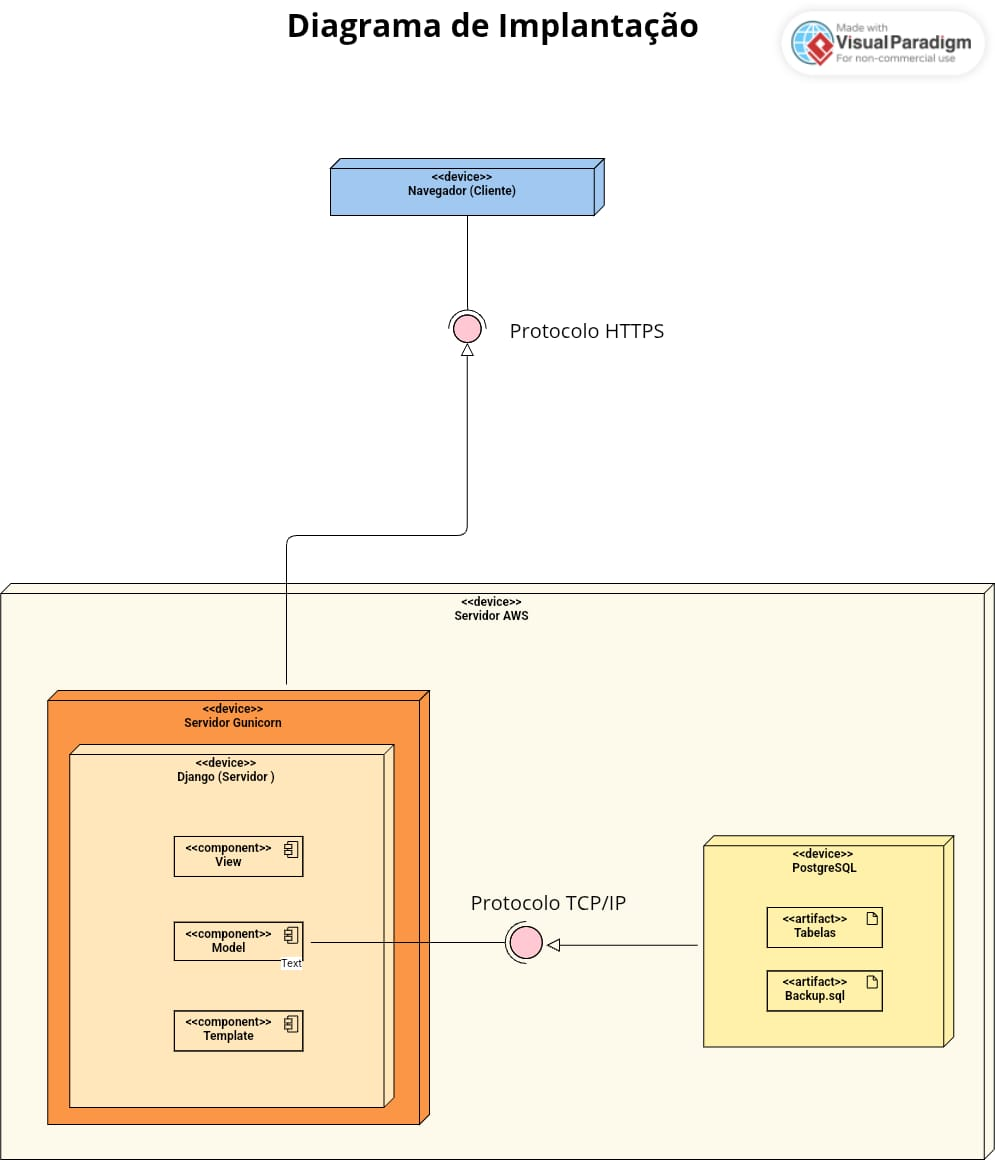
\includegraphics[width=\textwidth]{Diagrama de Implantação- Digitalização da Pousada.JPEG}
	\caption{Diagrama de Implantação desenvolvido no Online Visual-Paradigm}
	\label{fig:diagramaimplantação}
\end{figure}
\subsubsection{Diagrama de Componentes}
A Figura~\ref{fig:diagramacomponentes} mostra o funcionamento da arquitetura do sistema.

\begin{figure}[h!]
	\centering
	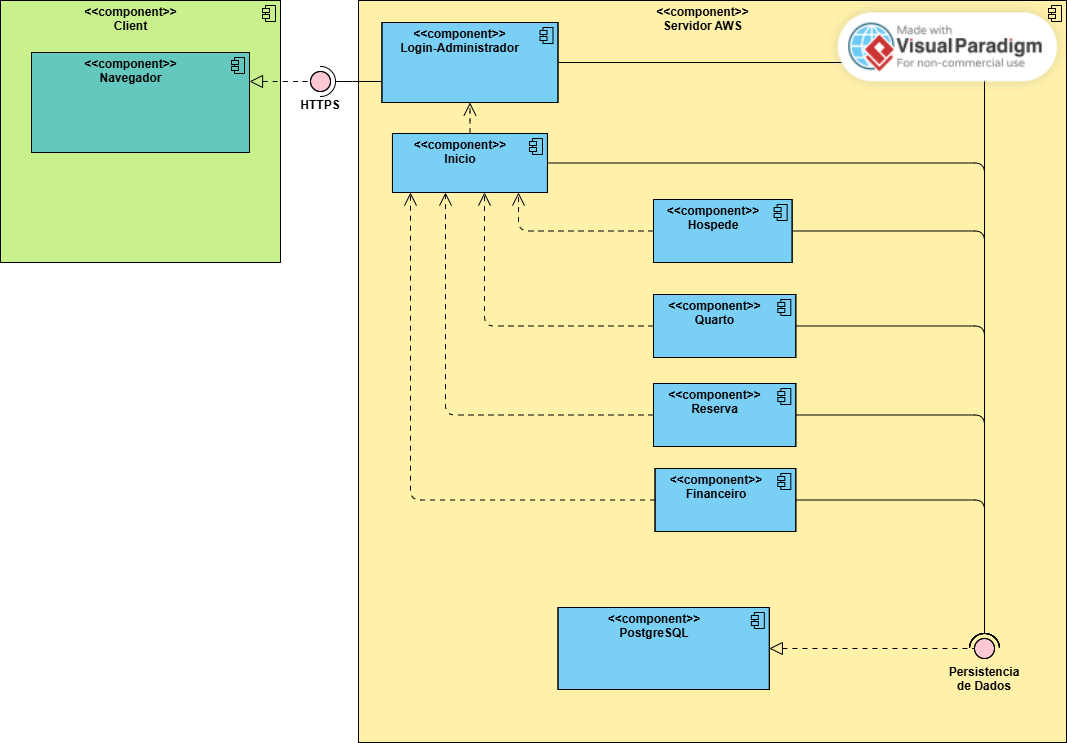
\includegraphics[width=\textwidth]{0406-Componentes.png}
	\caption{Diagrama de Componentes desenvolvido no Online Visual-Paradigm}
	\label{fig:diagramacomponentes}
\end{figure}


\section{Tecnologias}
O desenvolvimento do sistema da Pousada Chalés Água de Coco foi baseado na adoção de tecnologias modernas, acessíveis e amplamente utilizadas no mercado. A escolha dessas tecnologias teve como objetivo garantir robustez, escalabilidade, segurança e facilidade de manutenção. Nesta seção, são apresentadas as principais ferramentas e frameworks adotados, com ênfase no Django, framework principal da aplicação, além da infraestrutura de banco de dados e nuvem utilizada. Também são detalhados os motivos técnicos que justificam essas escolhas.
\subsection{Django}

O Django é um framework web de alto nível baseado em Python que oferece uma série de recursos que o tornam ideal para o desenvolvimento de sistemas como o nosso gerenciador de reservas de quartos~\cite{python}. Uma de suas principais vantagens é a rapidez no desenvolvimento, já que ele vem com diversas funcionalidades já prontas~\cite{django}.

\subsubsection{Front-end}

O desenvolvimento do Frond-end da aplicação Chalés Água de Coco se dá pela combinação de templates HTML associados a Views (Django) para gerar páginas dinâmicas. Os templates exibem essas informações de forma estruturada na interface do usuário, permitindo que elementos HTML sejam preenchidos com dados fornecidos pelo servidor, assim utilizando o padrão MTV.

O que facilita a manutenção e a escalabilidade do sistema. Isso é essencial em um sistema de reservas, que pode crescer em funcionalidades como calendário de disponibilidade, gestão de hóspedes, geração de relatórios, envio de notificações, entre outros.

\subsubsection{Back-end}

O desenvolvimento do back-end desta aplicação Django é baseada no padrão MTV, assim funcionando com manipulação de dados e lógica de negócio através das Views, que são responsáveis por processar requisições, acessar o banco de dados e enviar informações para os templates.

\subsubsection{Banco de Dados}

O Banco de Dados é o PostgreSQL, sendo um banco escalável e flexível, este SGBD pode suportar grandes volumes de dados e de usuários além de ser compatível com uma grande gama de linguagens de programação.
O PostgreSQL também é uma ótima opção por ser acessível, já que sua licença é livre, assim sem custos de licenciamento e a liberdade para modificar ou implementar o código-fonte da maneira que for necessária~\cite{postgresql}.

\subsection{Justificativa da Escolha}

A escolha do framework Django para o desenvolvimento do sistema da Pousada Chalés Água de Coco baseou-se em critérios técnicos, de segurança, escalabilidade e aderência às boas práticas de desenvolvimento web moderno. Django é um framework escrito em Python, que segue o padrão MTV, semelhante ao clássico MVC(Model-View-Controller), promovendo uma clara separação entre as camadas da aplicação ~\cite{python}.

\subsubsection{Justificativa Técnica}

Entre os diferenciais do Django, destacam-se o ORM nativo, que abstrai o uso de SQL e facilita a manipulação segura dos dados; o sistema integrado de autenticação e autorização, que oferece controle de acesso granular; e a proteção nativa contra ataques como SQL Injection, Cross-Site Scripting (XSS) e Cross-Site Request Forgery (CSRF). Esses recursos reduzem significativamente o tempo de desenvolvimento e aumentam a segurança da aplicação.
Além disso, o Django é um software de código aberto, com forte comunidade ativa, documentação completa e contínua evolução. Essa característica o torna ideal para projetos acadêmicos e corporativos, permitindo a entrega de soluções confiáveis e bem estruturadas~\cite{django}.

\subsubsection{Infraestrutura com AWS}
A escolha pela Amazon Web Services (AWS) como provedora da infraestrutura em nuvem está relacionada à sua capacidade de oferecer escalabilidade, disponibilidade e segurança~\cite{aws-doc}. Os recursos de computação elástica, gerenciamento de banco de dados, balanceamento de carga, armazenamento e backup são fundamentais para a operação de um sistema que lida com informações sensíveis de clientes e reservas.
A integração entre Django e AWS ocorre de forma transparente, possibilitando o uso de serviços como S3 (armazenamento de mídia), RDS (gerenciamento de banco de dados relacional) e CloudWatch (monitoramento), ampliando o potencial da aplicação e assegurando a continuidade do serviço com mínimo risco de falhas.


\section{Ferramentas de Apoio}
Durante o desenvolvimento do sistema da Pousada Chalés Água de Coco, foram empregadas diversas ferramentas que auxiliaram em diferentes etapas do projeto, desde a modelagem de dados e a construção da arquitetura até o controle de versões, documentação e comunicação entre os membros da equipe. A escolha dessas ferramentas foi guiada por critérios como acessibilidade, confiabilidade, funcionalidades oferecidas e integração com as tecnologias adotadas. A seguir, são descritas as principais ferramentas utilizadas e suas contribuições para o sucesso do projeto.
\subsection{GitHub}
O GitHub foi utilizado para controle de versão e colaboração durante o desenvolvimento do sistema. A plataforma permite armazenar e gerenciar o código-fonte, realizar revisões e integrar funcionalidades de forma eficiente. O GitHub facilitou a organização do fluxo de trabalho, o rastreamento de mudanças e a colaboração entre os membros da equipe, promovendo maior controle e transparência no ciclo de desenvolvimento~\cite{github-doc}.
\subsection{BRModelo}
O BRModelo foi utilizado para a modelagem lógica e relacional do banco de dados. A ferramenta oferece uma interface intuitiva para construção de diagramas entidade-relacionamento (DER), o que auxiliou na estruturação clara das tabelas, relacionamentos e chaves do sistema~\cite{brmodelo}. O uso do BRModelo contribuiu diretamente para a coerência e integridade do esquema de dados implementado no PostgreSQL.
\subsection{Visual Paradigm Online}
O Visual Paradigm Online foi utilizado na criação dos diagramas de Implantação e Componentes. Esta ferramenta auxiliou na documentação da arquitetura do sistema, contribuindo para uma melhor compreensão dos fluxos e interações entre os componentes~\cite{visual-paradigm}. A versão online possibilitou colaboração remota e armazenamento em nuvem, o que otimizou a produtividade da equipe.
\subsection{Latex}
O LaTeX foi utilizado na produção e formatação do trabalho acadêmico. Por meio de seu sistema de marcação, foi possível obter um alto nível de controle sobre a estrutura e apresentação do documento, garantindo consistência, qualidade e organização~\cite{latex-project}.

\subsection{Google Meet}
O Google Meet foi utilizado como plataforma de comunicação e realização de encontros virtuais da equipe ao longo do desenvolvimento do projeto~\cite{google-meet}. As reuniões periódicas possibilitaram a discussão de tarefas, alinhamento de prazos e entregas mais organizadas.

\section{Manutenibilidade}
A manutenibilidade do sistema de reservas para pousadas desenvolvido neste projeto é assegurada por meio de práticas estruturadas de engenharia de software, que facilitam a correção de erros, inclusão de novas funcionalidades e adaptação a futuras necessidades.

O sistema foi criado com uma arquitetura modular, respeitando os princípios de separação de responsabilidades. Isso permite que diferentes partes do sistema, como interface, regras de negócio e persistência de dados, sejam modificadas de forma independente, minimizando impactos colaterais e reduzindo o tempo de manutenção.

Além disso, foram adotados padrões de codificação consistentes e bem documentados, com o intuito de facilitar a leitura e compreensão do código por outros desenvolvedores. Esses padrões promovem a reutilização e a extensibilidade do sistema.

A utilização do sistema de controle de versão Git, em conjunto com a plataforma GitHub, possibilita o rastreamento detalhado de alterações, revisão de código e colaboração eficaz entre os membros da equipe~\cite{github-doc}. Isso garante maior controle sobre o histórico de desenvolvimento e facilita a identificação e resolução de falhas.

A aplicação também contará com testes automatizados, cobrindo os principais fluxos da aplicação, como testes unitários para funções críticas e testes de integração entre os módulos.

Por fim, o projeto segue um ciclo de desenvolvimento bem definido, com etapas de planejamento, codificação, testes, implantação e manutenção. Essa abordagem estruturada proporciona maior previsibilidade, qualidade e agilidade na evolução contínua da aplicação, assegurando sua longevidade e adaptabilidade.

\section{Segurança, Privacidade e Legislação}

A segurança da informação, a proteção de dados e o cumprimento das normas legais foram diretrizes centrais na concepção do sistema de reservas da Pousada Chalés Água de Coco. Para tanto, foram adotadas boas práticas de desenvolvimento seguro, recursos nativos do framework Django e medidas alinhadas à Lei Geral de Proteção de Dados (LGPD – Lei nº 13.709/2018).

\subsection{Segurança da Aplicação}

O framework Django oferece proteção automática contra ameaças comuns da web, como injeção de SQL, execução remota de código, Cross-Site Scripting (XSS) e falsificação de requisições entre sites (CSRF)~\cite{django}. Além disso, foram implementadas as seguintes práticas:

Sistema de autenticação e autorização: Controle de acesso baseado em permissões, exigência de credenciais válidas e proteção de páginas sensíveis por autenticação obrigatória.

Proteção contra CSRF: Utilização de tokens em requisições POST, garantindo que apenas usuários legítimos possam executar ações críticas.

Escapamento automático de HTML (XSS): O mecanismo de templates evita a execução de scripts maliciosos.
Armazenamento seguro de senhas: Utilização de algoritmos modernos de hash, como PBKDF2, inviabilizando a recuperação das senhas mesmo em caso de vazamento.

Gerenciamento seguro de sessões: Identificadores criptografados, proteção contra falsificação e expiração automática de sessões inativas.


\subsection{Segurança na Comunicação}

Todas as comunicações entre cliente e servidor são realizadas via HTTPS, com uso de certificado SSL/TLS. O certificado foi emitido por uma autoridade certificadora confiável, após validação de domínio e instalação no servidor da AWS~\cite{aws-doc}. A criptografia das conexões assegura a confidencialidade, integridade e autenticidade dos dados transmitidos.
A aplicação redireciona automaticamente requisições HTTP para HTTPS e adiciona cabeçalhos HTTP de segurança, prevenindo de possíveis ataques.


\subsubsection{Conformidade com a LGPD}
Para atender aos princípios da LGPD, o sistema foi projetado com foco na coleta mínima de dados, na transparência quanto ao uso das informações e no controle por parte do titular dos dados. São assegurados os seguintes direitos:

Solicitação de remoção de dados pessoais;

Alteração de consentimento previamente fornecido;

Acesso claro às finalidades do tratamento dos dados.

Além disso, os dados são armazenados de forma segura e submetidos a backups regulares em ambiente de nuvem, garantindo resiliência e conformidade com os princípios de segurança, prevenção e responsabilização da LGPD~\cite{lgpd}.


\section{Modelagem do Banco de Dados}
A modelagem do banco de dados é uma etapa fundamental no desenvolvimento de sistemas de informação, pois define a estrutura lógica e relacional para o armazenamento e manipulação dos dados. No sistema da Pousada Chalés Água de Coco, a modelagem foi realizada com foco na integridade dos dados, normalização e clareza nos relacionamentos entre as entidades.

Utilizando a ferramenta BRModelo, foram construídos o Modelo Entidade Relacionamento (MER) e o Diagrama Entidade Relacionamento (DER), os quais serviram como base para a implementação do banco de dados relacional no PostgreSQL. Esses diagramas ajudam a visualizar as entidades principais do sistema, como hóspedes, reservas, quartos, bem como os vínculos entre elas, garantindo coerência e consistência no projeto de dados.
\subsection{Modelo Entidade-Relacionamento - MER}

A Figura~\ref{fig:mer} mostra o Modelo Entidade-Relacionamento (MER) do sistema.

\begin{figure}[h!]
	\centering
	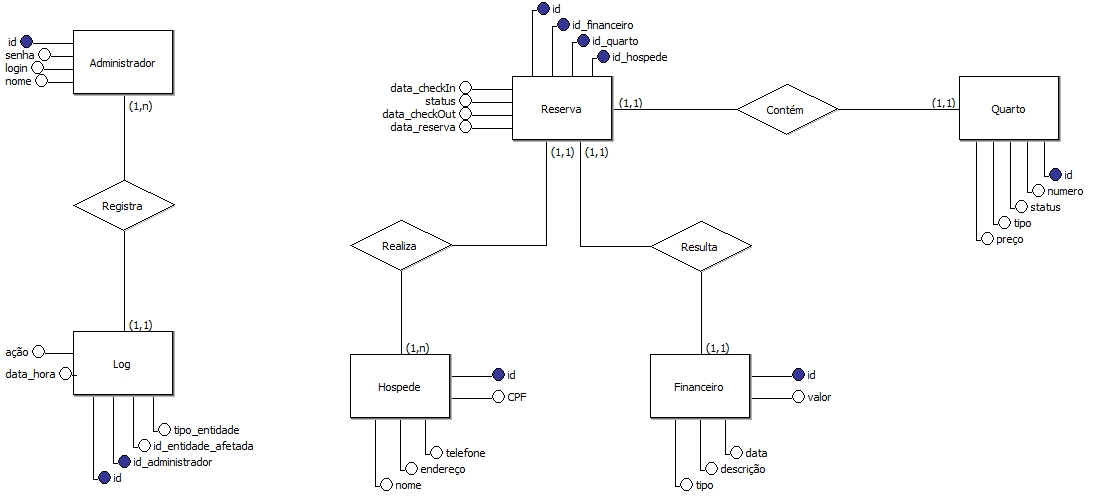
\includegraphics[width=\textwidth]{0406-MER.jpg}
	\caption{Modelo Entidade-Relacionamento (MER) desenvolvido no brModelo}
	\label{fig:mer}
\end{figure}
\subsection{Diagrama Entidade-Relacionamento - DER}
A Figura~\ref{fig:der} mostra o Diagrama Entidade-Relacionamento (DER) do sistema.

\begin{figure}[H]
	\centering
	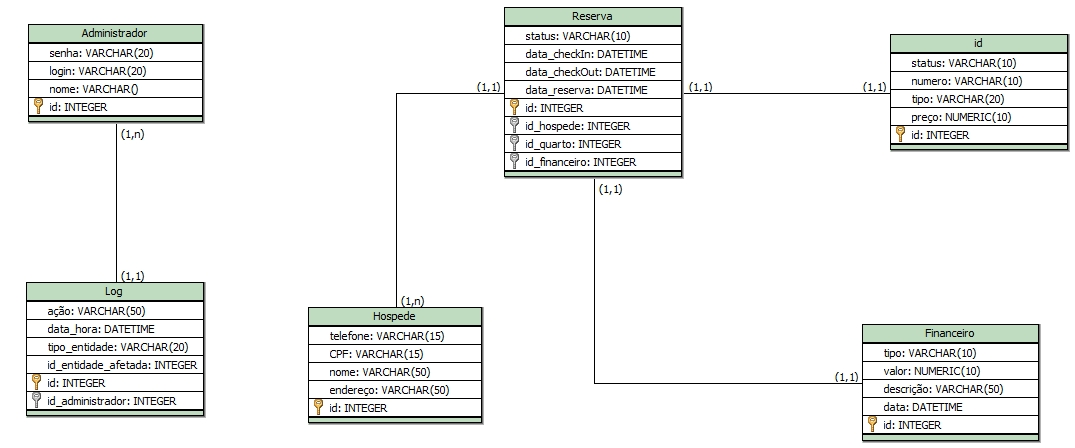
\includegraphics[width=\textwidth]{0406-DER.jpg}
	\caption{Diagrama Entidade-Relacionamento (DER) desenvolvido no brModelo}
	\label{fig:der}
\end{figure}


\section{Entregas}
O desenvolvimento do sistema seguiu um cronograma baseado em entregas parciais, cada uma representando uma etapa importante na evolução do projeto. Essas entregas permitiram o acompanhamento contínuo do progresso, validação das funcionalidades e documentação formal de todas as fases do trabalho. A seguir, são descritas as principais entregas realizadas ao longo do semestre, com seus respectivos objetivos e resultados.
\subsection{Desenvolvimento de um Tema - 08/04}

Nesta etapa inicial, foi definido o tema central do projeto: o desenvolvimento de um sistema web para automatizar os processos administrativos da pousada Chalés Água de Coco. A escolha foi baseada em uma demanda real identificada junto ao empreendimento, permitindo alinhar os objetivos acadêmicos com a solução de um problema concreto.

\subsection{Desenho da Aplicação - 29/04}

Foi elaborada a arquitetura do sistema utilizando os diagramas UML de Componentes e de Implantação, utilizando o padrão MTV (Model-Template-View) do framework Django. Nessa fase, também foi realizada a modelagem inicial do banco de dados relacional utilizando o PostgreSQL

\subsection{Prova de Conceito - 20/05}

Na etapa da prova de conceito, foi desenvolvido um sistema funcional de cadastro de hóspedes, com a aplicação já hospedada na infraestrutura da Amazon Web Services (AWS). Nesta versão inicial, foi implementado um CRUD completo (Create, Read, Update, Delete) utilizando o banco de dados relacional PostgreSQL, gerenciado por meio do ORM nativo do Django. Essa entrega permitiu validar a viabilidade técnica da solução, testar a integração entre as camadas da aplicação e comprovar o funcionamento do ambiente de produção na nuvem.

\subsection{Análise e Documentação - 10/06}

Nesta etapa, foi realizada a entrega da documentação referente ao Projeto de Conclusão de Curso (PCC), contendo toda a análise do problema, justificativas, objetivos, levantamento de requisitos, arquitetura do sistema, escolha das tecnologias e desenvolvimento. A documentação formaliza todas as etapas do projeto, desde sua concepção até a implementação da solução proposta, servindo como registro técnico e acadêmico do trabalho desenvolvido.

\subsection{Produto Mínimo Viável - 24/06}

O Produto Mínimo Viável (MVP) entregue contempla as funcionalidades essenciais do sistema, focando na gestão de hóspedes, acomodações e reservas. Essas funcionalidades já permitem à pousada Chalés Água de Coco substituir o controle manual por um sistema digital centralizado e acessível. A parte de controle financeiro, embora planejada, será desenvolvida em uma fase posterior, prevista para o próximo semestre.


\chapter{Viabilidade Financeira}
Visando a viabilidade financeira do desenvolvimento da aplicação de gestão de reservas de quarto, conduzimos um estudo dos custos necessários e produzimos relatórios referentes a diferentes cenários. Os dados utilizados no estudo são concretos e retirados de fontes seguras, nos ajudando a visualizar a factibilidade do projeto e ter melhor percepção para a tomada de decisões estratégicas.

\section{Custos}
\subsection{Custo Estrutural}

A parte de custos por estrutura está divida entre Equipamentos e Serviços, que diz respeito aos equipamentos e serviços necessários para que cada colaborador do time consiga desempenhar suas funções. E Infraestrutura, que aborda os custos relativos a sustentação do sistema.

Considerando que a equipe trabalha no regime home office e utiliza seus próprios equipamentos, entendemos os gastos como nulos. Partindo assim para tarifas referentes a energia e internet~\cite{anatel-anexo}.
Já nos custos indicados na parte de infraestrutura foram considerados nulos pois o sistema será desenvolvido utilizando serviços gratuito (lembrando que essa análise se trata de uma estimativa, e que caso haja alguma mudança significativa no projeto ou necessidade de serviços pagos, esses custos podem mudar)~\cite{enel-tarifa}.

\begin{table}[H]
	\centering
	\caption{Resumo dos custos de Equipamentos e Serviços}
	\label{tab:equipamentos-servicos}
	\begin{tabular}{|l|c|r|r|r|}
		\hline
		\textbf{Itens} & \textbf{Quantidade} & \textbf{Custo mensal} & \textbf{Total 4 meses} & \textbf{Total 9 meses} \\
		\hline
		Notebooks & 6 & R\$ 0,00 & R\$ 0,00 & R\$ 0,00 \\
		\hline
		Roteadores & 6 & R\$ 0,00 & R\$ 0,00 & R\$ 0,00 \\
		\hline
		Internet (Assinatura) & 6 & R\$ 114,97 & R\$ 2.759,28 & R\$ 6.208,38 \\
		\hline
		Eletricidade (Fatura) & 6 & R\$ 3,44 & R\$ 82,56 & R\$ 185,76 \\
		\hline
		\textbf{Total} & 24 & R\$ 118,41 & R\$ 2.841,84 & R\$ 6.394,14 \\
		\hline
	\end{tabular}
	\fonte{Elaborado pelos autores}
\end{table}

\begin{table}[H]
	\centering
	\caption{Resumo dos custos de Infraestrutura}
	\label{tab:infraestrutura}
	\begin{tabular}{|l|l|r|r|r|}
		\hline
		\textbf{Tipo} & \textbf{Serviço} & \textbf{Mensal} & \textbf{Total 4 meses} & \textbf{Total 9 meses} \\
		\hline
		Proxy Reverso & Servidor Nginx & R\$ 0,00 & R\$ 0,00 & R\$ 0,00 \\
		\hline
		Aplicação & Servidor Gunicorn & R\$ 0,00 & R\$ 0,00 & R\$ 0,00 \\
		\hline
		Framework Web & Servidor Django & R\$ 0,00 & R\$ 0,00 & R\$ 0,00 \\
		\hline
		Banco de Dados & PostgreSQL & R\$ 0,00 & R\$ 0,00 & R\$ 0,00 \\
		\hline
		Hospedagem & AWS & R\$ 0,00 & R\$ 0,00 & R\$ 0,00 \\
		\hline
		\textbf{Total} & & R\$ 0,00 & R\$ 0,00 & R\$ 0,00 \\
		\hline
	\end{tabular}
	\fonte{Elaborado pelos autores.}
\end{table}

\subsection{Custo Mão de Obra}

Na imagem a seguir temos uma tabela detalhada com os custos referentes a mão de obra do desenvolvimento do projeto. 
Na primeira coluna temos a especificação dos papéis de cada profissional, em seguida quantidade de pessoas por cargo, horas trabalhadas ao dia e dias trabalhados ao mês(média).
Também podemos checar o preço por hora de cada profissional, assim finalizamos com as estimativas de custo mensal, total 4 meses (correspondente ao tempo em que a equipe já trabalhou no projeto até então) e projeção 9 meses (correspondente ao tempo total estimado de projeto).

% Tabela 1 - Dados de horas
\begin{table}[H]
	\centering
	\caption{Quantidade e horas trabalhadas por função}
	\label{tab:mao-de-obra-horas}
	\adjustbox{max width=\textwidth}{
		\begin{tabular}{|>{\RaggedRight\arraybackslash}p{5.5cm}|c|c|c|c|}
			\hline
			\textbf{Função} & \textbf{Quantidade} & \textbf{Horas/Dia} & \textbf{Dias/Mês} & \textbf{Total de Horas/Mês} \\
			\hline
			Analista de Cronograma (PMO)     & 1 & 6 & 22 & 132 \\
			\hline
			Engenheiro de Dados (DBA)        & 1 & 6 & 22 & 132 \\
			\hline
			Analista de Documentação         & 1 & 6 & 22 & 132 \\
			\hline
			Gerente de Projeto (PM)          & 1 & 6 & 22 & 132 \\
			\hline
			Desenvolvedor Front-End          & 1 & 6 & 22 & 132 \\
			\hline
			Desenvolvedor Back-End           & 1 & 6 & 22 & 132 \\
			\hline
			\textbf{Total Mão de Obra}       & 6 & 36 & 132 & 792 \\
			\hline
		\end{tabular}
	}
	\fonte{Elaborado pelos autores.}
\end{table}

\begin{table}[H]
	\centering
	\caption{Custos por função}
	\label{tab:mao-de-obra-custos}
	\adjustbox{max width=\textwidth}{
		\begin{tabular}{|>{\RaggedRight\arraybackslash}p{5.5cm}|r|r|r|r|}
			\hline
			\textbf{Função} & \textbf{Custo Hora (R\$)} & \textbf{Custo Mensal (R\$)} & \textbf{Total 4 meses (R\$)} & \textbf{Total 9 meses (R\$)} \\
			\hline
			Analista de Cronograma (PMO)     & 16,00 & 2.112,00 & 8.448,00 & 19.008,00 \\
			\hline
			Engenheiro de Dados (DBA)        & 13,00 & 1.716,00 & 6.864,00 & 15.444,00 \\
			\hline
			Analista de Documentação         & 15,00 & 1.980,00 & 7.920,00 & 17.820,00 \\
			\hline
			Gerente de Projeto (PM)          & 16,00 & 2.112,00 & 8.448,00 & 19.008,00 \\
			\hline
			Desenvolvedor Front-End          & 13,00 & 1.716,00 & 6.864,00 & 15.444,00 \\
			\hline
			Desenvolvedor Back-End           & 13,00 & 1.716,00 & 6.864,00 & 15.444,00 \\
			\hline
			\textbf{Total Mão de Obra}       & 86,00 & 11.352,00 & 45.408,00 & 102.168,00 \\
			\hline
		\end{tabular}
	}
	\fonte{Elaborado pelos autores.}
\end{table}

\subsection{Custo Total}

Na imagem a seguir temos a junção dos custos por mão de obra e custos por estrutura, sendo visualizadas em 3 períodos diferentes:
Custo Mensal - Referente a gastos de um único mês.
Custo Total (4 meses) - Custos referentes aos meses que foram trabalhados até a data de escrita deste texto.
Custo Total (9 meses) - Custos referentes ao total de meses programado para a realização do projeto.

\begin{table}[h!]
	\centering
	\caption{Custo Total por Categoria}
	\label{tab:custo-total}
	\adjustbox{max width=\textwidth}{
		\begin{tabular}{|l|r|r|r|}
			\hline
			\textbf{Categoria} & \textbf{Custo Mensal (R\$)} & \textbf{Custo Total (4 meses) (R\$)} & \textbf{Custo Total (9 meses) (R\$)} \\
			\hline
			Mão de Obra & 11.352,00 & 45.408,00 & 102.168,00 \\
			Estrutura   & 710,46    & 2.841,84  & 6.394,14 \\
			\hline
			\textbf{Total} & 12.062,46 & 48.249,84 & 108.562,14 \\
			\hline
		\end{tabular}
	}
	\fonte{Elaborado pelos autores.}
\end{table}

\section{Cenários}

\subsection{Cenário Otimista}

Na imagem a seguir podemos observar a projeção construída pela equipe de um cenário otimista, levando em consideração os custos já apresentados anteriormente de mão de obra e estrutura. Podemos observar que de acordo com essa projeção, o ponto de equilíbrio será alcançado por volta de 6 meses.

\begin{figure}[H]
	\centering
	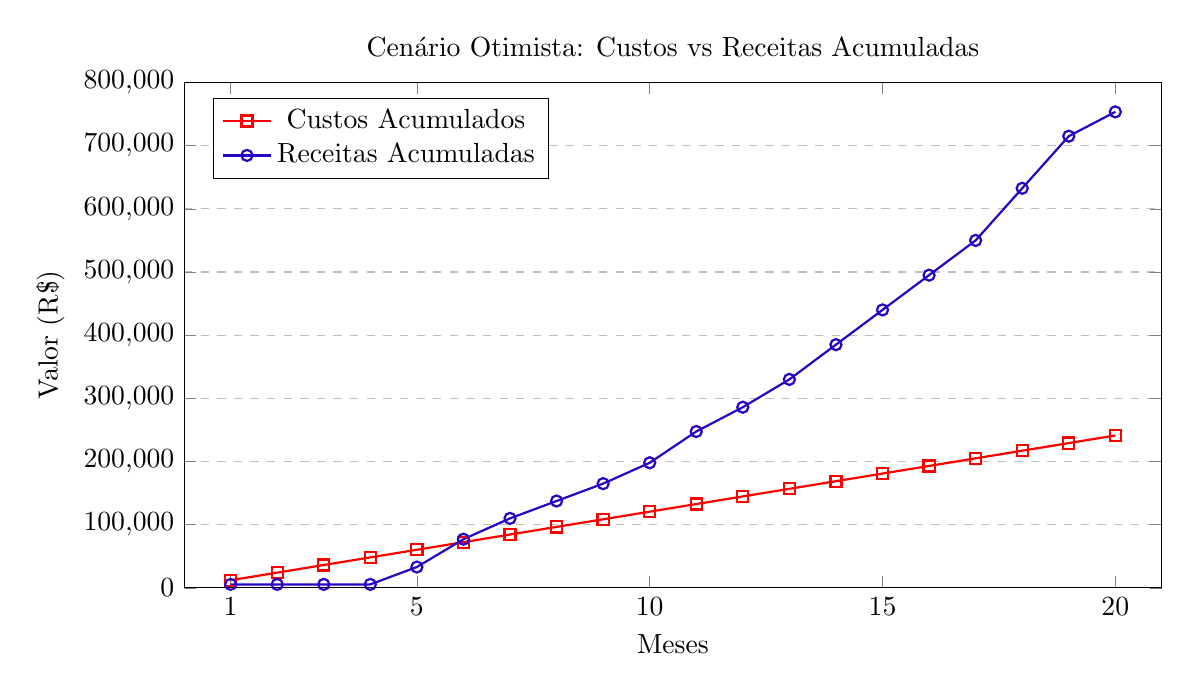
\begin{tikzpicture}
		\begin{axis}[
			title={Cenário Otimista: Custos vs Receitas Acumuladas},
			xlabel={Meses},
			ylabel={Valor (R\$)},
			xmin=0, xmax=21,
			ymin=0, ymax=800000,
			xtick={1,5,10,15,20},
			ytick={0,100000,200000,300000,400000,500000,600000,700000,800000},
			legend pos=north west,
			ymajorgrids=true,
			grid style=dashed,
			width=14cm,
			height=8cm,
			scaled y ticks = false,
			ticklabel style={/pgf/number format/fixed},
			]
			
			% Dados Custos Acumulados
			\addplot[
			color=red,
			mark=square,
			thick,
			]
			coordinates {
				(1,12062.46)
				(2,24124.92)
				(3,36187.38)
				(4,48249.84)
				(5,60312.30)
				(6,72374.76)
				(7,84437.22)
				(8,96499.68)
				(9,108562.14)
				(10,120624.60)
				(11,132687.06)
				(12,144749.52)
				(13,156811.98)
				(14,168874.44)
				(15,180936.90)
				(16,192999.36)
				(17,205061.82)
				(18,217124.28)
				(19,229186.74)
				(20,241249.20)
			};
			
			% Dados Receitas Acumuladas
			\addplot[
			color=blue,
			mark=o,
			thick,
			]
			coordinates {
				(1,5500)
				(2,5500)
				(3,5500)
				(4,5500)
				(5,33000)
				(6,77000)
				(7,110000)
				(8,137500)
				(9,165000)
				(10,198000)
				(11,247500)
				(12,286000)
				(13,330000)
				(14,385000)
				(15,440000)
				(16,495000)
				(17,550000)
				(18,632500)
				(19,715000)
				(20,753500)
			};
			
			\legend{Custos Acumulados, Receitas Acumuladas}
		\end{axis}
	\end{tikzpicture}
	\caption{Comparação dos custos e receitas acumuladas no cenário otimista}
	\label{fig:custo-receita-otimista}
\end{figure}


\subsection{Cenário Pessimista}

Na imagem a seguir podemos observar a projeção construída pela equipe de um cenário pessimista, levando em consideração os custos já apresentados anteriormente de mão de obra e estrutura. Podemos observar que de acordo com essa projeção, o ponto de equilíbrio será alcançado por volta de 20 meses.

\begin{figure}[H]
	\centering
	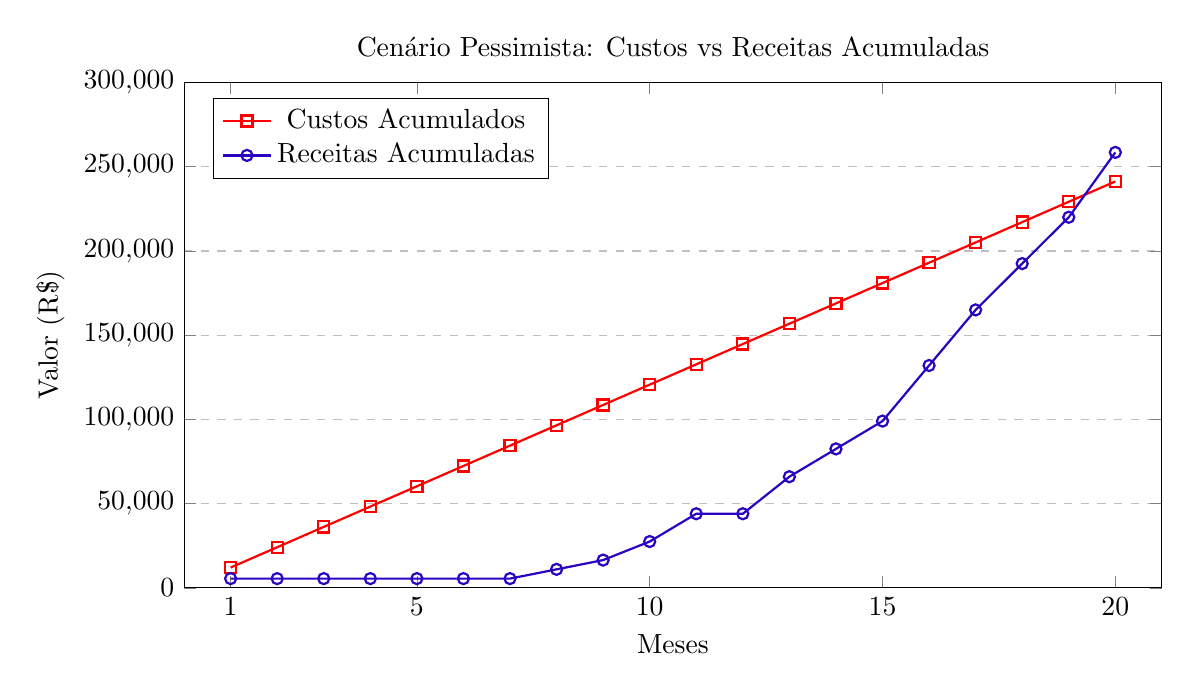
\begin{tikzpicture}
		\begin{axis}[
			title={Cenário Pessimista: Custos vs Receitas Acumuladas},
			xlabel={Meses},
			ylabel={Valor (R\$)},
			xmin=0, xmax=21,
			ymin=0, ymax=300000,
			xtick={1,5,10,15,20},
			ytick={0,50000,100000,150000,200000,250000,300000},
			legend pos=north west,
			ymajorgrids=true,
			grid style=dashed,
			width=14cm,
			height=8cm,
			scaled y ticks = false,
			ticklabel style={/pgf/number format/fixed},
			]
			
			% Dados Custos Acumulados
			\addplot[
			color=red,
			mark=square,
			thick,
			]
			coordinates {
				(1,12062.46)
				(2,24124.92)
				(3,36187.38)
				(4,48249.84)
				(5,60312.30)
				(6,72374.76)
				(7,84437.22)
				(8,96499.68)
				(9,108562.14)
				(10,120624.60)
				(11,132687.06)
				(12,144749.52)
				(13,156811.98)
				(14,168874.44)
				(15,180936.90)
				(16,192999.36)
				(17,205061.82)
				(18,217124.28)
				(19,229186.74)
				(20,241249.20)
			};
			
			% Dados Receitas Acumuladas
			\addplot[
			color=blue,
			mark=o,
			thick,
			]
			coordinates {
				(1,5500)
				(2,5500)
				(3,5500)
				(4,5500)
				(5,5500)
				(6,5500)
				(7,5500)
				(8,11000)
				(9,16500)
				(10,27500)
				(11,44000)
				(12,44000)
				(13,66000)
				(14,82500)
				(15,99000)
				(16,132000)
				(17,165000)
				(18,192500)
				(19,220000)
				(20,258500)
			};
			
			\legend{Custos Acumulados, Receitas Acumuladas}
		\end{axis}
	\end{tikzpicture}
	\caption{Comparação dos custos e receitas acumuladas no cenário pessimista}
	\label{fig:custo-receita-pessimista}
\end{figure}


\subsection{Cenário Realista}

Na imagem a seguir podemos observar a projeção construída pela equipe de um cenário realista, levando em consideração os custos já apresentados anteriormente de mão de obra e estrutura. Podemos observar que de acordo com essa projeção, o ponto de equilíbrio será alcançado por volta de 15 meses.

\begin{figure}[H]
	\centering
	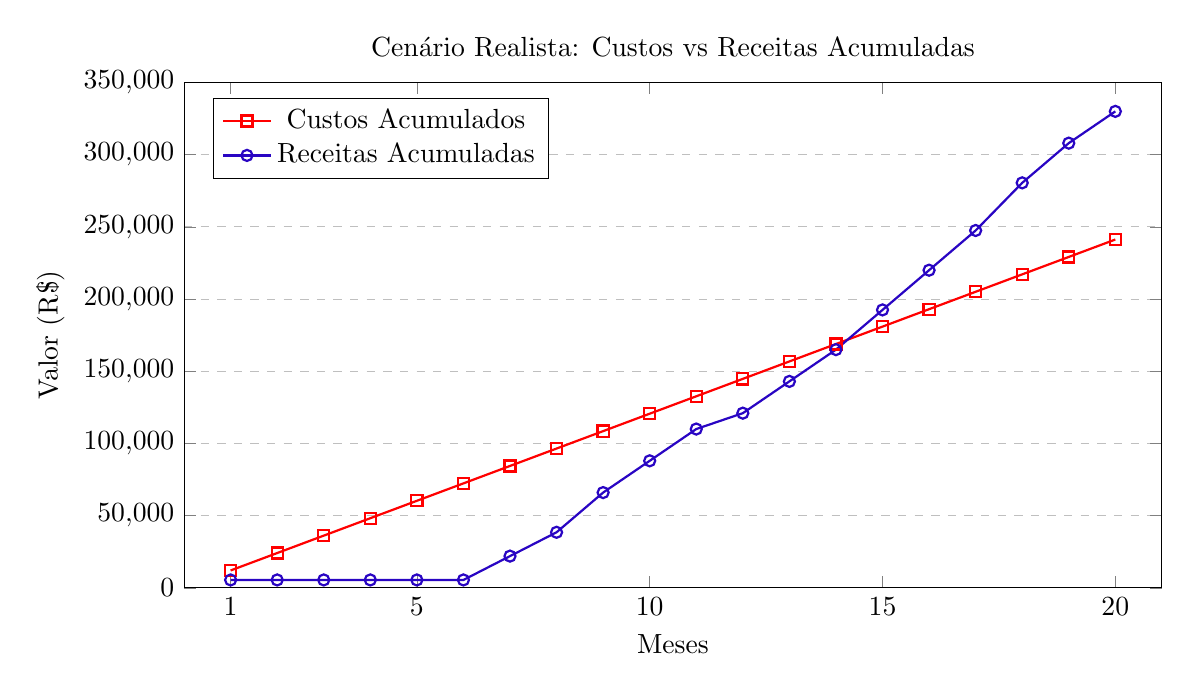
\begin{tikzpicture}
		\begin{axis}[
			title={Cenário Realista: Custos vs Receitas Acumuladas},
			xlabel={Meses},
			ylabel={Valor (R\$)},
			xmin=0, xmax=21,
			ymin=0, ymax=350000,
			xtick={1,5,10,15,20},
			ytick={0,50000,100000,150000,200000,250000,300000,350000},
			legend pos=north west,
			ymajorgrids=true,
			grid style=dashed,
			width=14cm,
			height=8cm,
			scaled y ticks = false,
			ticklabel style={/pgf/number format/fixed},
			]
			
			% Dados Custos Acumulados
			\addplot[
			color=red,
			mark=square,
			thick,
			]
			coordinates {
				(1,12062.46)
				(2,24124.92)
				(3,36187.38)
				(4,48249.84)
				(5,60312.30)
				(6,72374.76)
				(7,84437.22)
				(8,96499.68)
				(9,108562.14)
				(10,120624.60)
				(11,132687.06)
				(12,144749.52)
				(13,156811.98)
				(14,168874.44)
				(15,180936.90)
				(16,192999.36)
				(17,205061.82)
				(18,217124.28)
				(19,229186.74)
				(20,241249.20)
			};
			
			% Dados Receitas Acumuladas
			\addplot[
			color=blue,
			mark=o,
			thick,
			]
			coordinates {
				(1,5500)
				(2,5500)
				(3,5500)
				(4,5500)
				(5,5500)
				(6,5500)
				(7,22000)
				(8,38500)
				(9,66000)
				(10,88000)
				(11,110000)
				(12,121000)
				(13,143000)
				(14,165000)
				(15,192500)
				(16,220000)
				(17,247500)
				(18,280500)
				(19,308000)
				(20,330000)
			};
			
			\legend{Custos Acumulados, Receitas Acumuladas}
		\end{axis}
	\end{tikzpicture}
	\caption{Comparação dos custos e receitas acumuladas no cenário realista}
	\label{fig:custo-receita-realista}
\end{figure}

\chapter{Considerações Finais}

O desenvolvimento do sistema web para a pousada Chalés Água de Coco representa uma resposta prática e eficiente à necessidade de modernização enfrentada por pequenos empreendimentos do setor de hospitalidade. Ao longo do projeto, foi possível identificar fragilidades nos métodos tradicionais utilizados para gestão de hóspedes, reservas e finanças — especialmente aqueles baseados em planilhas eletrônicas — que, embora populares, oferecem baixa escalabilidade, alto risco de erro e pouca integração entre processos.

Através de uma parceria direta com os responsáveis pela pousada, foi possível realizar um levantamento detalhado dos requisitos do sistema, o que permitiu construir uma solução personalizada, centrada nas reais necessidades operacionais do negócio. O uso do framework Django, aliado à infraestrutura da Amazon Web Services (AWS), proporcionou uma arquitetura robusta, segura e escalável, capaz de sustentar a aplicação tanto em seu estágio inicial quanto em futuras evoluções.

Além da automatização das principais funções administrativas da pousada, como o controle de reservas e a organização dos dados financeiros, o sistema promoveu melhorias significativas na usabilidade, no acesso remoto às informações e na geração de relatórios gerenciais. Com isso, o projeto atendeu plenamente aos seus objetivos, oferecendo uma ferramenta funcional, acessível via internet e com grande potencial de impacto na rotina de trabalho da pousada.

O projeto também demonstrou, na prática, a aplicabilidade dos conhecimentos adquiridos ao longo do curso, abrangendo aspectos de análise de requisitos, modelagem de dados, desenvolvimento back-end e front-end, segurança da informação e implantação em ambiente de nuvem. Trata-se, portanto, de um produto tecnológico que, além de resolver uma demanda real, reforça a importância da tecnologia na transformação digital de pequenos negócios.


%
% ----------------------------------------------------------
% Finaliza a parte no bookmark do PDF
% para que se inicie o bookmark na raiz
% e adiciona espaço de parte no Sumário
% ----------------------------------------------------------
\phantompart

% ---
% Conclusão
% ---
\chapter{Conclusão}
% ---

Este Projeto de Conclusão de Curso teve como propósito desenvolver um sistema web para automatizar os processos administrativos da pousada Chalés Água de Coco, promovendo uma solução moderna e eficiente em substituição ao modelo tradicional baseado em planilhas. O sistema entregue oferece recursos essenciais para a gestão de hóspedes, reservas, acomodações e controle financeiro, consolidando-se como uma plataforma completa e adaptada à realidade da pousada.

A aplicação da arquitetura MTV com o framework Django, a adoção de práticas seguras de desenvolvimento e o uso da infraestrutura em nuvem da AWS contribuíram para a construção de um sistema robusto e escalável, capaz de oferecer alto desempenho e disponibilidade. A utilização de tecnologias amplamente reconhecidas no mercado assegura não apenas a qualidade técnica do sistema, mas também sua viabilidade para expansão futura.

Como resultado, a pousada passa a contar com uma ferramenta que facilita a tomada de decisões, minimiza falhas operacionais e melhora a organização das informações. O projeto também evidencia como soluções de baixo custo e alto impacto podem ser desenvolvidas e aplicadas em pequenos negócios, promovendo inovação e melhoria contínua.


% ----------------------------------------------------------
% ELEMENTOS PÓS-TEXTUAIS
% ----------------------------------------------------------
\postextual
% ----------------------------------------------------------

% ----------------------------------------------------------
% Referências bibliográficas
% ----------------------------------------------------------
\bibliographystyle{abntex2-alf}
\bibliography{referencias}

% ----------------------------------------------------------
% Glossário
% ----------------------------------------------------------
%
% Consulte o manual da classe abntex2 para orientações sobre o glossário.
%
%\glossary

% ----------------------------------------------------------
% Apêndices
% ----------------------------------------------------------

% ---
% Inicia os apêndices
% ---
\begin{apendicesenv}

% Imprime uma página indicando o início dos apêndices
\partapendices

% ----------------------------------------------------------
\chapter{Diário de Bordo}
% ----------------------------------------------------------


\section{1° SEMANA}
Período: 25/03/2025 a 01/04/2025.

Nessa semana, com os membros da equipe definidos, iniciamos nossas atividades para o desenvolvimento do projeto da disciplina de Projeto de Extensão Integrado I. Assim, essa semana criamos um grupo na plataforma Whatsapp para estabelecermos nossa comunicação e facilitar o levantamento de possíveis temas para discutirmos em sala. Assim, no dia 01/04/2025 analisamos os parceiros disponíveis e a suas principais necessidades e optamos por desenvolver uma aplicação web para a empresa Pousada Chalés Água de Coco. 

\section{2° SEMANA}
Período: 01/04/2025 a 08/04/2025.

Durante essa semana aprofundamos nosso conhecimento sobre a empresa parceira escolhida, entendo sua principal necessidade: automatização dos serviços de gestão.
Definimos que iremos desenvolver uma aplicação web de gestão para a proprietária com o objetivo de facilitar e otimizar a administração do negócio. A partir disso, também definimos nosso MVP (Produto Mínimo Viável), levando em consideração nossa capacidade técnica e os serviços da pousada. Preenchemos a primeira planilha de avaliação do grupo e auto-avaliação. Por fim, nos preparamos para apresentar a nossa escolha de tema para o professor orientador, realizada no dia 08/04, na qual também apresentamos nosso MVP.
Funcionalidade MVP: Gestão de Reservas e Check-in/Check-out. 	


\section{3° SEMANA}
Período: 08/04/2025 a 15/04/2025.

Nesta semana começamos efetivamente as tarefas associadas ao desenvolvimento do nosso projeto. Foram elas:
- Definimos a metodologia de gestão de projeto Scrum. Usamos como base para  nossa escolha: experiências práticas/ conhecimento prévio da ferramenta, isto é, familiaridade. 
- Definimos a função de cada membro da equipe:
Anna Julia: Analista de Cronograma/ PMO.
Guilherme Akio: Engenheiro de Dados/ Administrador de Banco de Dados.
Guilherme Bittencourt: Analista de Documentação/Arquiteto de Software.
Kelly Radchelle: Gerente de Projeto.
Rafael Teixeira: Desenvolvedor Frontend.
Ricardo Carriel: Desenvolvedor Backend.
- Criamos nosso arquivo no ProjectLibre, adicionamos os principais marcos do projeto e os recursos humanos.
- Criamos nossa documentação LateX e fizemos as primeiras alterações no arquivo.
- Iniciamos o levantamento dos requisitos funcionais do MVP.


\section{4° SEMANA}
Período: 15/04/2025 a 22/04/2025.

Nesta semana foram realizadas as tarefas e discussões para iniciarmos o desenvolvimento do desenho da nossa aplicação:
Analisamos os requisitos funcionais levantados e definimos os requisitos não funcionais essenciais da nossa aplicação.
E definimos as plataformas e tecnologias que iremos usar.


\section{5° SEMANA}
Período: 22/04/2025 a 29/04/2025.

Essa semana foram desenvolvidas atividades ligadas ao desenvolvimento da prova de conceito. Foram elas:
- Documentação dos Casos de Uso - Kelly
- Documentação dos Diagramas de Caso de Uso -Guilherme Bittencourt.
Reunião via Google Meet na qual foi discutido o desenho da aplicação com todos os membros da equipe.
- Criação do Diagrama de Componentes -Guilherme Bittencourt.
- Criação do Diagrama de Implantação -Kelly Radchelle.
- Apresentação do Desenho da Aplicação - Guilherme Bittencourt, Guilherme Akio, Rafael Teixeira, Anna Julia e Ricardo Carriel.

\section{6° SEMANA}
Período: 29/04/2025 a 06/05/2025.

Após a entrega da prova de conceito na semana anterior os diagramas apresentados foram editados, corrigindo os pontos levantados 
pelo professor orientador. 
- Alterações no diagrama de componentes: Guilherme Bittencourt.
- Alterações no diagrama de implantação: Kelly.
- Criação do MER:Guilherme Bittencourt.
- Criação do repositório Git para versionamento da aplicação: Guilherme Bittencourt.
- Levantamento das regras de negócio e requisitos com a proprietária:  Kelly, Ricardo.

\section{7° SEMANA}
Período: 06/05/2025 a 13/05/2025.

Nesta semana foram realizadas atividades para a entrega da POC (Prova de Conceito). Foram elas:
Início do desenvolvimento do backend e frontend no Django: views, models e templates - Guilherme Akio.
Início da configuração do ambiente de hospedagem - Ricardo Carriel.
Além de continuarmos com as atividades de documentação e alimentação do nosso repositório Git.

\section{8° SEMANA}
Período: 13/05/2025 a 20/05/2025.

Nessa semana o Ricardo e o Guilherme Akio finalizaram a integração entre o ambiente de hospedagem, criação do banco de dados no postgreSQL e o servidor Django. 
Assim, conseguimos finalizar, entregar e apresentar a prova de conceito. Além disso, aproveitamos para revisar os nossos requisitos e  regras de negócio e 
estruturamos de forma mais completa nossos requisitos não funcionais.

\section{9° SEMANA}
Período: 20/05/2025 a 27/05/2025.

Nesta semana demos continuidade ao desenvolvimento do nosso MVP, focando agora nas funcionalidades e interfaces. Alimentamos nosso repositório git com arquivos referentes a documentação.
- Atualizações no código- Ricardo.
- Desenvolvimento da Documentação - Kelly.
- Desenvolvimento da Documentação - Guilherme Bittencourt.

\section{10° SEMANA}
Período: 27/05/2025 a 03/06/2025.

Nesta semana os esforços da equipe foram voltados para o desenvolvimento e consolidação da documentação do projeto. 
Dessa forma, todos os integrantes tiveram como atividade a documentação e revisão de algum aspecto do sistema.  Além disso, o
integrante Rafael fez correções na extensão HTML.

\section{11° SEMANA}
Período: 03/06/2025 a 10/06/2025.

\section{12° SEMANA}
Período: 10/06/2025 a 17/06/2025.

\section{13° SEMANA}
Período: 17/06/2025 a 24/06/2025.


% ----------------------------------------------------------
%\chapter{}
% ----------------------------------------------------------

\end{apendicesenv}
% ---


% ----------------------------------------------------------
% Anexos
% ----------------------------------------------------------

% ---
% Inicia os anexos
% ---
%\begin{anexosenv}

% Imprime uma página indicando o início dos anexos
%\partanexos

% ---
%\chapter{}
% ---


%\end{anexosenv}

%---------------------------------------------------------------------
% INDICE REMISSIVO
%---------------------------------------------------------------------
\phantompart
\printindex
%---------------------------------------------------------------------

\end{document}